% Options for packages loaded elsewhere
\PassOptionsToPackage{unicode}{hyperref}
\PassOptionsToPackage{hyphens}{url}
\documentclass[
  english,
]{article}
\usepackage{xcolor}
\usepackage{amsmath,amssymb}
\setcounter{secnumdepth}{5}
\usepackage{iftex}
\ifPDFTeX
  \usepackage[T1]{fontenc}
  \usepackage[utf8]{inputenc}
  \usepackage{textcomp} % provide euro and other symbols
\else % if luatex or xetex
  \usepackage{unicode-math} % this also loads fontspec
  \defaultfontfeatures{Scale=MatchLowercase}
  \defaultfontfeatures[\rmfamily]{Ligatures=TeX,Scale=1}
\fi
% \usepackage{lmodern}
\ifPDFTeX\else
  % xetex/luatex font selection
\fi
% Use upquote if available, for straight quotes in verbatim environments
\IfFileExists{upquote.sty}{\usepackage{upquote}}{}
\IfFileExists{microtype.sty}{% use microtype if available
  \usepackage[]{microtype}
  \UseMicrotypeSet[protrusion]{basicmath} % disable protrusion for tt fonts
}{}
\makeatletter
\@ifundefined{KOMAClassName}{% if non-KOMA class
  \IfFileExists{parskip.sty}{%
    \usepackage{parskip}
  }{% else
    \setlength{\parindent}{0pt}
    \setlength{\parskip}{6pt plus 2pt minus 1pt}}
}{% if KOMA class
  \KOMAoptions{parskip=half}}
\makeatother
\usepackage{color}
\usepackage{fancyvrb}
\newcommand{\VerbBar}{|}
\newcommand{\VERB}{\Verb[commandchars=\\\{\}]}
\DefineVerbatimEnvironment{Highlighting}{Verbatim}{commandchars=\\\{\}}
% Add ',fontsize=\small' for more characters per line
\newenvironment{Shaded}{}{}
\newcommand{\AlertTok}[1]{\textcolor[rgb]{1.00,0.00,0.00}{\textbf{#1}}}
\newcommand{\AnnotationTok}[1]{\textcolor[rgb]{0.38,0.63,0.69}{\textbf{\textit{#1}}}}
\newcommand{\AttributeTok}[1]{\textcolor[rgb]{0.49,0.56,0.16}{#1}}
\newcommand{\BaseNTok}[1]{\textcolor[rgb]{0.25,0.63,0.44}{#1}}
\newcommand{\BuiltInTok}[1]{\textcolor[rgb]{0.00,0.50,0.00}{#1}}
\newcommand{\CharTok}[1]{\textcolor[rgb]{0.25,0.44,0.63}{#1}}
\newcommand{\CommentTok}[1]{\textcolor[rgb]{0.38,0.63,0.69}{\textit{#1}}}
\newcommand{\CommentVarTok}[1]{\textcolor[rgb]{0.38,0.63,0.69}{\textbf{\textit{#1}}}}
\newcommand{\ConstantTok}[1]{\textcolor[rgb]{0.53,0.00,0.00}{#1}}
\newcommand{\ControlFlowTok}[1]{\textcolor[rgb]{0.00,0.44,0.13}{\textbf{#1}}}
\newcommand{\DataTypeTok}[1]{\textcolor[rgb]{0.56,0.13,0.00}{#1}}
\newcommand{\DecValTok}[1]{\textcolor[rgb]{0.25,0.63,0.44}{#1}}
\newcommand{\DocumentationTok}[1]{\textcolor[rgb]{0.73,0.13,0.13}{\textit{#1}}}
\newcommand{\ErrorTok}[1]{\textcolor[rgb]{1.00,0.00,0.00}{\textbf{#1}}}
\newcommand{\ExtensionTok}[1]{#1}
\newcommand{\FloatTok}[1]{\textcolor[rgb]{0.25,0.63,0.44}{#1}}
\newcommand{\FunctionTok}[1]{\textcolor[rgb]{0.02,0.16,0.49}{#1}}
\newcommand{\ImportTok}[1]{\textcolor[rgb]{0.00,0.50,0.00}{\textbf{#1}}}
\newcommand{\InformationTok}[1]{\textcolor[rgb]{0.38,0.63,0.69}{\textbf{\textit{#1}}}}
\newcommand{\KeywordTok}[1]{\textcolor[rgb]{0.00,0.44,0.13}{\textbf{#1}}}
\newcommand{\NormalTok}[1]{#1}
\newcommand{\OperatorTok}[1]{\textcolor[rgb]{0.40,0.40,0.40}{#1}}
\newcommand{\OtherTok}[1]{\textcolor[rgb]{0.00,0.44,0.13}{#1}}
\newcommand{\PreprocessorTok}[1]{\textcolor[rgb]{0.74,0.48,0.00}{#1}}
\newcommand{\RegionMarkerTok}[1]{#1}
\newcommand{\SpecialCharTok}[1]{\textcolor[rgb]{0.25,0.44,0.63}{#1}}
\newcommand{\SpecialStringTok}[1]{\textcolor[rgb]{0.73,0.40,0.53}{#1}}
\newcommand{\StringTok}[1]{\textcolor[rgb]{0.25,0.44,0.63}{#1}}
\newcommand{\VariableTok}[1]{\textcolor[rgb]{0.10,0.09,0.49}{#1}}
\newcommand{\VerbatimStringTok}[1]{\textcolor[rgb]{0.25,0.44,0.63}{#1}}
\newcommand{\WarningTok}[1]{\textcolor[rgb]{0.38,0.63,0.69}{\textbf{\textit{#1}}}}
\usepackage{longtable,booktabs,array}
\usepackage{caption}
\captionsetup[table]{skip=6pt}
\newcounter{none} % for unnumbered tables
\usepackage{calc} % for calculating minipage widths
% Correct order of tables after \paragraph or \subparagraph
\usepackage{etoolbox}
\makeatletter
\patchcmd\longtable{\par}{\if@noskipsec\mbox{}\fi\par}{}{}
\makeatother
% Allow footnotes in longtable head/foot
\IfFileExists{footnotehyper.sty}{\usepackage{footnotehyper}}{\usepackage{footnote}}
\makesavenoteenv{longtable}
\usepackage{graphicx}
\makeatletter
\newsavebox\pandoc@box
\newcommand*\pandocbounded[1]{% scales image to fit in text height/width
  \sbox\pandoc@box{#1}%
  \Gscale@div\@tempa{\textheight}{\dimexpr\ht\pandoc@box+\dp\pandoc@box\relax}%
  \Gscale@div\@tempb{\linewidth}{\wd\pandoc@box}%
  \ifdim\@tempb\p@<\@tempa\p@\let\@tempa\@tempb\fi% select the smaller of both
  \ifdim\@tempa\p@<\p@\scalebox{\@tempa}{\usebox\pandoc@box}%
  \else\usebox{\pandoc@box}%
  \fi%
}
% Set default figure placement to htbp
\def\fps@figure{htbp}
\makeatother
\ifLuaTeX
\usepackage[bidi=basic,shorthands=off]{babel}
\else
\usepackage[bidi=default,shorthands=off]{babel}
\fi
\ifLuaTeX
  \usepackage{selnolig} % disable illegal ligatures
\fi
\setlength{\emergencystretch}{3em} % prevent overfull lines
\providecommand{\tightlist}{%
  \setlength{\itemsep}{0pt}\setlength{\parskip}{0pt}}
\usepackage[]{natbib}
\bibliographystyle{plainnat}
\makeatletter
\@ifpackageloaded{subcaption}{}{\usepackage{subcaption}}
\@ifpackageloaded{caption}{}{\usepackage{caption}}
\captionsetup[subfigure]{margin=0.5em}
\AtBeginDocument{%
\renewcommand*\figurename{Figure}
\renewcommand*\tablename{Table}
}
\AtBeginDocument{%
\renewcommand*\listfigurename{List of Figures}
\renewcommand*\listtablename{List of Tables}
}
\newcounter{pandoccrossref@subfigures@footnote@counter}
\newenvironment{pandoccrossrefsubfigures}{%
\setcounter{pandoccrossref@subfigures@footnote@counter}{0}
\begin{figure}\centering%
\gdef\global@pandoccrossref@subfigures@footnotes{}%
\DeclareRobustCommand{\footnote}[1]{\footnotemark%
\stepcounter{pandoccrossref@subfigures@footnote@counter}%
\ifx\global@pandoccrossref@subfigures@footnotes\empty%
\gdef\global@pandoccrossref@subfigures@footnotes{{##1}}%
\else%
\g@addto@macro\global@pandoccrossref@subfigures@footnotes{, {##1}}%
\fi}}%
{\end{figure}%
\addtocounter{footnote}{-\value{pandoccrossref@subfigures@footnote@counter}}
\@for\f:=\global@pandoccrossref@subfigures@footnotes\do{\stepcounter{footnote}\footnotetext{\f}}%
\gdef\global@pandoccrossref@subfigures@footnotes{}}
\@ifpackageloaded{float}{}{\usepackage{float}}
\floatstyle{ruled}
\@ifundefined{c@chapter}{\newfloat{codelisting}{h}{lop}}{\newfloat{codelisting}{h}{lop}[chapter]}
\floatname{codelisting}{Listing}
\newcommand*\listoflistings{\listof{codelisting}{List of Listings}}
\makeatother
\usepackage{bookmark}
\IfFileExists{xurl.sty}{\usepackage{xurl}}{} % add URL line breaks if available
\urlstyle{same}
% fallback for those not using the hyperref driver hyperxmp:
\makeatletter
\@ifundefined{xmpquote}{\newcommand{\xmpquote}[1]{#1}}{}
\makeatother
\hypersetup{
  pdftitle={DuckRabbit: Typed Multimodal Illusion Generator},
  pdfauthor={Daniel Ari Friedman},
  pdflang={en},
  colorlinks=true,linkcolor=red,urlcolor=red,citecolor=red,anchorcolor=red,filecolor=red,
  pdfcreator={LaTeX via pandoc}}

\title{DuckRabbit: Typed Multimodal Illusion Generator}
\author{Daniel Ari Friedman}
\date{}

\IfFileExists{seqsplit.sty}{\usepackage{seqsplit}}{\newcommand{\seqsplit}[1]{#1}}
\protected\def\breakseq#1{\seqsplit{#1}}
\protected\def\breaktt#1{\begingroup\ttfamily\seqsplit{#1}\endgroup}
\title{DuckRabbit: Typed Multimodal Illusion Generator}
\author{Daniel Ari Friedman}
\date{2026-07-15}

% Core mathematics
\usepackage{amsmath}
\usepackage{amssymb}
\usepackage{amsfonts}
\usepackage{amsthm}
\newtheorem{remark}{Remark}
\newtheorem{example}{Example}
\newtheorem{theorem}{Theorem}

% Document layout
\usepackage{geometry}
\geometry{margin=0.6in}
\usepackage{float}
\usepackage{graphicx}

% Tables
\usepackage{booktabs}
\usepackage{longtable}
\usepackage{array}

% Algorithm typesetting
\usepackage[ruled,vlined,linesnumbered]{algorithm2e}

% Code listings
\usepackage{listings}

% Typography and formatting
\usepackage{microtype}
\usepackage{xcolor}
\usepackage[binary-units]{siunitx}

% Cross-references and citations
\usepackage{hyperref}
\hypersetup{
    colorlinks=true,
    linkcolor=[rgb]{0.10,0.25,0.55},
    citecolor=[rgb]{0.10,0.25,0.55},
    urlcolor=[rgb]{0.10,0.35,0.65}
}
\usepackage[capitalise,noabbrev]{cleveref}
\usepackage{natbib}

% ── Unicode-capable mono font for code listings ──────────────────────
% JuliaMono (TeX Live 2026) covers the full math/Greek glyph set used in
% scientific code blocks; the default lmmono lacks \alpha/\mu/\partial/\nabla.
%
% The hardcoded TeX Live 2026 path below is portable to most macOS / Linux
% TeX Live installs that placed JuliaMono under the default texmf-dist path.
% If your TeX Live version differs (e.g., 2025, 2027) or your distribution
% installs fonts elsewhere, comment out the explicit Path = line — fontspec
% will then search the system font path. If JuliaMono is not installed at
% all, comment out the whole block; xelatex falls back to lmmono with
% reduced Unicode coverage but the document still compiles.
\usepackage{fontspec}
\setmonofont{JuliaMono-Regular}[
  Path           = /usr/local/texlive/2026/texmf-dist/fonts/truetype/public/juliamono/,
  Extension      = .ttf,
  UprightFont    = *,
  BoldFont       = JuliaMono-Bold,
  ItalicFont     = JuliaMono-RegularItalic,
  BoldItalicFont = JuliaMono-BoldItalic,
  Scale          = MatchLowercase,
]

% Math font for unicode-math: Latin Modern Math (TeX Live) has full BMP
% coverage including U+2223 (\mid), U+226A/226B (\ll/\gg), and the Greek/
% blackboard letters used in equations. Without an explicit \setmathfont,
% unicode-math falls back to lmroman text font which lacks several glyphs
% and emits "Missing character" warnings on every \mid in math mode.
\setmathfont{latinmodern-math.otf}

\begin{document}
\begin{titlepage}
\centering
\vspace*{0.55cm}
{\Huge\sffamily\bfseries DuckRabbit: Typed Multimodal Illusion Generator\par}
\vspace{0.4em}
{\Large\sffamily Deterministic visual, auditory, temporal, and audio-visual stimulus construction\par}
\vspace{0.75em}
\begingroup
\setlength{\parskip}{0pt}
\linespread{0.92}\selectfont
{\large\sffamily\bfseries Daniel Ari Friedman\par}
{\small\sffamily Active Inference Institute\par}
{\small\sffamily\href{https://orcid.org/0000-0001-6232-9096}{ORCID: 0000-0001-6232-9096}\par}
\vspace{0.08em}
{\small\sffamily DOI: \href{https://doi.org/10.5281/zenodo.21419693}{10.5281/zenodo.21419693}\par}
\endgroup
\vspace{0.35em}
\makeatletter
{\@date\par}
\makeatother
\vfill

\includegraphics[width=0.98\textwidth,height=0.6\textheight,keepaspectratio]{\detokenize{../figures/cover_visualization.png}}
\vfill
\end{titlepage}
\thispagestyle{empty}
\tableofcontents
\newpage

\section{Abstract}\label{sec:abstract}

DuckRabbit is typed, deterministic research software for constructing
reproducible visual, auditory, temporal, and audiovisual stimulus
families. It is published and citable at
\href{https://github.com/docxology/DuckRabbit}{the DuckRabbit public
GitHub repository} and released under the MIT License.

Its basic unit is an immutable request containing an illusion
identifier, validated parameters, a seed, and an encoding specification.
The request yields a canonical artifact, objective media measurements,
and a versioned provenance manifest before any delivery codec is
selected. This separation makes the stimulus a testable computational
object while reserving claims about perception for controlled observer
protocols.

The release situates its engineering choices within a deliberately broad
historical foundation spanning Greek, Arabic/Islamicate, Chinese, and
early-modern work on optics, visual inference, and cross-sensory
knowledge, alongside later psychophysics and illusion research. These
traditions motivate questions about construction, observation, and
evidence; they are contextual precedents, not evidence that a generated
file reproduces an ancient, early-modern, or clinical observation.

Version 0.5.0 contains 17 implemented generators and 18 catalog entries,
supported by 36 source records and 18 evidence records in a checked-in
audit snapshot. The package generates 15 publication figures and 10
machine-derived tables from the live registry. It also provides a typed
observer-study harness and a transparent synthetic diagnostic: a
hand-specified feature observer with serialized weights, temperature,
analytic calibration, and \breaktt{human\_data=false}. No participant
data are bundled; synthetic model output is explicitly nonhuman.

DuckRabbit verifies physical stimulus properties, media round trips,
hashes, timing, and declared provenance. It does not infer a universal
percept, effect size, or cross-device perceptual equivalence from a
generated artifact. Its contribution is a reproducibility and epistemic
boundary: source-backed family descriptions, deterministic media facts,
and future observer hypotheses remain different typed records rather
than being collapsed into one claim. DuckRabbit is software for
reproducible stimulus construction and audit, not a claim that a
generated file alone produces a universal perceptual effect.

\newpage

\section{Introduction}\label{sec:introduction}

An illusion stimulus is not the same thing as an illusion report. A
stimulus can be physically specified, generated, encoded, and inspected
without establishing what every observer will see or hear. This
distinction is central to reproducible cognitive science: the physical
manipulation must be auditable, while observer-level effects require a
task, calibrated presentation conditions, randomization, and data.

Visual illusion classifications are useful maps rather than exhaustive
or universally agreed ontologies \citep{gregory1997visual}. Auditory and
audiovisual families add spectral structure, channel separation,
temporal coincidence, and spatial alignment. The Sound-Induced Flash
literature illustrates the boundary particularly clearly: the physical
contrast is a flash paired with different beep counts, while the
perceptual claim requires a listener, timing, and a response task
\citep{hirst2020sound, shams2000sifi}.

DuckRabbit therefore treats an illusion as a typed stimulus-construction
problem. Each catalog entry declares modality, mechanism, perceptual
signature, cognitive process, requirements, evidence status, output
kind, and implementation status. The taxonomy is orthogonal and
explicitly provisional; it is an engineering index linked to sources,
not a replacement for domain-specific theory.

The release also treats the package as research software rather than as
an unannotated collection of media files. Reproducible computational
research depends on preserving the code, inputs, environment
assumptions, and execution path needed to recreate a result
\citep{sandve2013simple, wilson2014bestpractices}. The FAIR literature
extends that responsibility to algorithms, tools, and workflows, while
software-citation guidance emphasizes identifying the exact software
object and version used
\citep{wilkinson2016fair, lamprecht2020fairsoftware, smith2016software}.
DuckRabbit applies these principles narrowly: it makes the construction
pipeline and its generated artifacts citable and inspectable, but it
does not treat metadata quality as evidence of a perceptual effect.

The package is organized around three falsifiable engineering
hypotheses:

\begin{enumerate}
\def\labelenumi{\arabic{enumi}.}
\tightlist
\item
  Identical typed requests produce identical canonical arrays and
  canonical digests.
\item
  Encoders and decoders preserve declared media facts within an explicit
  format-specific tolerance, or verification fails.
\item
  Parameter manipulations change measurable physical stimulus
  properties; any observer-level interpretation remains a preregistered
  hypothesis until data exist.
\end{enumerate}

This boundary has a nineteenth-century scientific lineage. Fechner's
\emph{Elemente der Psychophysik} formalized the problem of relating
controlled stimulus differences to measured sensation, while
Wheatstone's binocular-vision experiments made the distinction between
the physical images delivered to two eyes and the resulting depth
interpretation experimentally explicit
\citep{fechner1860psychophysics, wheatstone1838binocular}. Helmholtz's
physiological optics then integrated measurement of the eye, visual
geometry, and theories of perceptual inference
\citep{helmholtz1867optics}. DuckRabbit does not reproduce those
historical experiments; it inherits their methodological lesson that
stimulus conditions and observer inferences must be represented as
distinct objects.

That lineage has deeper and less geographically narrow roots. Ptolemy's
ancient \emph{Optics}, Ibn al-Haytham's medieval Arabic optics, and the
Mohist Canon's early Chinese discussions of optics and mechanics show
that questions about image formation, geometry, knowledge, and evidence
were developed across multiple intellectual traditions
\citep{ptolemy1996optics, alhazen1989optics, mozi2023canons, dai2015chinesescience}.
Early-modern discussions sharpened the distinction between a physical
presentation and an inferred percept: Kircher documented optical
display, Berkeley analyzed learned spatial inference, and the
Molyneux--Cheselden record made cross-sensory transfer and observer
testimony explicit problems
\citep{kircher1646light, berkeley1709vision, molyneux2020problem, cheselden1728sight}.
DuckRabbit cites these sources as historical and methodological
precedents, not as evidence that its generated files reproduce ancient,
early-modern, or clinical observations.

The present catalog contains 18 entries, of which 17 are implemented, 0
are planned, and 1 require external fixtures. This status vocabulary
makes breadth visible without claiming that a finite package covers all
known phenomena.

\newpage

\section{Methodology}\label{sec:methodology}

\subsection{Request and canonical
artifact}\label{request-and-canonical-artifact}

DuckRabbit starts from a typed request

\begin{equation}\protect\phantomsection\label{eq:typed_request}{
q = (i, \theta, s, e)
}\end{equation}

where \(i\) is an illusion identifier, \(\theta\) is an immutable
parameter object, \(s\) is a deterministic seed, and \(e\) is an
optional encoding request. A registered generator maps the request to a
canonical artifact:

\begin{equation}\protect\phantomsection\label{eq:canonical_generation}{
A = G_i(\theta; s), \qquad A \in \{I, X, V, AV\}
}\end{equation}

The four artifact types are an image frame \(I\), audio buffer \(X\),
video sequence \(V\), and audiovisual timeline \(AV\). The generator
core is independent of Pillow, WAV containers, GIF, MP4, and ffmpeg.
Each artifact retains its shape, dtype, units, clock, channels, and
timing offsets.

\subsection{Typed parameter domains}\label{typed-parameter-domains}

Value objects validate finite ranges at construction time. Image
parameters include dimensions, color mode, luminance bounds, grayscale
levels, and quantization levels. Audio parameters include frequency,
phase, amplitude, duration, envelope, sample rate, channel count, and
PCM depth. Video parameters include dimensions, rational frame rate,
frame count, and temporal offsets. Audiovisual parameters compose audio
and video clocks with declared synchronization and spatial
discrepancies.

The canonical sample count and frame timestamps are explicit. For audio
duration \(T\) and sample rate \(f_s\), \(N\) is rounded once at
construction. For a video with frame rate \(f_r\), frame index \(k\) is
timestamped on the presentation clock. The audio-minus-video sign
convention is explicit:

\begin{equation}\protect\phantomsection\label{eq:clock_definition}{
N = \operatorname{round}(f_s T), \qquad t_k = k/f_r, \qquad
\Delta_{AV} = t_{\mathrm{audio}} - t_{\mathrm{video}}
}\end{equation}

The package rejects non-finite values, invalid shapes, out-of-range
samples, aliasing frequencies, incompatible channel layouts, impossible
frame rates, and contradictory encoding requests.

\subsection{Canonical serialization and
provenance}\label{canonical-serialization-and-provenance}

Canonical arrays are contiguous little-endian float32 buffers with
explicit metadata. Serialization includes the array values, shape,
clock, and units; metadata are part of the identity rather than an
informal annotation:

\begin{equation}\protect\phantomsection\label{eq:canonical_digest}{
c(A) = \operatorname{Serialize}_{\mathrm{LE,float32}}
 (A, \mathrm{shape}, \mathrm{clock}, \mathrm{units}),
\qquad h_c(A) = H(c(A))
}\end{equation}

The canonical digest is independent of PNG, WAV, GIF, MP4, and NPZ
delivery choices. The v2 manifest records the parameter schema,
serialized parameters, taxonomy, evidence boundary, canonical facts,
objective metrics, encoding profile, backend identity, decoded
inspection, and verification status. A v1 reader remains available and
marks upconverted records unverified until the encoded file is
re-inspected.

This separation follows a reproducibility principle from computational
research: a result is not made reproducible merely by publishing a final
file; the executable inputs, transformation steps, versioned software,
and provenance must remain identifiable
\citep{sandve2013simple, wilson2014bestpractices}. The manifest
therefore records the construction identity and delivery identity
separately. A downstream user can cite the software version and
regenerate the canonical object, or cite a particular encoded artifact
when the delivery file itself is the relevant research object
\citep{smith2016software}.

The distinction also follows the older psychophysical problem of
relating a controlled physical increment to a measured sensation.
Fechner's 1860 treatise made measurement, stimulus control, and response
comparison explicit parts of the scientific object
\citep{fechner1860psychophysics}. DuckRabbit adopts the stimulus-control
and provenance aspects of that tradition, but it does not pretend that a
canonical digest or media metric is a sensation measurement: observer
data still require a task, presentation conditions, and a registered
analysis.

\subsection{Encoding and verification}\label{encoding-and-verification}

For an encoding request \(e\), the delivered file \(F\) and decoded
inspection \(I\) are:

\begin{equation}\protect\phantomsection\label{eq:encoding_verification}{
F = E_e(A), \qquad I = D(F), \qquad V(F,M) \in \{\mathrm{pass},\mathrm{fail}\}
}\end{equation}

The manifest \(M\) binds \(A\), \(F\), and \(I\) through hashes, typed
summaries, and format-specific tolerances. PNG, GIF, WAV, and NPZ use
local deterministic adapters. MP4 and muxed audiovisual output use an
optional ffmpeg backend. Missing backends are reported as capability
errors. Writes are atomic, parent directories are created, overwrite
behavior is explicit, and a conflicting format argument is rejected.

\subsection{Objective metric
definitions}\label{sec:objective_metric_definitions}

\texttt{MetricRecord} and \texttt{MetricSuite} carry a metric name,
value, unit, computation version, source artifact, tolerance, and claim
level. Luminance statistics, quantization levels, RMS and peak
amplitude, spectral summaries, frame deltas, stream durations, and
synchronization offsets are physical or decoded-media facts. They are
not observer responses and cannot by themselves establish an illusion
effect. For canonical image samples \(y_1,\ldots,y_n\), audio samples
\(x_1,\ldots,x_n\), and adjacent video frames \(Y_k,Y_{k+1}\), the
principal metrics are:

\begin{equation}\protect\phantomsection\label{eq:objective_statistics}{
\mu_Y = \frac{1}{n}\sum_{j=1}^{n} y_j, \qquad
\sigma_Y = \sqrt{\frac{1}{n}\sum_{j=1}^{n}(y_j-\mu_Y)^2}, \qquad
RMS_X = \sqrt{\frac{1}{n}\sum_{j=1}^{n}x_j^2}
}\end{equation}

\begin{equation}\protect\phantomsection\label{eq:temporal_spectral_metrics}{
D_k = \frac{1}{\lvert Y\rvert}\sum_{p}\lvert Y_{k+1}(p)-Y_k(p)\rvert, \qquad
\mathrm{centroid}(X) = \frac{\sum_f f\,P_X(f)}{\sum_f P_X(f)}
}\end{equation}

The level count is the cardinality of the finite-value set after
canonical quantization; an empty or non-finite artifact is invalid
rather than assigned a default statistic. Every metric record carries
units and a deterministic computation version. Observer interpretations
are represented separately by the typed observer protocol and claim
levels.

For a future observer study, the estimand is defined by the protocol
rather than by the generator itself:

\begin{equation}\protect\phantomsection\label{eq:observer_estimand}{
\psi = \mathbb{E}[Y \mid \mathrm{condition},\ \mathrm{protocol}]
}\end{equation}

This symbol names a planned analysis target only. DuckRabbit ships no
human responses, fitted coefficients, or validated observer-level
estimate.

\subsubsection{Synthetic psychophysics
boundary}\label{synthetic-psychophysics-boundary}

DuckRabbit v0.5.0 adds a transparent synthetic-psychophysics diagnostic
for method orchestration. It is a hand-specified feature observer, not a
pretrained vision model and not an empirical psychophysics substitute.
Let \(\phi(A)\) be the bounded feature vector extracted from a canonical
artifact, \(w\) the code-owned feature weights, and \(\tau>0\) the
declared temperature:

\begin{equation}\protect\phantomsection\label{eq:synthetic_observer}{
p_M(c\mid A_r,A_c) =
\sigma\left(\frac{w^\mathsf{T}\phi(A_c)-w^\mathsf{T}\phi(A_r)}{\tau}\right)
}\end{equation}

The model identity, version, preprocessing features, weights,
temperature, seed, calibration statement, and the
\breaktt{human\_data=false} flag are serialized with each prediction. The
diagnostic is useful for checking that typed parameter sweeps produce
deterministic, inspectable model outputs and for exercising analysis
orchestration end to end. It does not estimate a human psychometric
function, establish a sensitivity threshold, or support an
observer-level claim. Human psychophysics remains future work requiring
a preregistered task, calibrated display/playback, participant data, and
an analysis contract.

\newpage

\section{Results}\label{sec:results}

\subsection{Generated catalog, metrics, and
outputs}\label{generated-catalog-metrics-and-outputs}

The live registry reports 17 implemented generators, 18 catalog entries,
18 evidence records, and 36 source records in the checked-in scholarship
audit snapshot. The complete catalog is generated in Appendix A rather
than copied into prose. The companion figure keeps the categorical
registry, source namespace, and implementation statuses visible at a
glance.

\begin{figure}
\centering
\pandocbounded{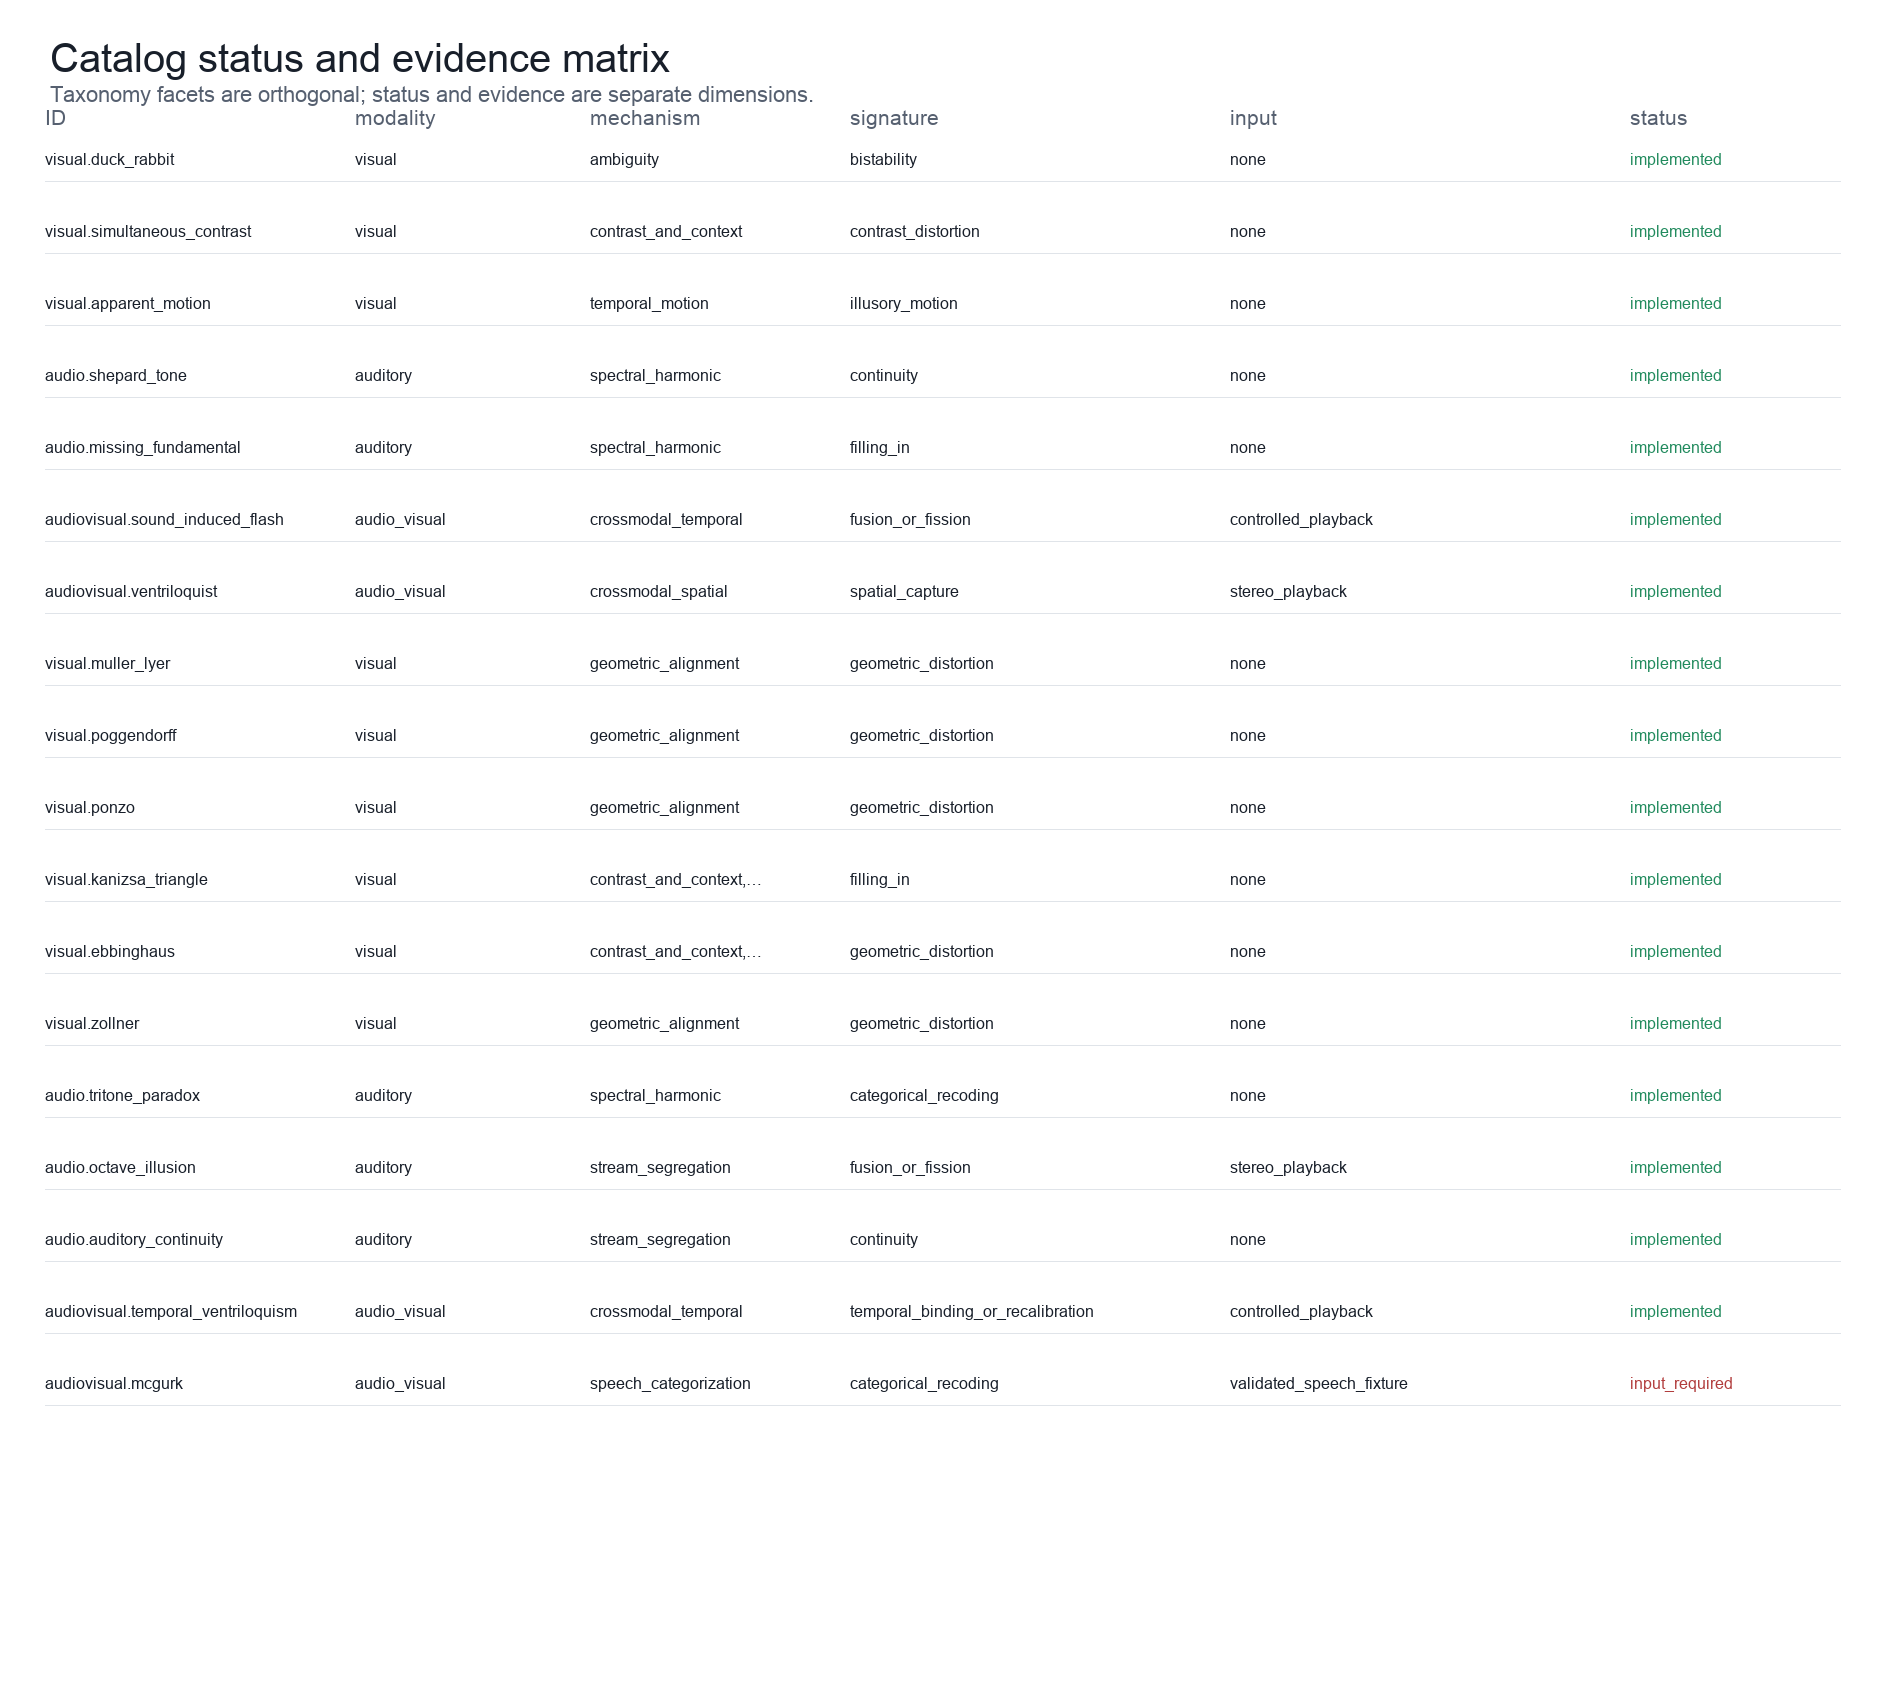
\includegraphics[keepaspectratio,alt={A matrix lists all catalog entries with modality, mechanism, signature, input requirement, and implementation status.}]{../figures/catalog_matrix.png}}
\caption{A matrix lists all catalog entries with modality, mechanism,
signature, input requirement, and implementation
status.}\label{fig:catalog_matrix}
\end{figure}

What this figure shows: A matrix lists all catalog entries with
modality, mechanism, signature, input requirement, and implementation
status. The live catalog matrix contains 18 entries and keeps modality,
mechanism, perceptual signature, input requirement, evidence status, and
implementation status as separate facets. Source data
output/data/catalog\_matrix.json preserve the exact taxonomy snapshot
and its source-reference namespace; status is not a proxy for perceptual
validation. Controls: live taxonomy registry; evidence matrix snapshot;
seed not applicable to the catalog diagram. Objective facts: 18 catalog
rows; categorical facets and statuses; no observer-level quantity is
applicable. Claim level: source\_supported. Source data:
output/data/catalog\_matrix.json (SHA-256 digest recorded in the figure
registry). Evidence lineage: gregory1997visual, hirst2020sound,
bruns2019ventriloquist. Limitations: Taxonomy facets are engineering
classifications and remain provisional where the literature supports
competing accounts. Boundary: Catalog coverage is bounded to this
registered package and does not enumerate all known illusions.

The complete catalog matrix fig.~\ref{fig:catalog_matrix} is tabulated
in the standalone Appendix A sec.~\ref{sec:appendix_catalog} and in
tbl.~\ref{tbl:catalog}. The corresponding machine-readable evidence
matrix records the source role, exact supported claim, engineering
departure, and limitation for every entry. Keeping the table in an
appendix gives the main results narrative room to explain the contract
without turning a mutable registry snapshot into a prose claim.

\subsection{Typed domains and delivery
profiles}\label{typed-domains-and-delivery-profiles}

\begin{longtable}[]{@{}
  >{\raggedright\arraybackslash}p{(\linewidth - 6\tabcolsep) * \real{0.2500}}
  >{\raggedright\arraybackslash}p{(\linewidth - 6\tabcolsep) * \real{0.2500}}
  >{\raggedright\arraybackslash}p{(\linewidth - 6\tabcolsep) * \real{0.2500}}
  >{\raggedright\arraybackslash}p{(\linewidth - 6\tabcolsep) * \real{0.2500}}@{}}
\caption{Typed parameter domains and
units.}\label{tbl:parameters}\tabularnewline
\toprule\noalign{}
\begin{minipage}[b]{\linewidth}\raggedright
Type
\end{minipage} & \begin{minipage}[b]{\linewidth}\raggedright
Unit
\end{minipage} & \begin{minipage}[b]{\linewidth}\raggedright
Validated domain
\end{minipage} & \begin{minipage}[b]{\linewidth}\raggedright
Role
\end{minipage} \\
\midrule\noalign{}
\endfirsthead
\toprule\noalign{}
\begin{minipage}[b]{\linewidth}\raggedright
Type
\end{minipage} & \begin{minipage}[b]{\linewidth}\raggedright
Unit
\end{minipage} & \begin{minipage}[b]{\linewidth}\raggedright
Validated domain
\end{minipage} & \begin{minipage}[b]{\linewidth}\raggedright
Role
\end{minipage} \\
\midrule\noalign{}
\endhead
\bottomrule\noalign{}
\endlastfoot
PixelDimension & pixels & 8--4096 & image/video width and height \\
GrayscaleLevels & levels & 2--256 & representable grayscale levels \\
QuantizationLevels & levels & 2--256 & output quantization buckets \\
FrequencyHz & Hz & \textgreater{} 0 and finite & oscillator and harmonic
frequencies \\
SampleRate & samples/s & 1,000--384,000 & audio sampling clock \\
FrameRate & frames/s & 1--240 & video presentation clock \\
SyncOffsetMs & ms & \texorpdfstring{\ensuremath{-}}{-}10,000--10,000 & audio relative to video \\
SpatialOffset & normalized & \texorpdfstring{\ensuremath{-}}{-}1--1 & declared crossmodal spatial
discrepancy \\
\end{longtable}

The parameter contracts are summarized in tbl.~\ref{tbl:parameters}.
They constrain physical construction and serialization; they are not
psychophysical scales.

\begin{longtable}[]{@{}
  >{\raggedright\arraybackslash}p{(\linewidth - 8\tabcolsep) * \real{0.2000}}
  >{\raggedright\arraybackslash}p{(\linewidth - 8\tabcolsep) * \real{0.2000}}
  >{\raggedright\arraybackslash}p{(\linewidth - 8\tabcolsep) * \real{0.2000}}
  >{\raggedright\arraybackslash}p{(\linewidth - 8\tabcolsep) * \real{0.2000}}
  >{\raggedright\arraybackslash}p{(\linewidth - 8\tabcolsep) * \real{0.2000}}@{}}
\caption{Encoding profiles and backend
capabilities.}\label{tbl:encodings}\tabularnewline
\toprule\noalign{}
\begin{minipage}[b]{\linewidth}\raggedright
Format
\end{minipage} & \begin{minipage}[b]{\linewidth}\raggedright
Backend
\end{minipage} & \begin{minipage}[b]{\linewidth}\raggedright
Artifact
\end{minipage} & \begin{minipage}[b]{\linewidth}\raggedright
Profile
\end{minipage} & \begin{minipage}[b]{\linewidth}\raggedright
Status
\end{minipage} \\
\midrule\noalign{}
\endfirsthead
\toprule\noalign{}
\begin{minipage}[b]{\linewidth}\raggedright
Format
\end{minipage} & \begin{minipage}[b]{\linewidth}\raggedright
Backend
\end{minipage} & \begin{minipage}[b]{\linewidth}\raggedright
Artifact
\end{minipage} & \begin{minipage}[b]{\linewidth}\raggedright
Profile
\end{minipage} & \begin{minipage}[b]{\linewidth}\raggedright
Status
\end{minipage} \\
\midrule\noalign{}
\endhead
\bottomrule\noalign{}
\endlastfoot
PNG & Pillow & image & lossless uint8 raster & available \\
WAV & python wave & audio & PCM 8/16/24/32-bit & available \\
GIF & Pillow & video & palette animation with declared duration &
available \\
NPZ & NumPy & canonical artifact & exact little-endian float32 archive &
available \\
MP4 & ffmpeg & video/audiovisual & H.264 or muxed MP4; decode inspected
& available \\
\end{longtable}

The delivery profiles are summarized in tbl.~\ref{tbl:encodings}.
Backend availability is environment-dependent and is recorded at
generation time.

The catalog distinguishes a physical construction from an observer
claim. For example, the sound-induced-flash generator establishes one
flash and one or two beep events on a shared clock; it does not
establish a reported flash count. Similarly, the temporal-ventriloquism
generator exposes a declared timing offset, while the literature reports
observer-dependent temporal judgments under specific tasks and timing
conditions \citep{vroomen2004temporal}.

\subsection{Pipeline and provenance}\label{pipeline-and-provenance}

\begin{figure}
\centering
\pandocbounded{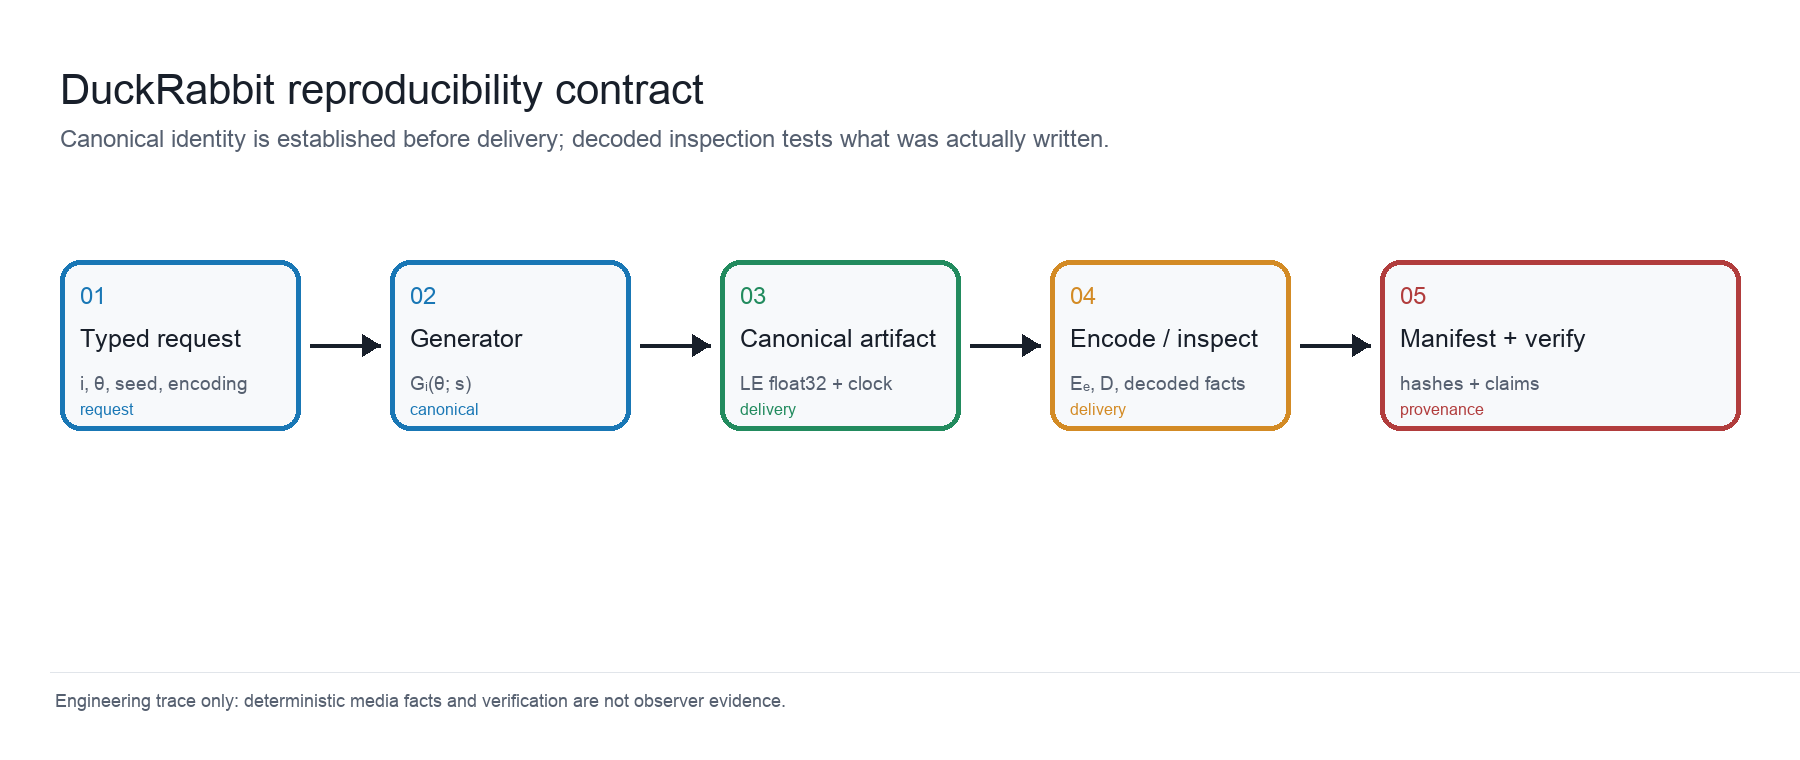
\includegraphics[keepaspectratio,alt={Five labeled stages connect a typed request to a deterministic canonical artifact, encoded media, decoded inspection, and a verification manifest.}]{../figures/architecture.png}}
\caption{Five labeled stages connect a typed request to a deterministic
canonical artifact, encoded media, decoded inspection, and a
verification manifest.}\label{fig:architecture}
\end{figure}

What this figure shows: Five labeled stages connect a typed request to a
deterministic canonical artifact, encoded media, decoded inspection, and
a verification manifest. This schematic separates a typed request from
the canonical artifact it generates, the optional delivery encoder,
decoded inspection, and the manifest-level verification decision. Arrows
indicate data and provenance dependencies rather than a causal model of
perception; the seed is 0 and the complete stage record is in source
data output/data/architecture.json. Controls: typed request q=(i,\texorpdfstring{\ensuremath{\theta}}{theta},s,e)
with seed s=0; default generator and delivery-independent
canonicalization. Objective facts: no unit-bearing objective quantity is
applicable to this architecture diagram; stage identities and provenance
fields are recorded in the sidecar. Claim level: canonical\_stimulus.
Source data: output/data/architecture.json (SHA-256 digest recorded in
the figure registry). Evidence lineage: formalism:eq:typed\_request,
formalism:eq:canonical\_generation, formalism:eq:encoding\_verification.
Limitations: The schematic abstracts implementation boundaries and does
not represent an observer study or a causal theory of perception.
Boundary: The pipeline verifies reproducible media facts, not what a
person experiences.

The generated architecture figure fig.~\ref{fig:architecture} shows the
separation between request, canonical artifact, delivery adapter,
decoded inspection, and manifest. The canonical digest is the identity
of the in-memory stimulus; an encoded hash is the identity of the
delivered file. The difference is intentional.

\subsection{Visual constructions and parameter
sweeps}\label{visual-constructions-and-parameter-sweeps}

\begin{figure}
\centering
\pandocbounded{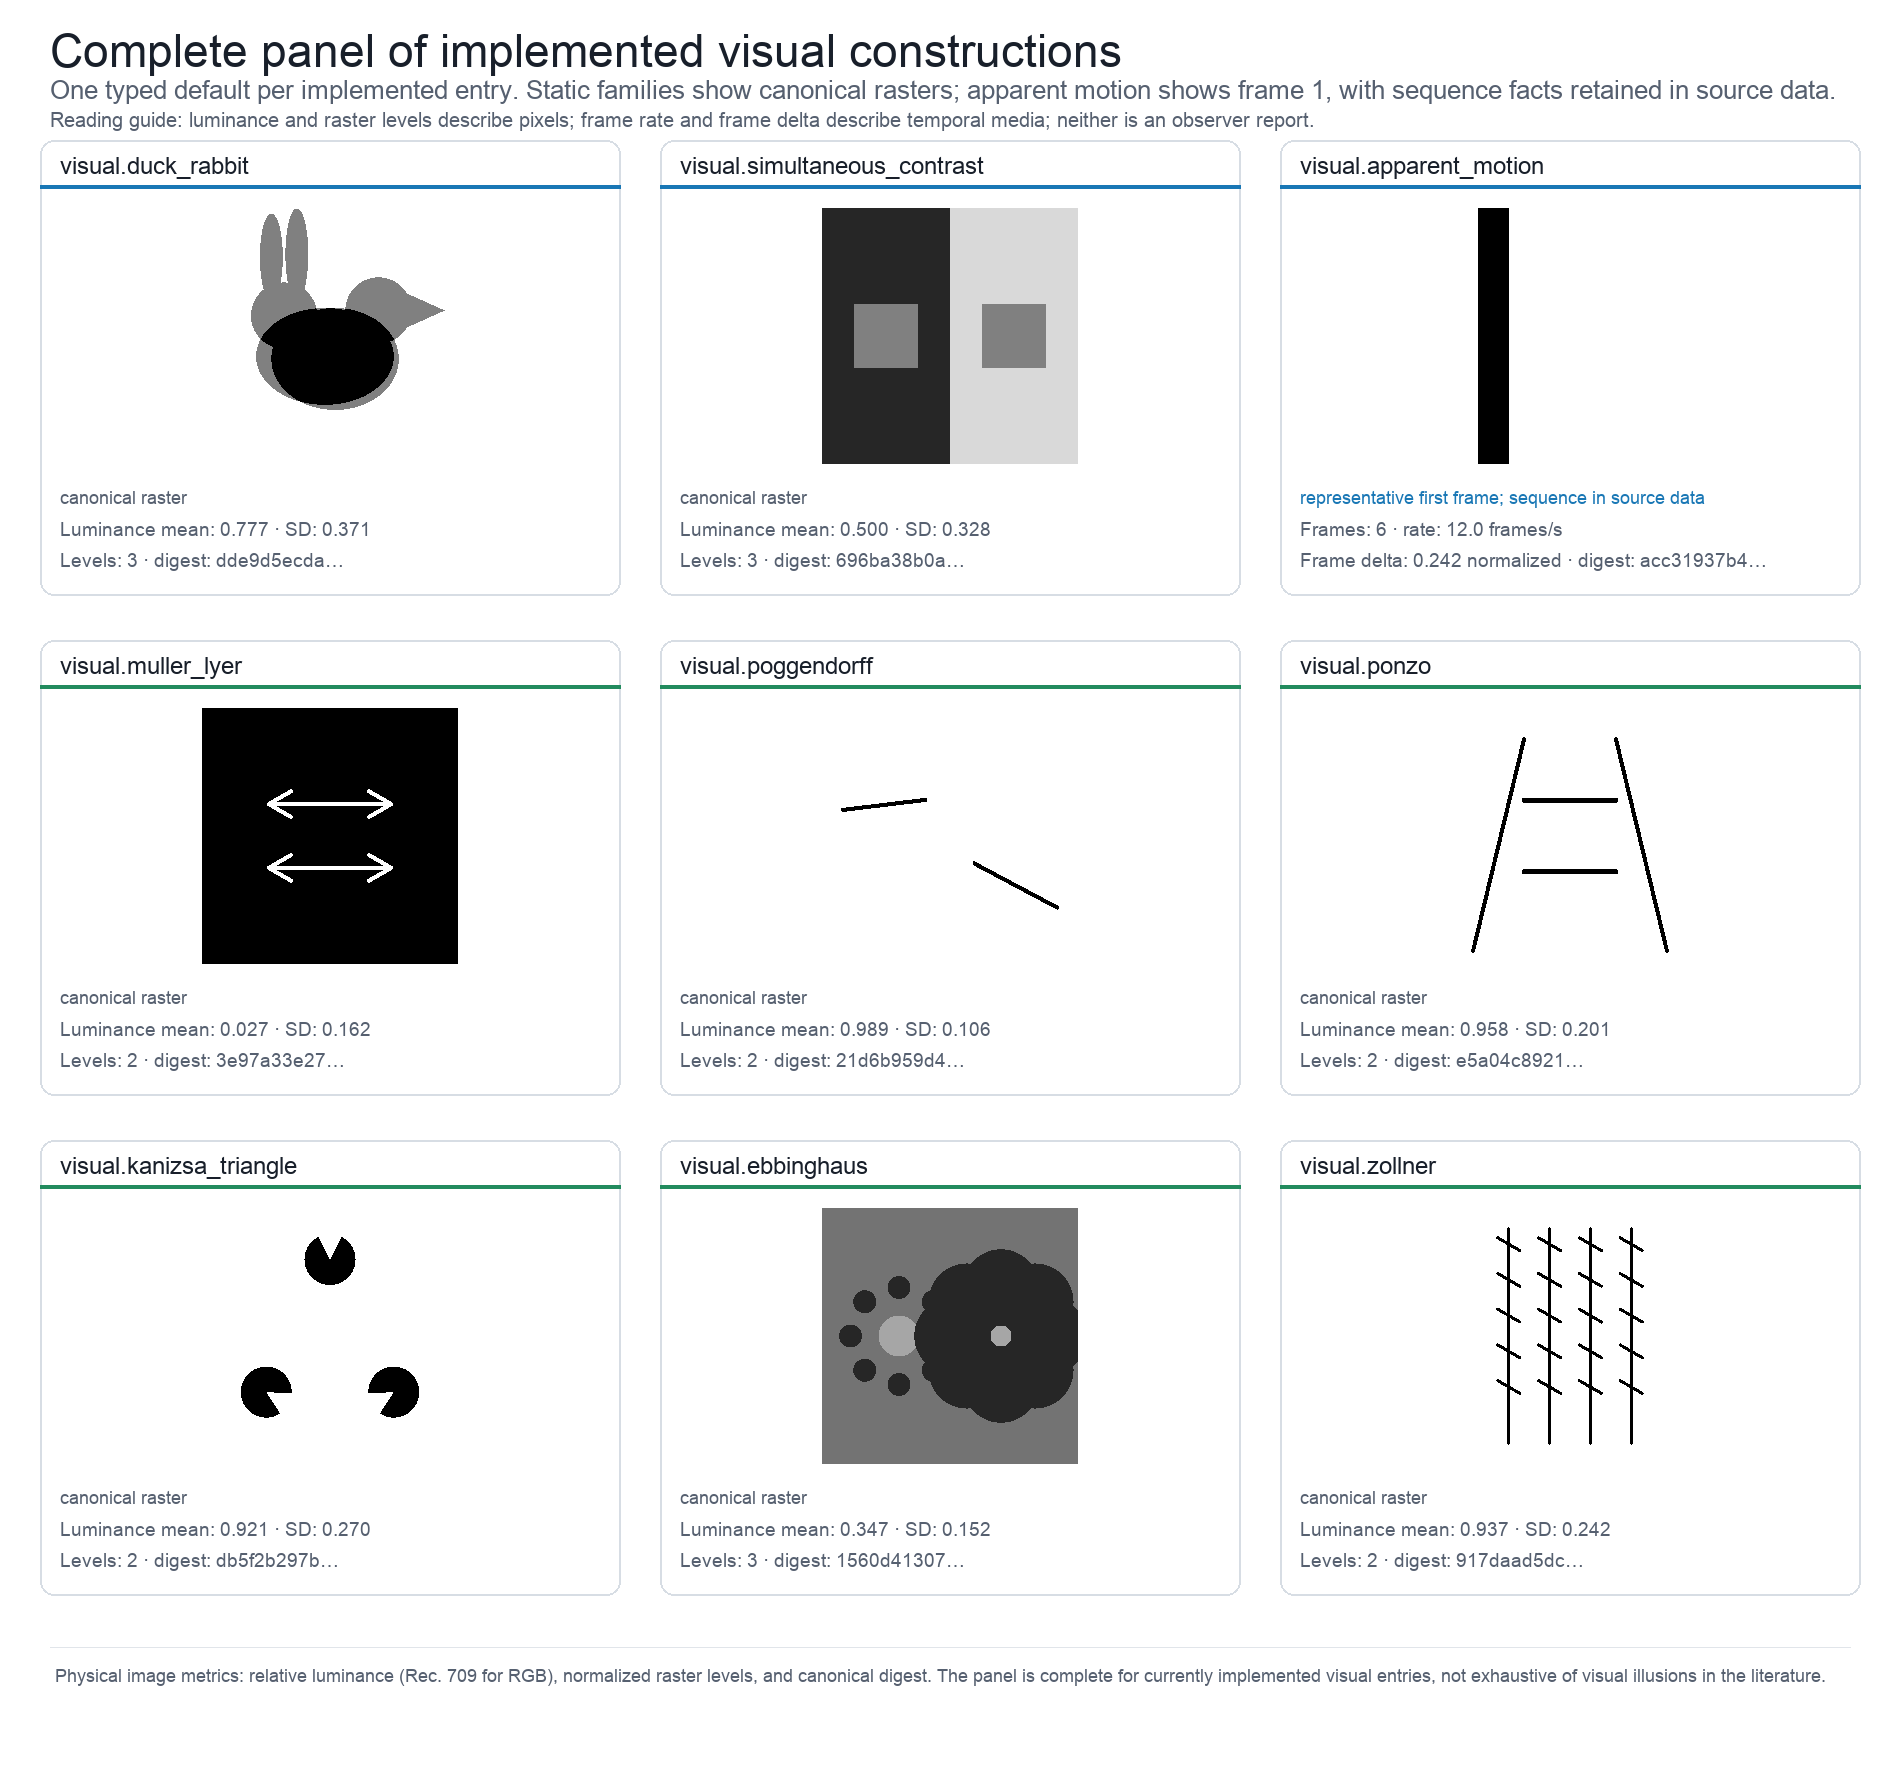
\includegraphics[keepaspectratio,alt={A 9-panel gallery shows every currently implemented visual catalog entry, with stable IDs and physical raster summaries: Duck-rabbit ambiguous figure, Simultaneous contrast stimulus, Apparent-motion frame sequence, Müller-Lyer geometric illusion, Poggendorff geometric illusion, Ponzo perspective illusion, Kanizsa illusory-contour triangle, Ebbinghaus context-size illusion, Zöllner orientation illusion.}]{../figures/visual_panel.png}}
\caption{A 9-panel gallery shows every currently implemented visual
catalog entry, with stable IDs and physical raster summaries:
Duck-rabbit ambiguous figure, Simultaneous contrast stimulus,
Apparent-motion frame sequence, Müller-Lyer geometric illusion,
Poggendorff geometric illusion, Ponzo perspective illusion, Kanizsa
illusory-contour triangle, Ebbinghaus context-size illusion, Zöllner
orientation illusion.}\label{fig:visual_panel}
\end{figure}

What this figure shows: A 9-panel gallery shows every currently
implemented visual catalog entry, with stable IDs and physical raster
summaries: Duck-rabbit ambiguous figure, Simultaneous contrast stimulus,
Apparent-motion frame sequence, Müller-Lyer geometric illusion,
Poggendorff geometric illusion, Ponzo perspective illusion, Kanizsa
illusory-contour triangle, Ebbinghaus context-size illusion, Zöllner
orientation illusion. This complete gallery presents one deterministic
representative from each of the 9 currently implemented visual catalog
entries: Duck-rabbit ambiguous figure, Simultaneous contrast stimulus,
Apparent-motion frame sequence, Müller-Lyer geometric illusion,
Poggendorff geometric illusion, Ponzo perspective illusion, Kanizsa
illusory-contour triangle, Ebbinghaus context-size illusion, Zöllner
orientation illusion. The panel therefore covers the package's available
visual families---ambiguous figure, contrast, apparent motion, geometric
context, illusory contour, contextual size, and orientation-related
constructions---using typed defaults at seed 0. For the temporally
expressed apparent-motion entry, the displayed tile is its first frame
and the source data preserve the full sequence. The source data sidecar
output/data/visual\_panel.json records the stable ID, generator
parameters, canonical SHA-256 digest, Rec. 709 or grayscale luminance
statistics, raster-level counts, and parameter boundary for every tile.
Controls: one default typed parameter object per implemented visual
entry; seed s=0; dimensions, luminance bounds, grayscale, and
quantization controls remain in each generator schema; temporal entries
display their first frame but retain sequence metrics. Objective facts:
per tile: mean and standard-deviation relative luminance, unique raster
levels, and canonical SHA-256 digest; temporal entries additionally
retain frame count, frame rate, and frame deltas; definitions and units
are in the source data JSON. Claim level: canonical\_stimulus. Source
data: output/data/visual\_panel.json (SHA-256 digest recorded in the
figure registry). Evidence lineage: gregory1997visual,
brugger1999duckrabbit, howe2005muller, morgan1999poggendorff,
fisher1967ponzo, yildiz2022ponzo, kanizsa1976contours,
mruczek2015ebbinghaus, earle1995zollner, wertheimer1912motion,
sekuler1996wertheimer. Limitations: The gallery is complete for
implemented visual entries in this package, not a complete survey of
visual illusions; literature families, historical displays, and
DuckRabbit rasters are not pixel-identical by default. Viewing scale,
display calibration, viewing distance, and observer conditions can
change the relevance of a construction; the gallery does not measure an
observer's perceptual report. Boundary: The figure establishes coverage
of the package's implemented visual constructions and their
deterministic raster facts. It does not establish that any viewer will
perceive the named signature, nor that the set is exhaustive of the
visual-illusion literature.

The visual panel fig.~\ref{fig:visual_panel} is deliberately a coverage
figure: it contains one deterministic representative for every currently
implemented visual entry, including apparent motion and Zöllner in
addition to the static ambiguous-figure, contrast, geometric-context,
illusory-contour, and contextual- size families. Equalities, masks, line
geometry, luminance bounds, and temporal positions are properties of the
typed rasters or sequences. They are not observer scores, and the
gallery is not an exhaustive ontology of visual illusions.

\begin{figure}
\centering
\pandocbounded{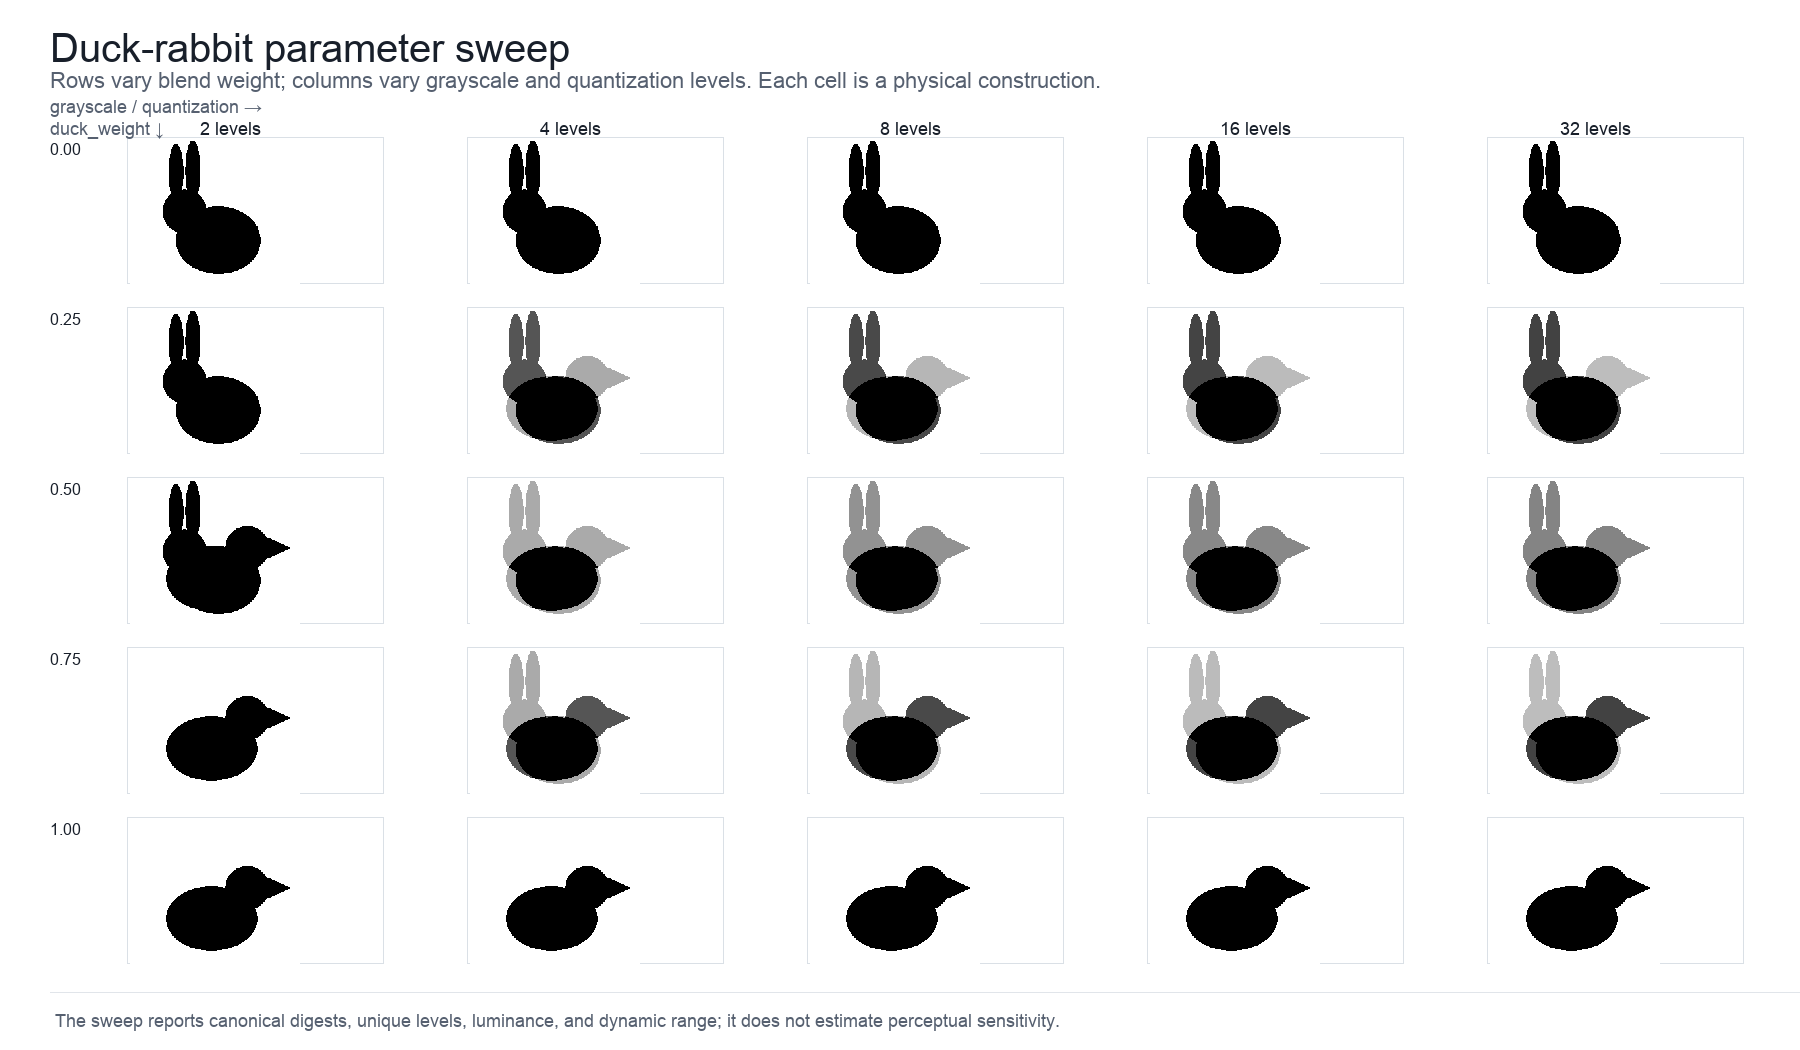
\includegraphics[keepaspectratio,alt={A labeled grid crosses five duck--rabbit blend weights with five grayscale and quantization settings, with physical metrics recorded for each cell.}]{../figures/visual_sweep.png}}
\caption{A labeled grid crosses five duck--rabbit blend weights with
five grayscale and quantization settings, with physical metrics recorded
for each cell.}\label{fig:visual_sweep}
\end{figure}

What this figure shows: A labeled grid crosses five duck--rabbit blend
weights with five grayscale and quantization settings, with physical
metrics recorded for each cell. This 5\texorpdfstring{\ensuremath{\times}}{x}5 sweep varies duck--rabbit blend
weight across rows and jointly varies grayscale and quantization levels
across columns. Each cell is regenerated from an immutable typed
parameter object at seed 0; source data output/data/visual\_sweep.json
records canonical digests, unique-level counts, normalized luminance,
and effective dynamic range for every condition. Controls: duck\_weight
\texorpdfstring{\ensuremath{\in}}{in} \{0,.25,.5,.75,1\}; grayscale=quantization \texorpdfstring{\ensuremath{\in}}{in} \{2,4,8,16,32\}; seed
s=0. Objective facts: 25 canonical rasters; unique levels, normalized
mean luminance, and effective dynamic range per cell. Claim level:
physical\_metric. Source data: output/data/visual\_sweep.json (SHA-256
digest recorded in the figure registry). Evidence lineage:
brugger1999duckrabbit, gregory1997visual. Limitations: The grid is a
sensitivity of the construction parameters, not a psychophysical
sensitivity curve or a validated observer effect. Boundary: The chosen
grid is an engineering sampling of the parameter domain and does not
imply an optimal or perceptually uniform spacing.

The sweep fig.~\ref{fig:visual_sweep} varies duck-weight from 0 to 1 and
jointly varies representable grayscale and quantization levels. The
source data preserve canonical digests and unique-value counts; no
perceptual score is assigned to a sweep cell.

\subsection{Temporal and auditory
constructions}\label{temporal-and-auditory-constructions}

\begin{figure}
\centering
\pandocbounded{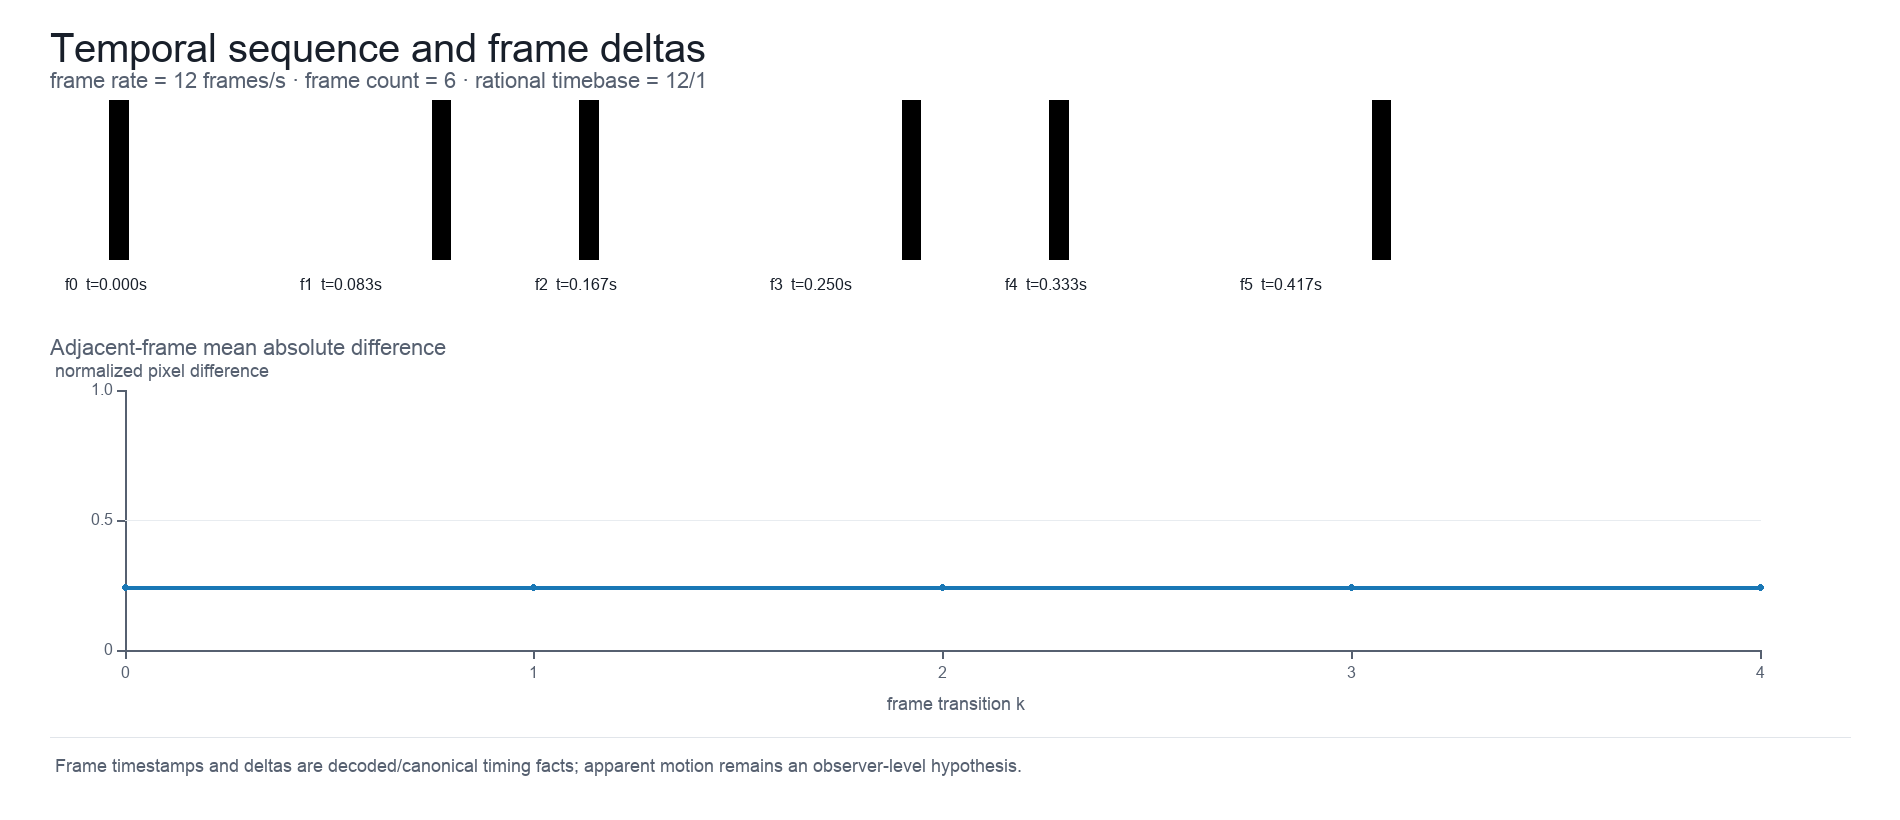
\includegraphics[keepaspectratio,alt={Six ordered frames are labeled with timestamps and paired with a line plot of adjacent-frame normalized pixel differences.}]{../figures/temporal_sequence.png}}
\caption{Six ordered frames are labeled with timestamps and paired with
a line plot of adjacent-frame normalized pixel
differences.}\label{fig:temporal_sequence}
\end{figure}

What this figure shows: Six ordered frames are labeled with timestamps
and paired with a line plot of adjacent-frame normalized pixel
differences. The frame strip exposes the order and timestamps of the
apparent-motion construction, while the lower trace reports
adjacent-frame mean absolute pixel differences. Source data
output/data/temporal\_sequence.json preserve frame count, frame rate,
reduced rational timebase, timestamps in seconds, and the nonzero
transition series; seed 0 identifies the generated sequence. Controls:
visual.apparent\_motion default typed parameters; frame rate and frame
count from the canonical sequence; seed s=0. Objective facts: timestamps
in seconds, frame rate in frames/s, frame count, rational timebase, and
adjacent-frame normalized pixel difference. Claim level:
physical\_metric. Source data: output/data/temporal\_sequence.json
(SHA-256 digest recorded in the figure registry). Evidence lineage:
wertheimer1912motion, sekuler1996wertheimer. Limitations: Frame
succession and frame deltas are physical file properties; playback
timing, display persistence, and motion reports require a controlled
observer task. Boundary: The figure documents temporal structure rather
than the presence, direction, or strength of perceived motion.

The temporal figure fig.~\ref{fig:temporal_sequence} reports frame
succession, rational frame rate, and frame-to-frame mean absolute
differences. These facts establish temporal structure in the file, not
the presence or strength of perceived motion.

\begin{figure}
\centering
\pandocbounded{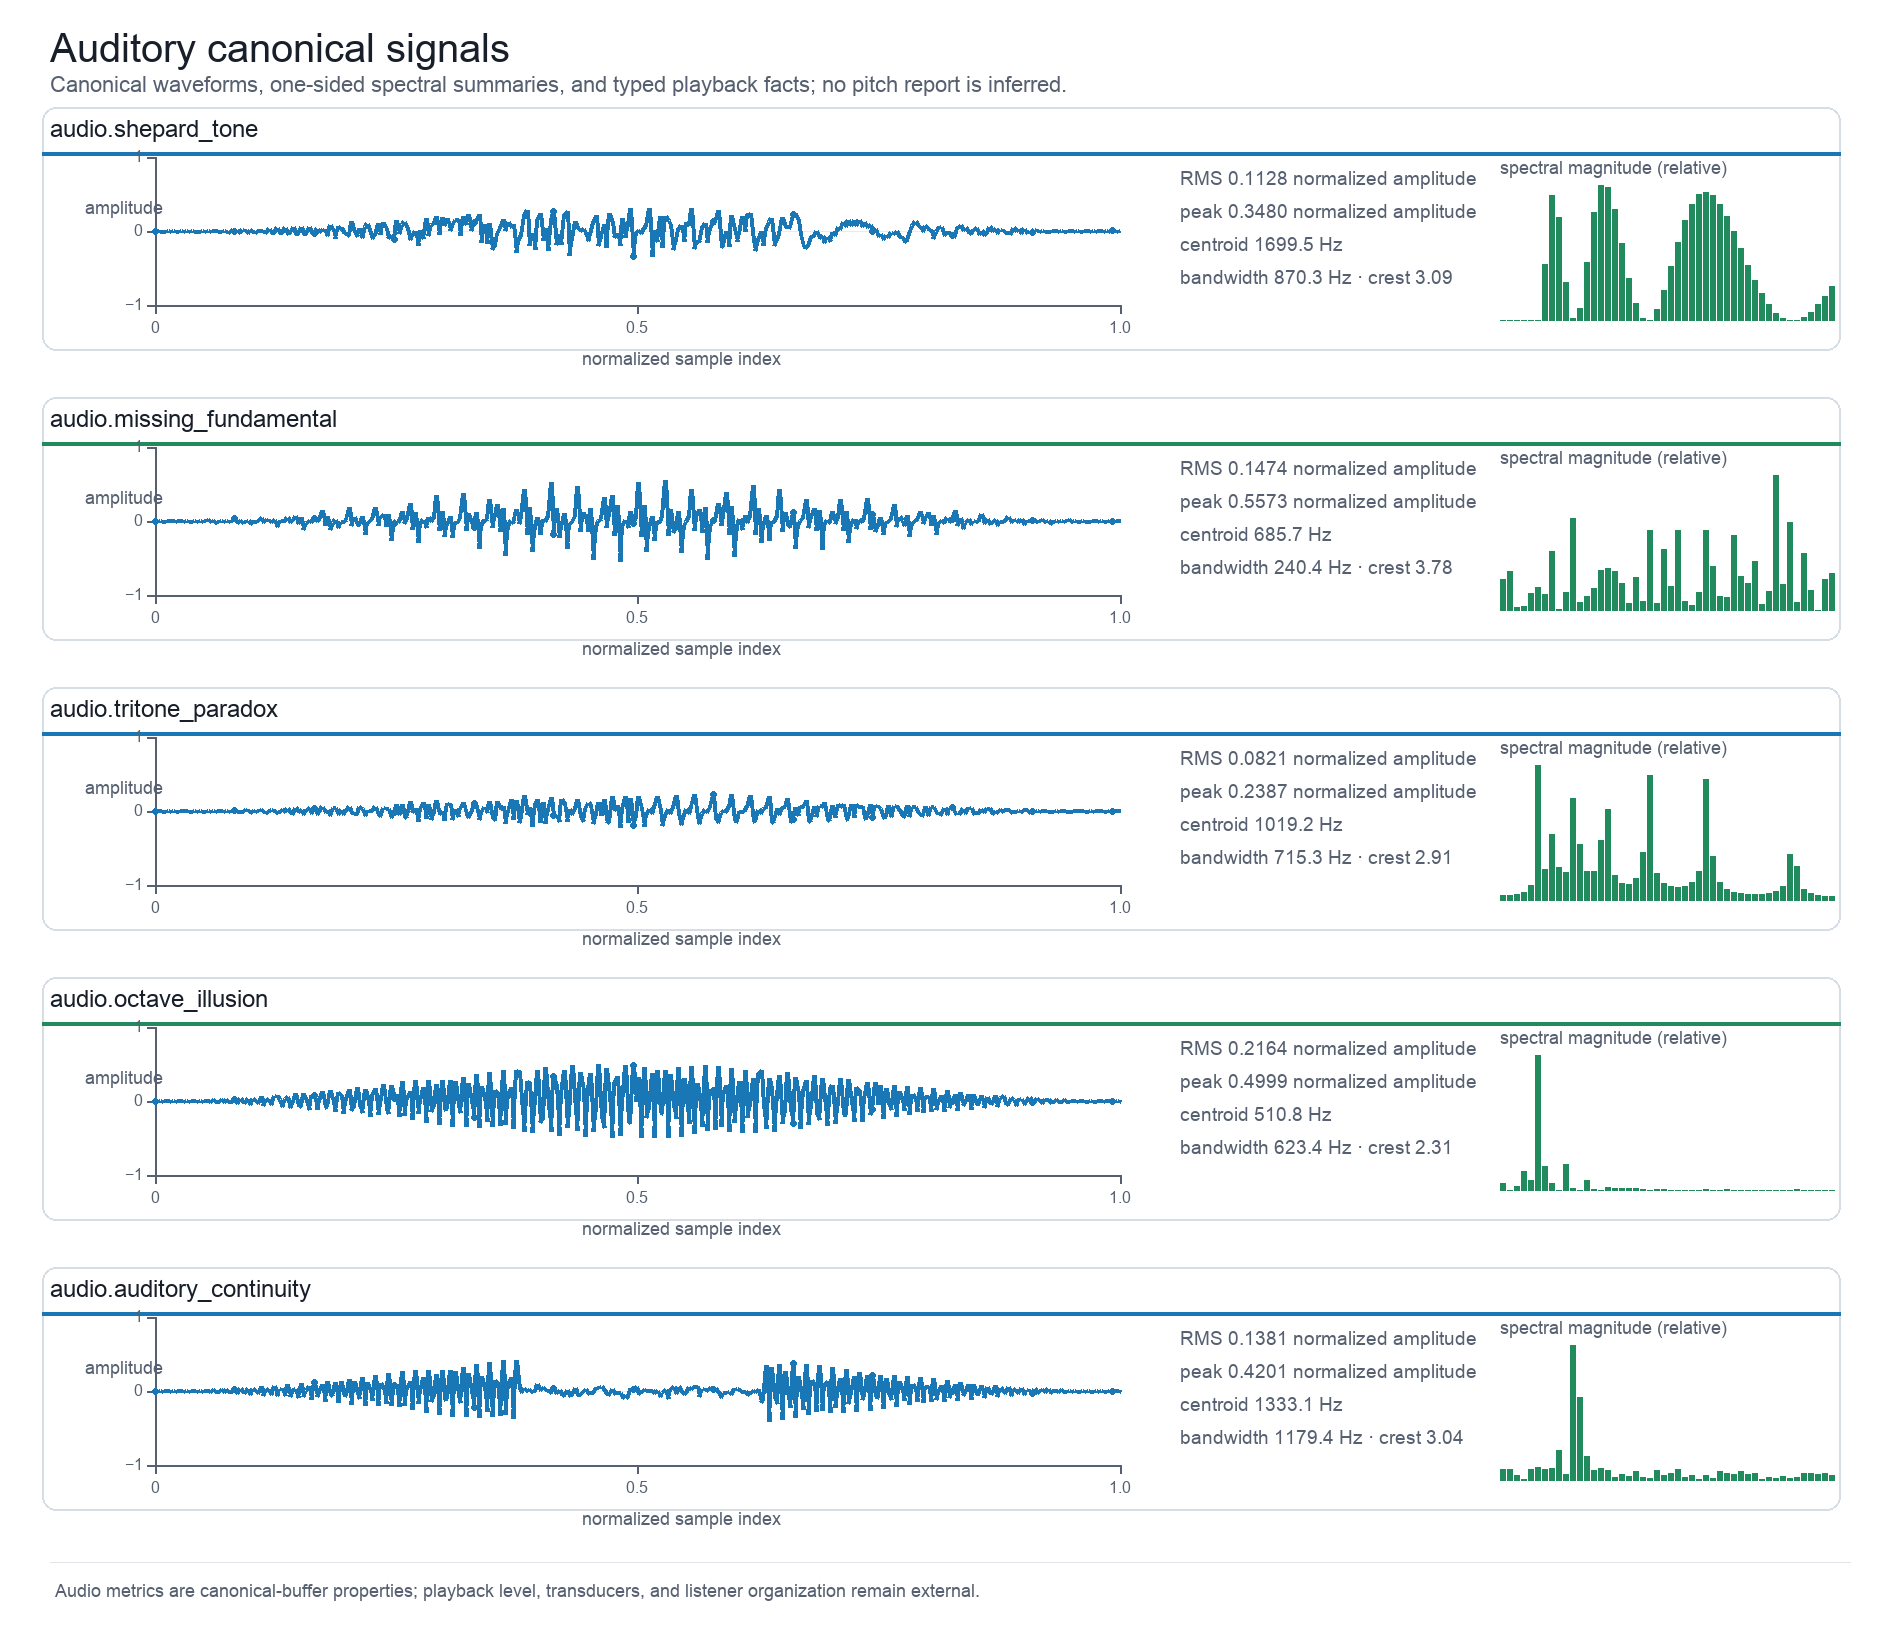
\includegraphics[keepaspectratio,alt={Five labeled rows show canonical audio waveforms, relative one-sided spectral bars, RMS and peak in normalized amplitude, and spectral summaries in hertz.}]{../figures/audio_signals.png}}
\caption{Five labeled rows show canonical audio waveforms, relative
one-sided spectral bars, RMS and peak in normalized amplitude, and
spectral summaries in hertz.}\label{fig:audio_signals}
\end{figure}

What this figure shows: Five labeled rows show canonical audio
waveforms, relative one-sided spectral bars, RMS and peak in normalized
amplitude, and spectral summaries in hertz. Five implemented auditory
constructions---Shepard tone, missing fundamental, tritone paradox,
octave illusion, and auditory continuity---are shown as canonical
waveforms with compact one-sided FFT summaries. Source data
output/data/audio\_signals.json records sample rate, channel layout,
RMS, peak, spectral centroid, bandwidth, crest factor, canonical digest,
and the declared display-bin convention; no pitch or stream report is
inferred. Controls: default typed audio parameters; per-generator
channel layout and sample rate; seed s=0; one-sided FFT display with 48
sampled bins. Objective facts: RMS and peak in normalized amplitude;
spectral centroid and bandwidth in Hz; sample rate in samples/s; channel
layout and canonical SHA-256 digest. Claim level: physical\_metric.
Source data: output/data/audio\_signals.json (SHA-256 digest recorded in
the figure registry). Evidence lineage: shepard1984scale,
zatorre2005missing, deutsch1986tritone, repp1997tritone,
deutsch1974octave, warren1970continuity, riecke2011continuity.
Limitations: Playback level, transducer response, dichotic separation,
masker design, and listener judgments are external to the canonical
buffer. Boundary: The figure compares generated signal properties and
literature-linked families; it does not establish pitch, continuity, or
stream organization for a listener.

The auditory figure fig.~\ref{fig:audio_signals} shows canonical
waveforms and spectral summaries for Shepard, missing-fundamental,
tritone, octave, and continuity constructions. RMS, peak, spectral
centroid, bandwidth, and channel layout are calculated from the
canonical buffer with explicit units and windowing rules. Pitch
direction, pitch height, continuity, and stream organization remain
observer-level outcomes that depend on playback and task conditions.

\subsection{Audiovisual timing and
encoding}\label{audiovisual-timing-and-encoding}

\begin{figure}
\centering
\pandocbounded{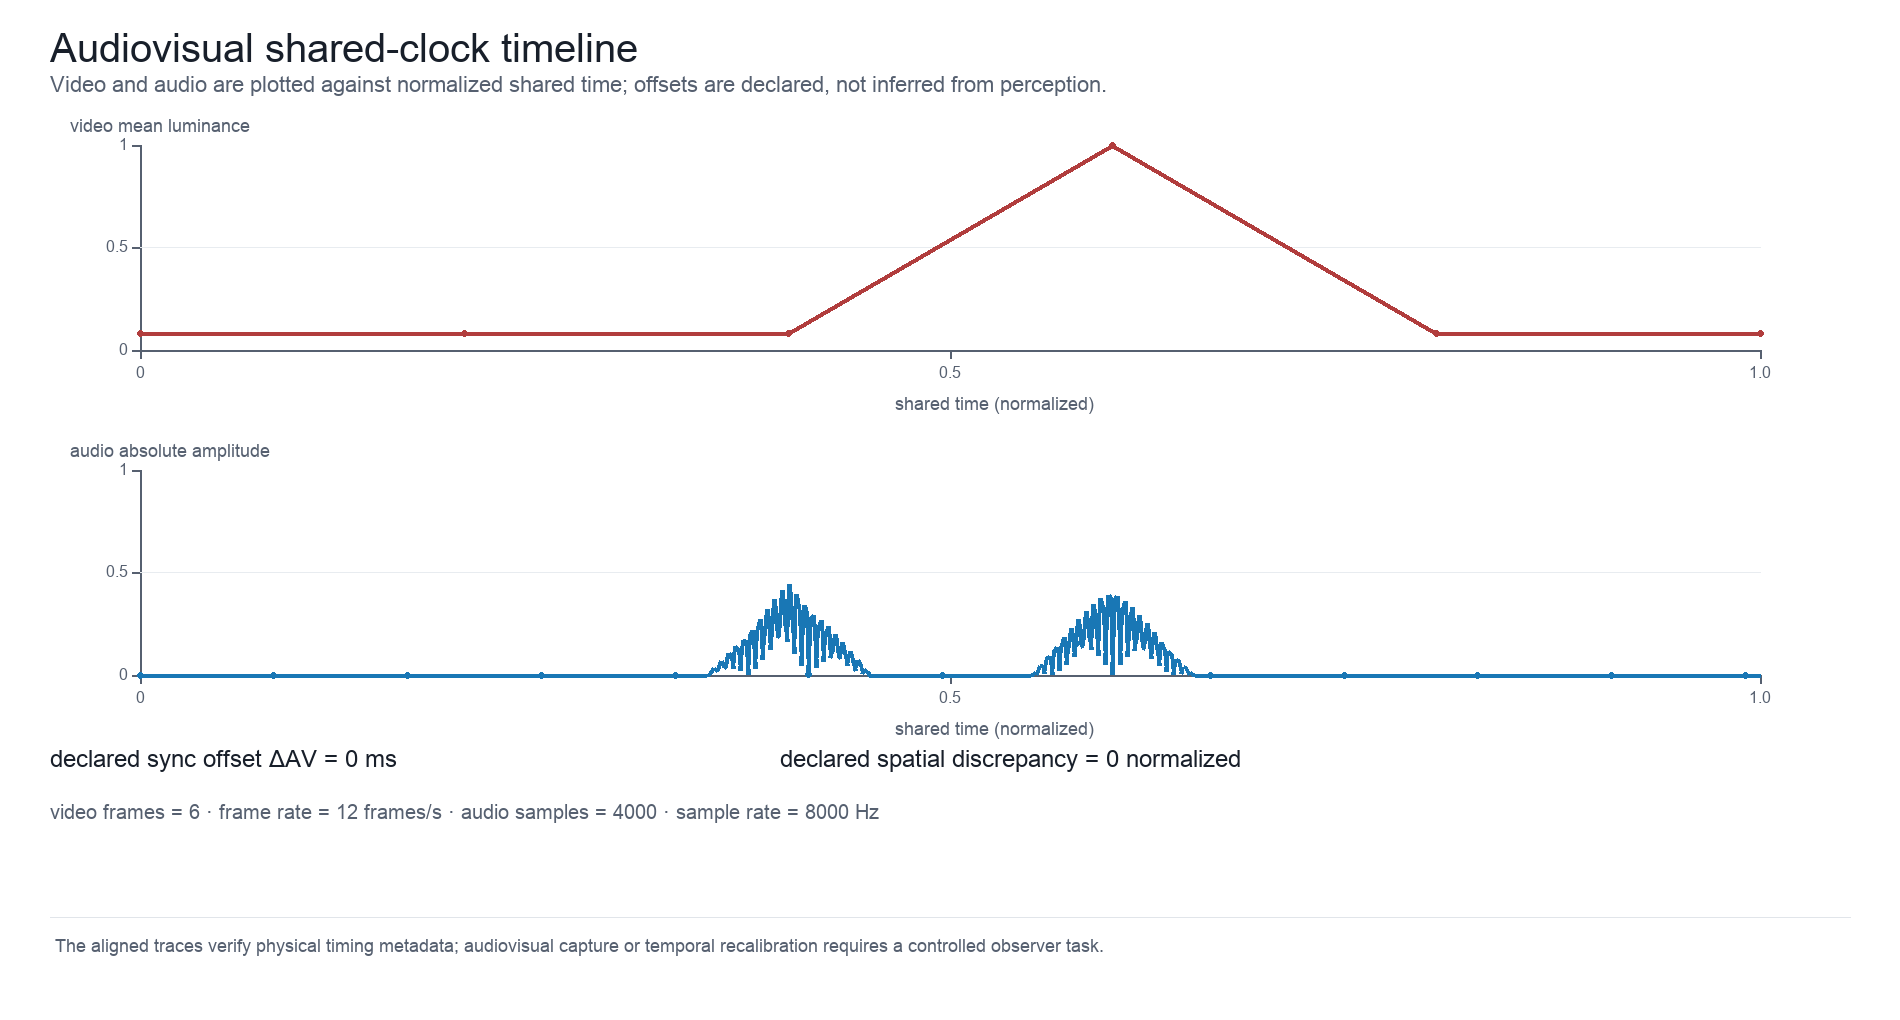
\includegraphics[keepaspectratio,alt={Two labeled traces share a normalized time axis: video mean luminance and audio absolute amplitude, with signed synchronization and spatial offsets printed below.}]{../figures/audiovisual_timeline.png}}
\caption{Two labeled traces share a normalized time axis: video mean
luminance and audio absolute amplitude, with signed synchronization and
spatial offsets printed below.}\label{fig:audiovisual_timeline}
\end{figure}

What this figure shows: Two labeled traces share a normalized time axis:
video mean luminance and audio absolute amplitude, with signed
synchronization and spatial offsets printed below. Video mean luminance
and rectified audio amplitude are placed on a common normalized time
axis for the sound-induced-flash construction. Source data
output/data/audiovisual\_timeline.json records the video frame clock,
audio sampling clock, event traces, signed audio-minus-video
synchronization offset in milliseconds, and normalized spatial
discrepancy; alignment is declared by the generator, not estimated from
perception. Controls: audiovisual.sound\_induced\_flash default shared
timeline; declared sync offset \texorpdfstring{\ensuremath{\Delta}}{Delta}AV and spatial offset; seed s=0.
Objective facts: video luminance and audio envelope on normalized shared
time; \texorpdfstring{\ensuremath{\Delta}}{Delta}AV in ms; spatial discrepancy in normalized units; frame and
sample clocks in the sidecar. Claim level: physical\_metric. Source
data: output/data/audiovisual\_timeline.json (SHA-256 digest recorded in
the figure registry). Evidence lineage: shams2000sifi, hirst2020sound,
vroomen2004temporal, hartcherobrien2011temporal. Limitations: Display
refresh, audio hardware, event latency, and observer temporal binding
are not measured by this figure. Boundary: A shared-clock construction
is not evidence that observers bind the events at the declared or any
other perceptual time.

The audiovisual timeline fig.~\ref{fig:audiovisual_timeline} displays
video luminance and audio amplitude against the shared clock, alongside
declared synchronization and spatial offsets. Ventriloquist stimuli
require stereo playback and spatially resolved display; temporal binding
requires controlled timing and an observer task
\citep{bruns2019ventriloquist, vroomen2004temporal}.

\begin{figure}
\centering
\pandocbounded{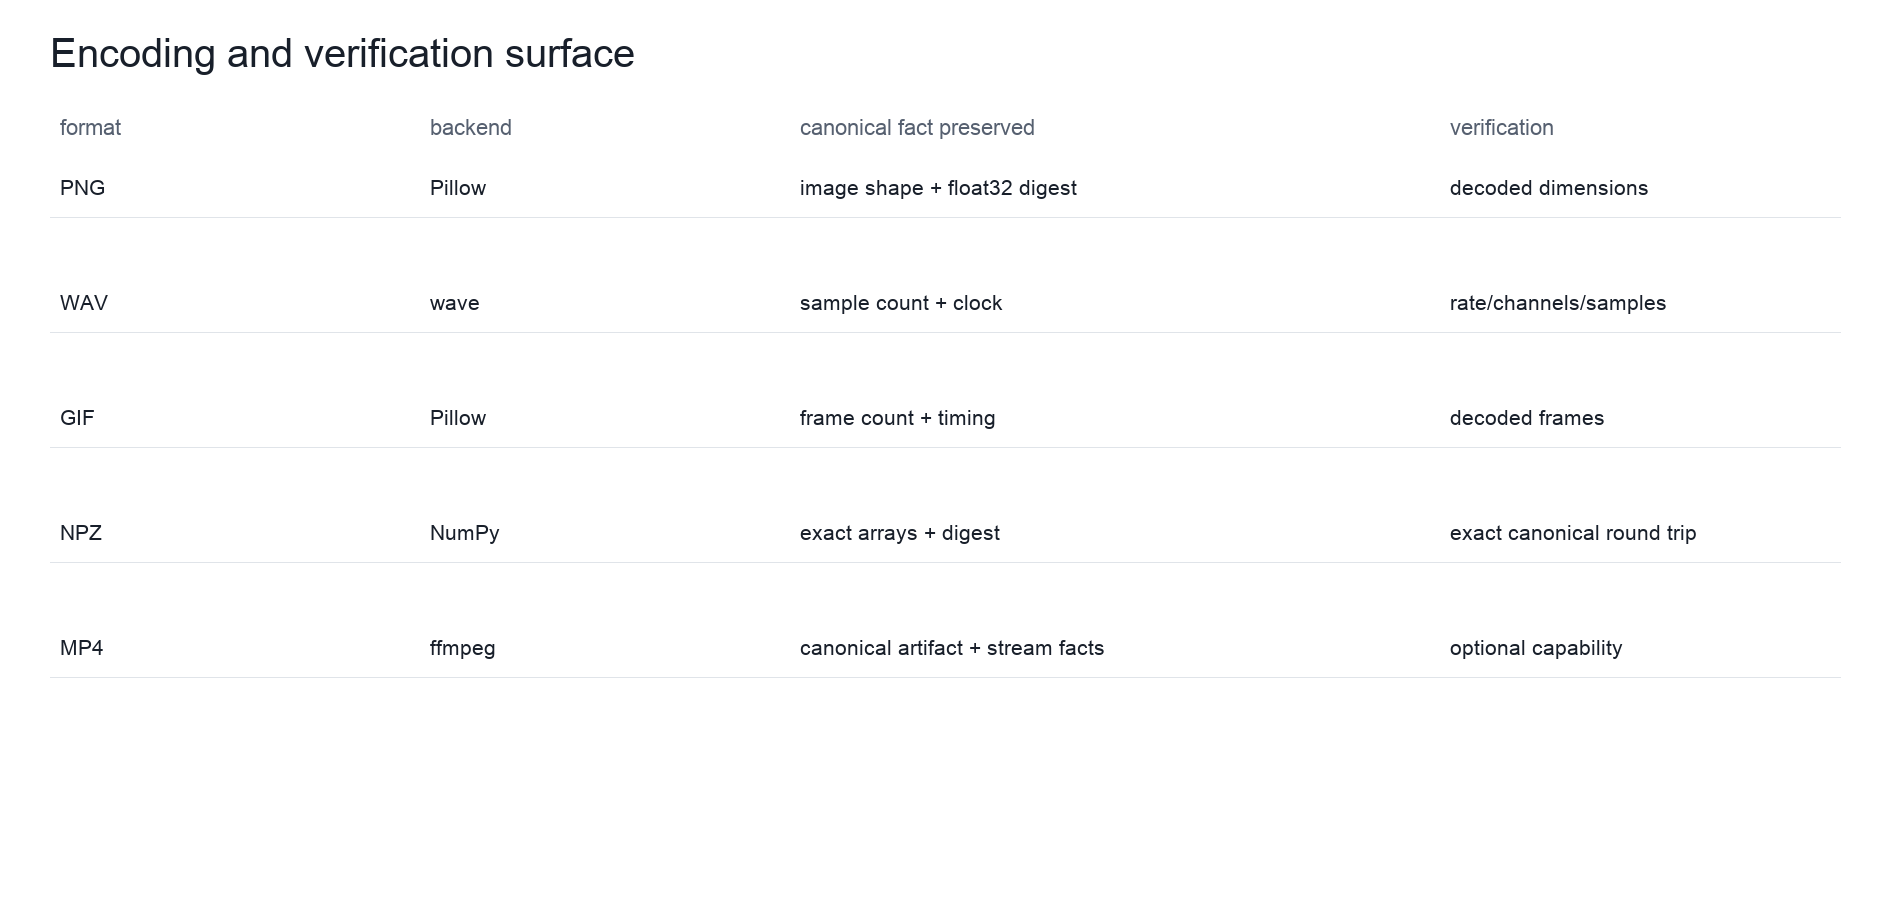
\includegraphics[keepaspectratio,alt={A five-row comparison lists format, backend, preserved canonical facts, and the corresponding decoded verification checks.}]{../figures/encoding_verification.png}}
\caption{A five-row comparison lists format, backend, preserved
canonical facts, and the corresponding decoded verification
checks.}\label{fig:encoding_verification}
\end{figure}

What this figure shows: A five-row comparison lists format, backend,
preserved canonical facts, and the corresponding decoded verification
checks. The comparison separates the canonical artifact from delivery
containers: PNG, WAV, GIF, NPZ, and optional MP4/muxed MP4. Source data
output/data/encoding\_verification.json records backend identity,
preserved canonical facts, decoded inspection targets, and capability
status as observed in the generation environment; the table therefore
describes an adapter contract rather than a claim about codec quality.
Controls: typed encoding profile selected per artifact; overwrite and
backend capability checks; seed inherited from the stimulus request.
Objective facts: format availability and verification scope are
environment observations; NPZ is exact while other formats are decoded
and tolerance-checked. Claim level: encoded\_media. Source data:
output/data/encoding\_verification.json (SHA-256 digest recorded in the
figure registry). Evidence lineage: engineering:typed\_media\_adapters.
Limitations: Backend availability, codec versions, container metadata,
and lossy tolerances are environment-dependent; playback software can
expose additional behavior. Boundary: A successful encode or decode does
not validate an observer effect or guarantee cross-device perceptual
equivalence.

The encoding matrix fig.~\ref{fig:encoding_verification} makes backend
capability and verification scope visible. NPZ is the exact canonical
archive; PNG, WAV, GIF, and MP4 are delivery containers whose decoded
facts are checked against the manifest.

\subsection{Objective metric
results}\label{sec:objective_metric_results}

\begin{longtable}[]{@{}
  >{\raggedright\arraybackslash}p{(\linewidth - 8\tabcolsep) * \real{0.2000}}
  >{\raggedright\arraybackslash}p{(\linewidth - 8\tabcolsep) * \real{0.2000}}
  >{\raggedright\arraybackslash}p{(\linewidth - 8\tabcolsep) * \real{0.2000}}
  >{\raggedright\arraybackslash}p{(\linewidth - 8\tabcolsep) * \real{0.2000}}
  >{\raggedright\arraybackslash}p{(\linewidth - 8\tabcolsep) * \real{0.2000}}@{}}
\caption{Objective metric definitions and epistemic
boundary.}\label{tbl:metrics}\tabularnewline
\toprule\noalign{}
\begin{minipage}[b]{\linewidth}\raggedright
Metric
\end{minipage} & \begin{minipage}[b]{\linewidth}\raggedright
Unit
\end{minipage} & \begin{minipage}[b]{\linewidth}\raggedright
Definition
\end{minipage} & \begin{minipage}[b]{\linewidth}\raggedright
Tolerance
\end{minipage} & \begin{minipage}[b]{\linewidth}\raggedright
Claim level
\end{minipage} \\
\midrule\noalign{}
\endfirsthead
\toprule\noalign{}
\begin{minipage}[b]{\linewidth}\raggedright
Metric
\end{minipage} & \begin{minipage}[b]{\linewidth}\raggedright
Unit
\end{minipage} & \begin{minipage}[b]{\linewidth}\raggedright
Definition
\end{minipage} & \begin{minipage}[b]{\linewidth}\raggedright
Tolerance
\end{minipage} & \begin{minipage}[b]{\linewidth}\raggedright
Claim level
\end{minipage} \\
\midrule\noalign{}
\endhead
\bottomrule\noalign{}
\endlastfoot
mean\_luminance & normalized\_luminance & mean Rec. 709 relative
luminance (grayscale is identity) & exact canonical &
physical\_metric \\
unique\_values & levels & count of distinct canonical image values &
exact integer & physical\_metric \\
rms & normalized\_amplitude & root-mean-square audio amplitude & finite
scalar & physical\_metric \\
peak & normalized\_amplitude & maximum absolute audio amplitude & finite
scalar & physical\_metric \\
spectral\_centroid\_hz & Hz & energy-weighted one-sided spectral
centroid & finite scalar & physical\_metric \\
spectral\_bandwidth\_hz & Hz & spectral standard deviation around the
one-sided centroid & finite scalar & physical\_metric \\
crest\_factor & ratio & audio peak divided by RMS with zero-RMS guard &
finite scalar & physical\_metric \\
mean\_temporal\_delta & normalized\_pixel\_difference & mean
adjacent-frame absolute difference & finite scalar & physical\_metric \\
sync\_offset & ms & declared audio-minus-video offset & typed value &
physical\_metric \\
\end{longtable}

The metric definitions in tbl.~\ref{tbl:metrics} are computed from
canonical or decoded artifacts and do not encode observer
interpretations.

The default duck-rabbit artifact contains 3 unique raster levels and has
mean normalized luminance 0.7770. These values are live generated facts,
not perceptual effect sizes.

\subsection{Observer estimands and verification
controls}\label{observer-estimands-and-verification-controls}

\begin{longtable}[]{@{}
  >{\raggedright\arraybackslash}p{(\linewidth - 6\tabcolsep) * \real{0.2500}}
  >{\raggedright\arraybackslash}p{(\linewidth - 6\tabcolsep) * \real{0.2500}}
  >{\raggedright\arraybackslash}p{(\linewidth - 6\tabcolsep) * \real{0.2500}}
  >{\raggedright\arraybackslash}p{(\linewidth - 6\tabcolsep) * \real{0.2500}}@{}}
\caption{Data-free observer outcomes and preregistered
estimands.}\label{tbl:observer_estimands}\tabularnewline
\toprule\noalign{}
\begin{minipage}[b]{\linewidth}\raggedright
Estimand
\end{minipage} & \begin{minipage}[b]{\linewidth}\raggedright
Response and model
\end{minipage} & \begin{minipage}[b]{\linewidth}\raggedright
Reference and contrast
\end{minipage} & \begin{minipage}[b]{\linewidth}\raggedright
Uncertainty
\end{minipage} \\
\midrule\noalign{}
\endfirsthead
\toprule\noalign{}
\begin{minipage}[b]{\linewidth}\raggedright
Estimand
\end{minipage} & \begin{minipage}[b]{\linewidth}\raggedright
Response and model
\end{minipage} & \begin{minipage}[b]{\linewidth}\raggedright
Reference and contrast
\end{minipage} & \begin{minipage}[b]{\linewidth}\raggedright
Uncertainty
\end{minipage} \\
\midrule\noalign{}
\endhead
\bottomrule\noalign{}
\endlastfoot
sifi flash count contrast & event count; poisson or ordinal & sifi one
beep; two-beep minus one-beep event-count response & 95\% confidence
interval \\
temporal binding offset contrast & continuous magnitude; linear mixed &
temporal sync; reported timing shift per declared sync offset & 95\%
confidence interval \\
\end{longtable}

The analysis contract in tbl.~\ref{tbl:observer_estimands} specifies
estimands and uncertainty procedures without asserting any result.

\begin{longtable}[]{@{}
  >{\raggedright\arraybackslash}p{(\linewidth - 4\tabcolsep) * \real{0.3333}}
  >{\raggedright\arraybackslash}p{(\linewidth - 4\tabcolsep) * \real{0.3333}}
  >{\raggedright\arraybackslash}p{(\linewidth - 4\tabcolsep) * \real{0.3333}}@{}}
\caption{Verification failure modes and negative
controls.}\label{tbl:verification}\tabularnewline
\toprule\noalign{}
\begin{minipage}[b]{\linewidth}\raggedright
Failure mode
\end{minipage} & \begin{minipage}[b]{\linewidth}\raggedright
Control
\end{minipage} & \begin{minipage}[b]{\linewidth}\raggedright
Expected result
\end{minipage} \\
\midrule\noalign{}
\endfirsthead
\toprule\noalign{}
\begin{minipage}[b]{\linewidth}\raggedright
Failure mode
\end{minipage} & \begin{minipage}[b]{\linewidth}\raggedright
Control
\end{minipage} & \begin{minipage}[b]{\linewidth}\raggedright
Expected result
\end{minipage} \\
\midrule\noalign{}
\endhead
\bottomrule\noalign{}
\endlastfoot
altered encoded file & recompute encoded SHA-256 & fail \\
stale canonical digest & recompute canonical little-endian float32
digest & fail \\
incorrect decoded dimensions & compare inspection facts with manifest
summary & fail \\
stream timing mismatch & compare duration/timebase and declared sync
offset & fail \\
unsupported backend & capability probe before encoding & explicit
capability error \\
conflicting format requests & reject format\_name/output\_spec
disagreement & parameter error \\
\end{longtable}

The negative controls in tbl.~\ref{tbl:verification} test package
integrity and media contracts; they are not null findings about
perception.

\subsection{Synthetic psychophysics model
diagnostic}\label{synthetic-psychophysics-model-diagnostic}

\begin{figure}
\centering
\pandocbounded{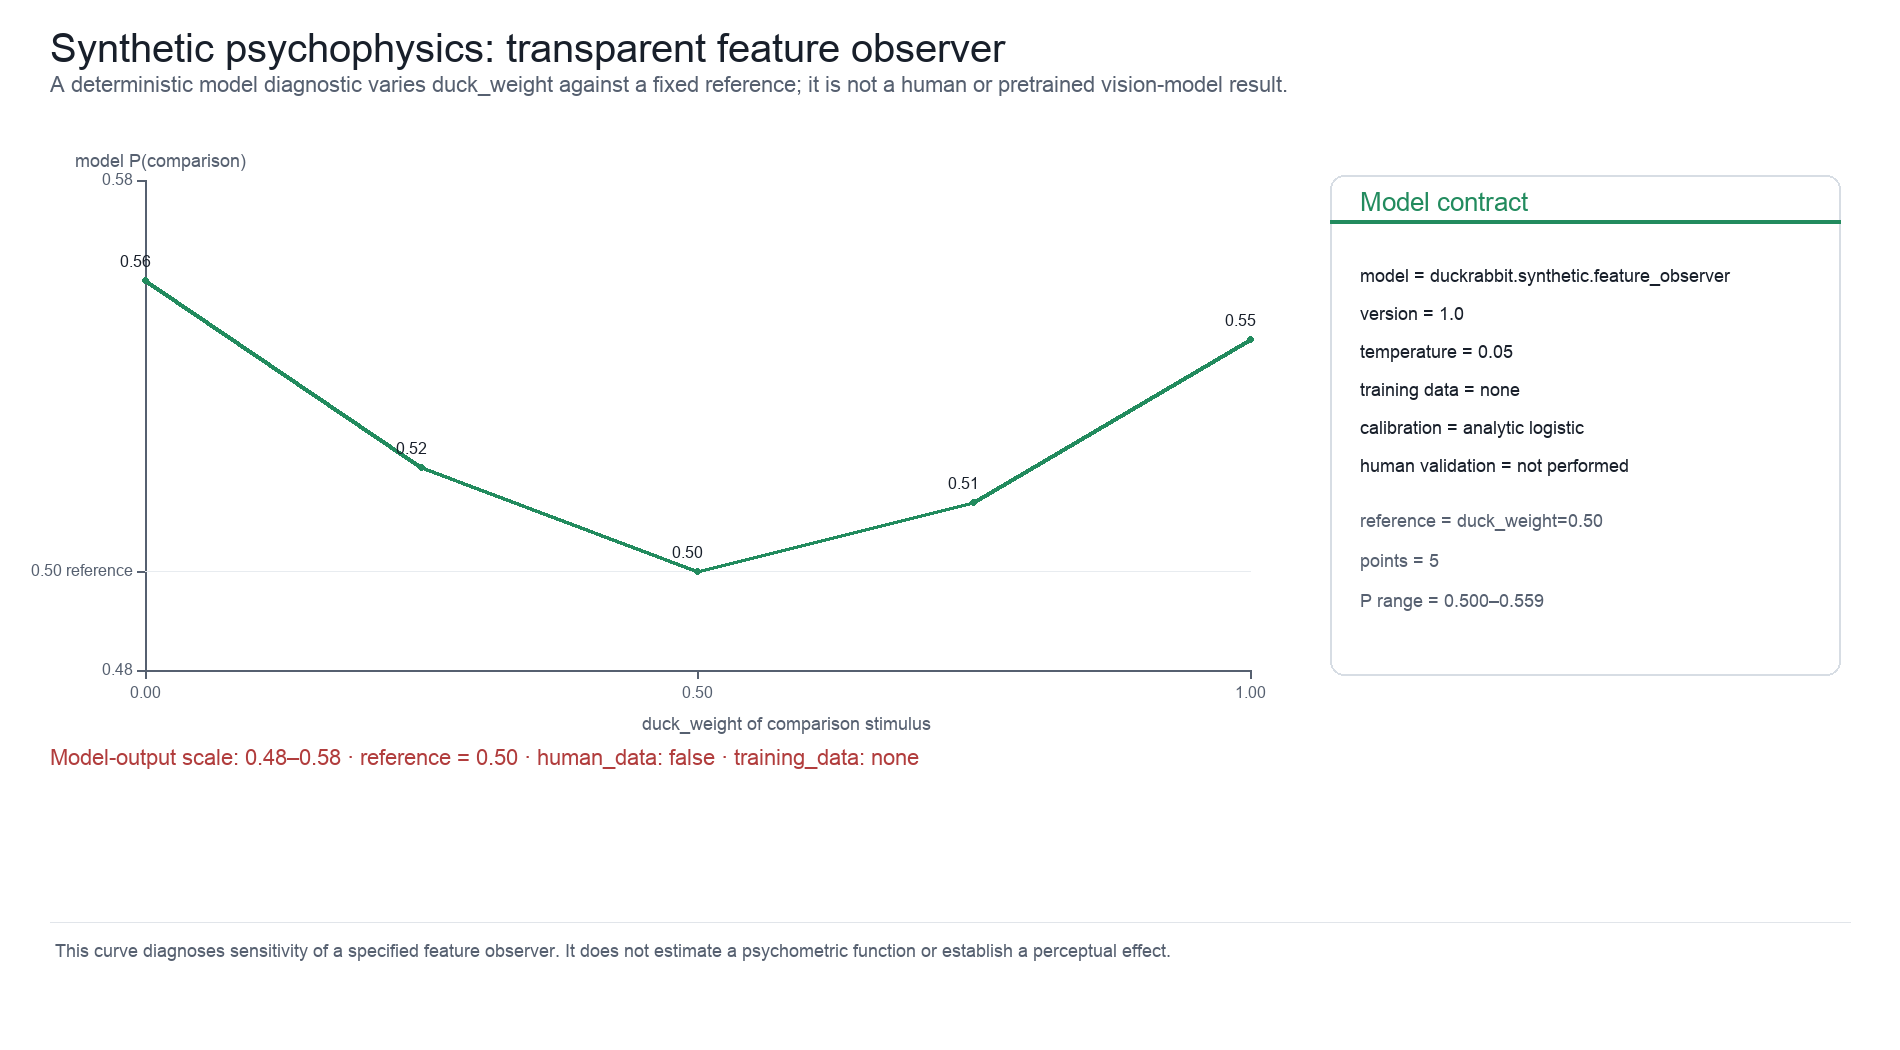
\includegraphics[keepaspectratio,alt={A narrow-range line plot shows deterministic model probability across duck\_weight values beside the model identity, temperature, no-training-data statement, and human-data boundary.}]{../figures/synthetic_psychophysics.png}}
\caption{A narrow-range line plot shows deterministic model probability
across duck\_weight values beside the model identity, temperature,
no-training-data statement, and human-data
boundary.}\label{fig:synthetic_psychophysics}
\end{figure}

What this figure shows: A narrow-range line plot shows deterministic
model probability across duck\_weight values beside the model identity,
temperature, no-training-data statement, and human-data boundary. The
hand-specified feature observer compares duck\_weight variants with a
fixed canonical reference. Its probability trace is computed
analytically from serialized features, weights, and temperature; source
data output/data/synthetic\_psychophysics.json records model ID/version,
reference and comparison digests, seed, calibration,
\breaktt{training\_data=none}, and \breaktt{human\_data=false}. The y-axis
is deliberately a narrow model-output range rather than a human
psychometric scale. Controls: duck\_weight comparison against fixed
reference; serialized feature weights and temperature; seed s=0.
Objective facts: model probability and score delta on the displayed
model-output scale; canonical stimulus digests; human\_data=false;
training\_data=none. Claim level: synthetic\_model\_output. Source data:
output/data/synthetic\_psychophysics.json (SHA-256 digest recorded in
the figure registry). Evidence lineage:
observer:preregistered\_estimands. Limitations: The model is
hand-specified, has no training data, has not been calibrated against
observers, and does not estimate a human threshold or effect size. Its
probabilities are model outputs, not participant responses or a
psychometric function. Boundary: This diagnostic tests deterministic
orchestration and metamorphic input-output behavior only; empirical
psychophysics remains future work.

The diagnostic fig.~\ref{fig:synthetic_psychophysics} evaluates a fully
serialized, hand-specified feature observer against a fixed canonical
reference while varying \texttt{duck\_weight}. Its logistic
probabilities are model outputs generated from explicit features,
weights, temperature, and seed; they are not a pretrained vision-model
score, a human psychometric function, an assumed human effect size, or
participant data. A future human study would require a preregistered
task, calibrated display and playback, consented participants, exclusion
and missingness rules, and an analysis contract before any observer
claim could be made.

\newpage

\section{Experimental and Computational
Setup}\label{sec:experimental_setup}

Core generation uses Python, NumPy, Pillow, and the standard library.
The default seed is 0 and generation is offline. The generators are
analytic in their typed parameters: the seed is recorded in manifests
and study plans but does not yet alter artifact bytes; seed-driven
stimulus randomization awaits a stochastic generator. PNG, GIF, WAV, and
NPZ are available without ffmpeg; MP4 and muxed audiovisual output
require both ffmpeg and ffprobe. Optional capabilities fail explicitly
rather than silently changing the requested artifact.

The deterministic validation suite executes real NumPy synthesis and
real temporary-file media round trips. It checks finite normalized
arrays, typed parameter boundaries, canonical hashes, dimensions,
channel layouts, sample rates, frame counts, timebases, duration
agreement, synchronization offsets, decoded stream facts, and
registry/evidence consistency.

This is a software-validation protocol, not a psychophysical experiment.
The tests establish repeatability under the declared software and
dependency conditions; they do not establish replicability of an
observer effect under a new display, playback chain, population, or
task. That distinction is why the release reports both the exact
environment contract and the missing observer evidence.

The publication workflow writes 15 scientific PNG figures plus a
separately provenance-recorded editorial cover, machine-readable
source-data sidecars, a typed figure registry, 10 markdown tables, and a
publication report. Each generated figure records its source function,
seed, caption, alt text, claim level, and SHA-256 digest. Generated
files are disposable; the tracked source is the generator and its tests.

The registry and cover report are independently revalidated after
generation. The registry validator rechecks code-owned captions,
evidence namespaces, source-data hashes, and figure hashes. The cover
validator rechecks the editorial source digest, portrait dimensions,
variant set, and delivery hashes. These checks prevent a successfully
rendered image from becoming an unexamined publication claim.

The observer harness is a data-free design layer. It creates
reproducibly randomized trial records, exports typed study plans,
generates synthetic responses for contract tests, and exposes model
templates. It does not collect or ship participant data. The publication
atlas additionally runs \breaktt{duckrabbit.synthetic.feature\_observer},
an explicitly hand-specified feature model with no training corpus. Its
canonical pairwise probabilities are serialized as model output and are
useful for end-to-end orchestration tests; they are not a real
vision-model estimate, a psychometric function, or an observer result.
Human sensitivity is deferred until a calibrated, consented,
preregistered study supplies response data and an analysis contract.

\newpage

\section{Reproducibility and Provenance}\label{sec:reproducibility}

The reproducibility contract is:

\begin{enumerate}
\def\labelenumi{\arabic{enumi}.}
\tightlist
\item
  construct the same frozen parameter dataclass;
\item
  use the same generator ID and the same deterministic seed;
\item
  compare the canonical artifact digest;
\item
  record the parameter schema, typed parameters, taxonomy, evidence
  boundary, canonical byte serialization, objective metrics, and
  encoding request;
\item
  if a file is written, inspect the decoded media and compare
  dimensions, channels, rates, frame counts, durations, timing offsets,
  and encoded hash;
\item
  retain the v2 manifest and source-data sidecars with the generated
  figure or table. Note that in this release the generators are analytic
  in their typed parameters: the request seed \emph{s} is recorded in
  manifests and study plans and excluded from the canonical digest, but
  it does not yet alter artifact bytes; seed-driven stimulus
  randomization awaits a stochastic generator.
\end{enumerate}

The contract is deliberately stronger than ``the file can be
downloaded.'' Research-software guidance treats versioned code,
executable procedures, dependencies, and retained inputs as part of the
reproducible object \citep{sandve2013simple, wilson2014bestpractices}.
FAIR guidance further asks that digital research objects be findable,
accessible, interoperable, and reusable, while noting that software has
lifecycle and maintenance constraints that are not identical to those of
static data \citep{wilkinson2016fair, lamprecht2020fairsoftware}.
DuckRabbit operationalizes those principles with typed metadata,
deterministic hashes, source-data sidecars, explicit licenses, and
release gates rather than by implying that a generated media file is a
complete scientific replication.

The package reports implemented, planned, input\_required as its catalog
status vocabulary and currently covers audio-visual, auditory, visual.
The evidence layer contains 18 entry records backed by 36 source
records, covering 18/18 catalog entries. The publication workflow
produces 15 figures and 10 tables from the live registry.

The public software record is
\href{https://github.com/docxology/DuckRabbit}{the DuckRabbit public
GitHub repository}, with Daniel Ari Friedman of the Active Inference
Institute as author. The release is archived on Zenodo at
\href{https://doi.org/10.5281/zenodo.21419693}{10.5281/zenodo.21419693}
(concept DOI, always resolves to the latest version), with
\href{https://doi.org/10.5281/zenodo.21419694}{10.5281/zenodo.21419694}
identifying this v0.5.0 release specifically.

The canonical buffer is the primary identity of a stimulus. Encoded
files are delivery artifacts with format-specific tolerances. The
observer protocol is a separate evidence layer: a manifest can prove
what was presented without proving what an observer experienced.

Synthetic psychophysics is a third, deliberately bounded object: the
model is a hand-specified deterministic feature observer; no training
data; human\_data=false, registered as
\breaktt{duckrabbit.synthetic.feature\_observer}. The model version,
feature schema, weights, temperature, seed, calibration statement,
canonical reference/comparison digests, and \breaktt{human\_data=false}
flag are retained in \breaktt{output/data/synthetic\_psychophysics.json}.
Re-running this diagnostic checks deterministic model orchestration and
stimulus-feature sensitivity; it does not estimate a human observer or
replace empirical psychophysics.

The v2 verifier is a relational check rather than a field-presence
check. It rejects summaries whose dimensions, dtype, byte count, rates,
duration, signal range, frame deltas, or signed audiovisual offset
disagree. Public manifest and inspection mappings are recursively frozen
after validation, and rational frame rates are reduced before entering
the clock contract. The read-only capability probe records whether
Pillow, NumPy, ffmpeg, or ffprobe are available in the current
environment; unavailable delivery paths remain explicit rather than
being silently downgraded.

The minimal regeneration commands are:

\begin{Shaded}
\begin{Highlighting}[]
\ExtensionTok{uv}\NormalTok{ run pytest }\AttributeTok{{-}q} \AttributeTok{{-}{-}cov}\OperatorTok{=}\NormalTok{src/duckrabbit }\AttributeTok{{-}{-}cov{-}fail{-}under}\OperatorTok{=}\NormalTok{90}
\ExtensionTok{uv}\NormalTok{ run python scripts/generate\_publication\_outputs.py}
\ExtensionTok{uv}\NormalTok{ run python scripts/generate\_manuscript\_variables.py}
\end{Highlighting}
\end{Shaded}

\subsection{Data availability and software
citation}\label{data-availability-and-software-citation}

No participant records, fitted observer coefficients, or human
psychophysics are bundled. The synthetic diagnostic is explicitly model
output with \breaktt{human\_data=false} and \breaktt{training\_data=none}.
Reuse should cite Daniel Ari Friedman and the release metadata in
\texttt{CITATION.cff}, together with the source-specific scholarship in
\texttt{references.bib}. Software-citation principles recommend citing
the software object itself, with enough version and identity information
to distinguish one release from another \citep{smith2016software}. The
DOI field carries the real, minted concept DOI
(\breaktt{10.5281/zenodo.21419693}) and \texttt{doi\_status} is
\texttt{published}; no resolver URL was manufactured before that
identifier existed.

\newpage

\section{Scope, Related Work, and Limitations}\label{sec:scope}

\subsection{Scope and epistemic
boundary}\label{scope-and-epistemic-boundary}

DuckRabbit is a typed, reproducible stimulus-construction platform. Its
unit of work is an immutable request that yields a canonical image,
audio buffer, video sequence, or audiovisual timeline, together with
objective measurements and provenance. It is not an exhaustive ontology
of all illusions, a perceptual theory, a participant database, or a
substitute for a controlled psychophysics experiment. The live registry
is therefore a deliberately bounded catalog: it enumerates the families
for which this release has both a generator contract and a stated
evidence boundary. Appendix A gives the complete current matrix; the
absence of a family from that matrix is not a claim that the family is
unimportant or unsupported in the wider literature.

The central distinction is between a construction and an observation. A
DuckRabbit generator can establish the dimensions, pixel values, sample
values, frequency components, frame clock, declared synchronization
offset, encoded hash, and decoded media facts of its output. It cannot,
from those facts alone, establish what a person sees, hears, counts,
localizes, groups, or reports. Every figure caption, evidence record,
and claim-ledger entry preserves this boundary. In particular, a
literature citation establishes a source-supported statement about a
stimulus family or result under that source's conditions; it does not
certify pixel- or task-identical replication by a DuckRabbit artifact.

The historical foundation is intentionally worldwide and layered. The
package does not present a single invention narrative: it places ancient
Greek, medieval Arabic, classical Chinese, and early-modern European
sources beside nineteenth-century psychophysics and modern experimental
work. This is a scholarly orientation for separating physical
construction, interpretation, and observer evidence; it is not a claim
that the current source set exhausts the visual, auditory, or perceptual
traditions of any region.

\subsection{Visual families}\label{visual-families}

The modern label ``visual illusion'' sits on a longer experimental
history than the package's contemporary review sources alone suggest.
Oppel's mid-century catalogue of geometrical-optical illusions is now
accessible with translation and commentary \citep{wade2017oppel}, and
the primary nineteenth-century records include Zöllner's account of
crossing-line distortions and Müller-Lyer's report of the arrow-wing
configuration \citep{zoellner1860pseudoscopy, mullerlyer1889optical}.
These sources are treated as historical anchors, not as evidence that a
present-day raster is identical to an original plate or that its
observer effect is invariant across conditions.

Gregory's classification is useful as a historical and conceptual
orientation, but it is not a universally agreed ontology. DuckRabbit
consequently stores visual modality, mechanism, perceptual signature,
stimulus requirements, and evidence status as separate facets rather
than treating a single label as an explanation
\citep{gregory1997visual}. The visual atlas covers the implemented
families currently registered in the package: ambiguous figure,
contrast, apparent motion, Müller-Lyer, Poggendorff, Ponzo, Kanizsa-type
subjective contour, Ebbinghaus contextual size, and Zöllner/Judd
orientation-related geometry. ``Coverage'' here means one deterministic
representative per live entry, not a claim that one raster captures the
historical stimulus space.

The duck/rabbit construction is an explicit example of why that
distinction matters. Brugger's historical analysis discusses variation
among figure variants and observers; DuckRabbit therefore exposes a
blend parameter and labels its output as a construction rather than
promising a fixed alternation rate or universal bistability
\citep{brugger1999duckrabbit}. The Müller-Lyer entry uses typed arrow
geometry. Its engineering form is compatible with a family whose image
statistics have been analyzed as potentially informative about
image-source relationships, but the implementation does not adjudicate
that account or infer a perceived-length report
\citep{mullerlyer1889optical, howe2005muller}.

The Poggendorff generator makes the occluding geometry and virtual-line
orientation explicit. This is appropriate to a literature in which
orientation estimation and filtering accounts are theoretically
relevant, while avoiding the stronger claim that a particular raster
reproduces a published bias without the same observers, viewing
conditions, and response task \citep{morgan1999poggendorff}. The Ponzo
construction is similarly bounded: the converging context and test bars
are deterministic, whereas the literature contains multiple explanations
of Ponzo-like effects rather than one settled mechanism
\citep{fisher1967ponzo, yildiz2022ponzo}.

Kanizsa-style subjective contours are represented as an illusory-contour
construction with explicit inducer geometry. The historical account
motivates the family label, while modern reviews place contour
completion within a wider literature on grouping, figure-ground
organization, attention, and neural mechanisms
\citep{kanizsa1976contours, wagemans2012gestalt}. Neither source
licenses a claim that the generated mask produces a uniform contour
percept across observers. The Ebbinghaus entry controls target and
surround geometry; classic work demonstrates that judged size depends on
context, contour, and comparison conditions, while later work shows that
motion and other parameters can alter the effect
\citep{weintraub1979ebbinghaus, mruczek2015ebbinghaus}. DuckRabbit's
static default is therefore an engineering baseline rather than a
task-identical replication. Zöllner/Judd geometry is likewise retained
as a source-linked line arrangement. Zöllner's 1860 report supplies the
historical primary anchor, while later work supplies a modern analysis
of spatial filtering \citep{zoellner1860pseudoscopy, earle1995zollner}.
Its typed line lengths and orientations make the spatial stimulus
auditable, while orientation judgments remain outside the package
contract.

Finally, apparent motion is included in the visual coverage panel
because its defining engineering object is temporal succession, not
merely a static pattern. The package verifies frame order, frame rate,
timestamps, and frame-to-frame differences. Wertheimer's foundational
work and Sekuler's later analysis motivate the family distinction;
neither source turns a generated frame strip into a universal report of
motion \citep{wertheimer1912motion, sekuler1996wertheimer}.

\subsection{Auditory families}\label{auditory-families}

The auditory catalog separates harmonic construction, spectral
completion, pitch-class context, dichotic channel assignment, and
continuity/masking. A Shepard-like signal is represented through
additive partials and explicit envelopes, following a historical
literature of tone psychology and later work on assimilation to an
internalized musical scale
\citep{stumpf1883tonpsychology, shepard1984scale}. The canonical buffer
exposes sample rate, amplitude bounds, channel count, partial
frequencies, and envelope parameters. It does not determine a listener's
perceived pitch height or direction.

The missing-fundamental construction removes a low component while
retaining harmonically related partials. This makes the spectral
condition reproducible; the associated pitch interpretation remains a
listener-level question \citep{zatorre2005missing}. Tritone and octave
entries preserve channel structure, phase, frequency relationships, and
timing in typed parameters. Deutsch's foundational accounts and Repp's
analysis of spectral-envelope and context effects motivate the evidence
records, while also making listener and context dependence central
limitations
\citep{deutsch1986tritone, repp1997tritone, deutsch1974octave}.

Auditory continuity is represented as an interrupted target with a typed
masker and gap. Warren's classic perceptual-restoration result and
Riecke and colleagues' separation of sensory and decisional
contributions justify the family's inclusion, but a generated masker is
not evidence that a listener will report an uninterrupted sound
\citep{warren1970continuity, riecke2011continuity}. The audio atlas
therefore reports RMS, peak, spectral centroid, bandwidth, channel
layout, and exact sample-level provenance---not continuity, pitch, or
stream judgments.

\subsection{Audiovisual and temporal binding
families}\label{audiovisual-and-temporal-binding-families}

Audiovisual constructions require a shared clock and an explicit sign
convention for offsets. The sound-induced-flash entry creates a typed
visual event and one or more audio events; the evidence record links it
to the primary demonstration and to a review of the broader literature
\citep{shams2000sifi, hirst2020sound}. The package can verify event
timestamps, sample/frame clocks, and declared offsets. It does not infer
a reported flash count, and it does not assume that the same temporal
window applies across displays, headphones, latencies, or observers.

The spatial ventriloquist construction treats spatial discrepancy as a
parameter and records the channel and display requirements. Reviews
describe the ventriloquist illusion as a tool for studying multisensory
processing, but the review's scope is not a license to claim spatial
capture from a file alone \citep{bruns2019ventriloquist}. More general
audiovisual accounts describe integration and segregation as a
causal-inference problem shaped by temporal regularities and signal
reliability \citep{noppeney2018causal}. That framework clarifies why a
declared offset is an experimental input, not an observer-level outcome.
Temporal ventriloquism receives a separate temporal-binding signature
rather than being collapsed into spatial capture. Vroomen and de Gelder
manipulated sound--flash timing in a flash-lag task and reported
timing-dependent changes under those experimental conditions;
Hartcher-O'Brien and Alais studied temporal ventriloquism in a purely
temporal context
\citep{vroomen2004temporal, hartcherobrien2011temporal}. DuckRabbit
implements the stimulus-side timing contract and leaves the
observer-side temporal-recalibration estimate to a future study.

McGurk remains \texttt{input\_required}. The classic speech study
motivates the family, but a lawful and reproducible implementation
requires checksummed speech and video fixtures, licensing or consent
records, a precise preprocessing contract, and an ethical validation
protocol \citep{mcgurk1976speech}. Cataloguing the gap is more
informative than silently substituting an unrelated synthetic voice or
claiming that a generic audiovisual mismatch is a McGurk replication.

\subsection{From literature to engineering
contract}\label{from-literature-to-engineering-contract}

For each entry, the evidence matrix records a source role, exact
source-supported claim, engineering basis, limitation, and audit status.
The roles distinguish primary demonstration, review or synthesis,
theoretical account, engineering basis, limitation, and input gap. This
prevents three common category errors: treating a theory as settled
mechanism, treating a review as validation of new code, and treating a
generator's deterministic output as a participant result.

The package's literature fidelity is therefore best described as
``family-linked, parameterized engineering construction.'' Some defaults
are historically motivated; none should be read as a claim of pixel
identity unless that identity is separately established. The checked-in
scholarship snapshot provides offline structural validation, including
citation-key and DOI/URL format checks. The explicit network audit adds
resolver observations and metadata matching; reachability alone is not
treated as bibliographic verification. This is a reproducible evidence
boundary, not a claim that every source is equally accessible or that
theoretical disputes have been resolved.

\subsection{Limitations and future observer
work}\label{limitations-and-future-observer-work}

The package does not claim clinical validity, universal effect sizes,
cross-cultural invariance, perceptual equivalence across displays or
headphones, or observer-level truth from objective media metrics.
Playback level, gamma and display calibration, viewing distance, refresh
rate, stereo separation, room acoustics, audio transducer response,
attention, expectation, language, expertise, and task can all matter.
Codec behavior and device latency can introduce additional differences
even when decoded media facts match within the declared tolerance.

The synthetic observer diagnostic is intentionally not a substitute for
a real vision model or human data. It is a serialized, hand-specified
feature function with \breaktt{training\_data=none},
\breaktt{calibration\ =\ analytic}, and \breaktt{human\_data=false}; its
metamorphic and sensitivity checks test orchestration, not visual
consciousness or human discrimination. A future observer study must
pre-register the response scale, reference condition, estimand,
exclusions, missing-data rule, randomization seed, display and playback
controls, and uncertainty procedure. It must also report the participant
and item sampling frame rather than importing a model-output probability
as an assumed effect size. The observer harness is consequently
study-ready scaffolding, not a result set.

No participant data are bundled with DuckRabbit. The data-availability
boundary is intentional: canonical artifacts, encoded fixtures where
lawful, source-data sidecars, and deterministic synthetic diagnostics
are software outputs; observer outcomes require separately governed data
collection. The package is authored by Daniel Ari Friedman and is
archived under DOI \breaktt{10.5281/zenodo.21419693}; release metadata
and software-citation guidance are generated from the same identity
contract as the manuscript.

\newpage

\section{Publication Atlas, Caption Contract, and Scholarship
Audit}\label{sec:publication_audit}

The publication layer is generated from the same typed package state as
the stimuli. It contains 15 scientific figures, 10 machine-readable
tables, and a separately provenance-recorded editorial cover. The cover
is an illustration of the project's subject and methods aesthetic; it is
not a stimulus, a participant result, or evidence of a perceptual
effect.

\subsection{Claim-level visualization}\label{claim-level-visualization}

\begin{figure}
\centering
\pandocbounded{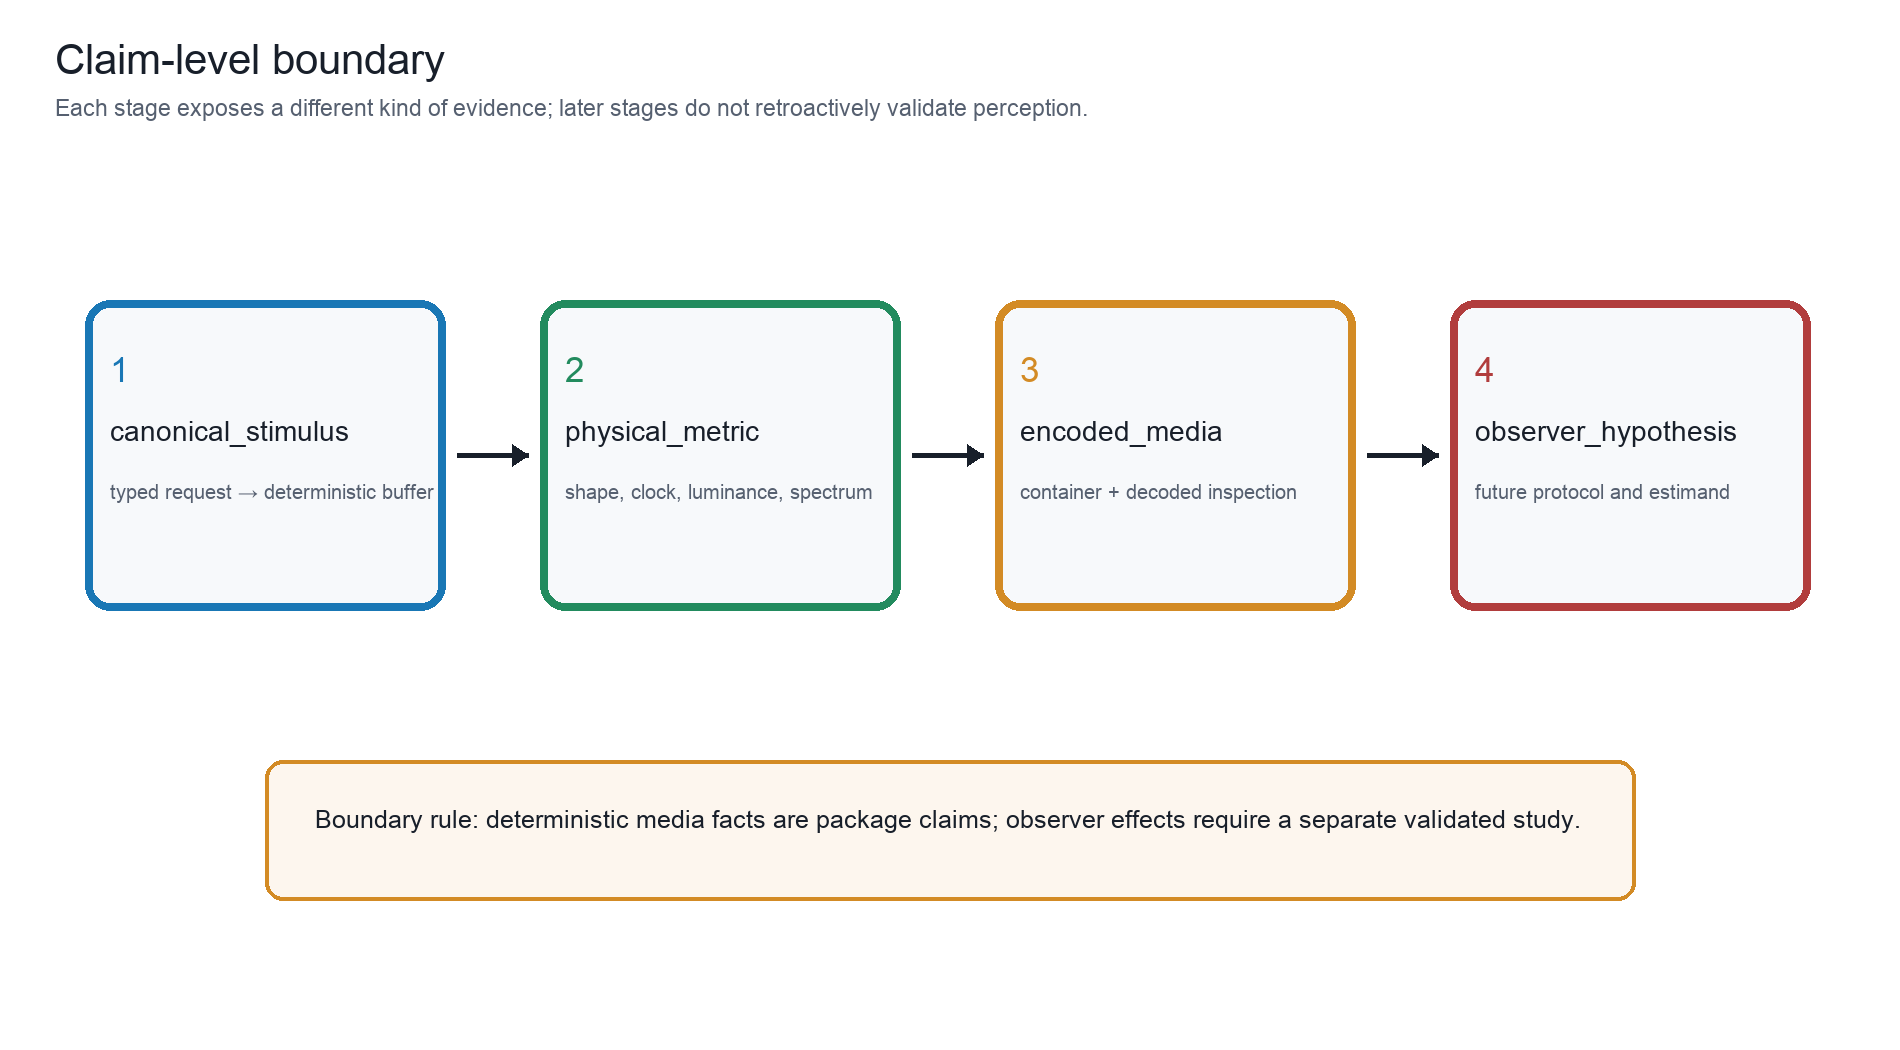
\includegraphics[keepaspectratio,alt={Four numbered boxes separate canonical stimulus, physical metric, encoded media, and observer hypothesis, with a boundary rule stating that observer effects require a separate study.}]{../figures/claim_boundary.png}}
\caption{Four numbered boxes separate canonical stimulus, physical
metric, encoded media, and observer hypothesis, with a boundary rule
stating that observer effects require a separate
study.}\label{fig:claim_boundary}
\end{figure}

What this figure shows: Four numbered boxes separate canonical stimulus,
physical metric, encoded media, and observer hypothesis, with a boundary
rule stating that observer effects require a separate study. The
four-stage boundary distinguishes what DuckRabbit can establish
directly---canonical stimulus identity, physical/media metrics, and
decoded encoded-media facts---from a future observer hypothesis. Source
data output/data/claim\_boundary.json records the stage definitions and
boundary rule; the arrows describe increasing evidential requirements,
not an inference that one stage establishes the next. Controls: claim
levels in the taxonomy and manifest; seed not applicable to the
explanatory diagram. Objective facts: no unit-bearing objective quantity
is applicable; stage definitions and evidence boundaries are preserved
in the sidecar. Claim level: source\_supported. Source data:
output/data/claim\_boundary.json (SHA-256 digest recorded in the figure
registry). Evidence lineage: formalism:eq:observer\_estimand,
formalism:eq:canonical\_digest. Limitations: The diagram is a
documentation contract and does not replace a preregistered observer
study or empirical data. Boundary: A deterministic artifact can support
a future hypothesis but cannot supply the observer data required to test
it.

The claim boundary in fig.~\ref{fig:claim_boundary} is a typed epistemic
interface. A canonical digest identifies a deterministic buffer;
objective metrics identify properties of that buffer; encoded-media
verification identifies facts of the delivered file. A future observer
hypothesis is a different object with its own protocol, estimand, and
uncertainty interval.

\subsection{Scholarship map and
lineage}\label{scholarship-map-and-lineage}

\begin{figure}
\centering
\pandocbounded{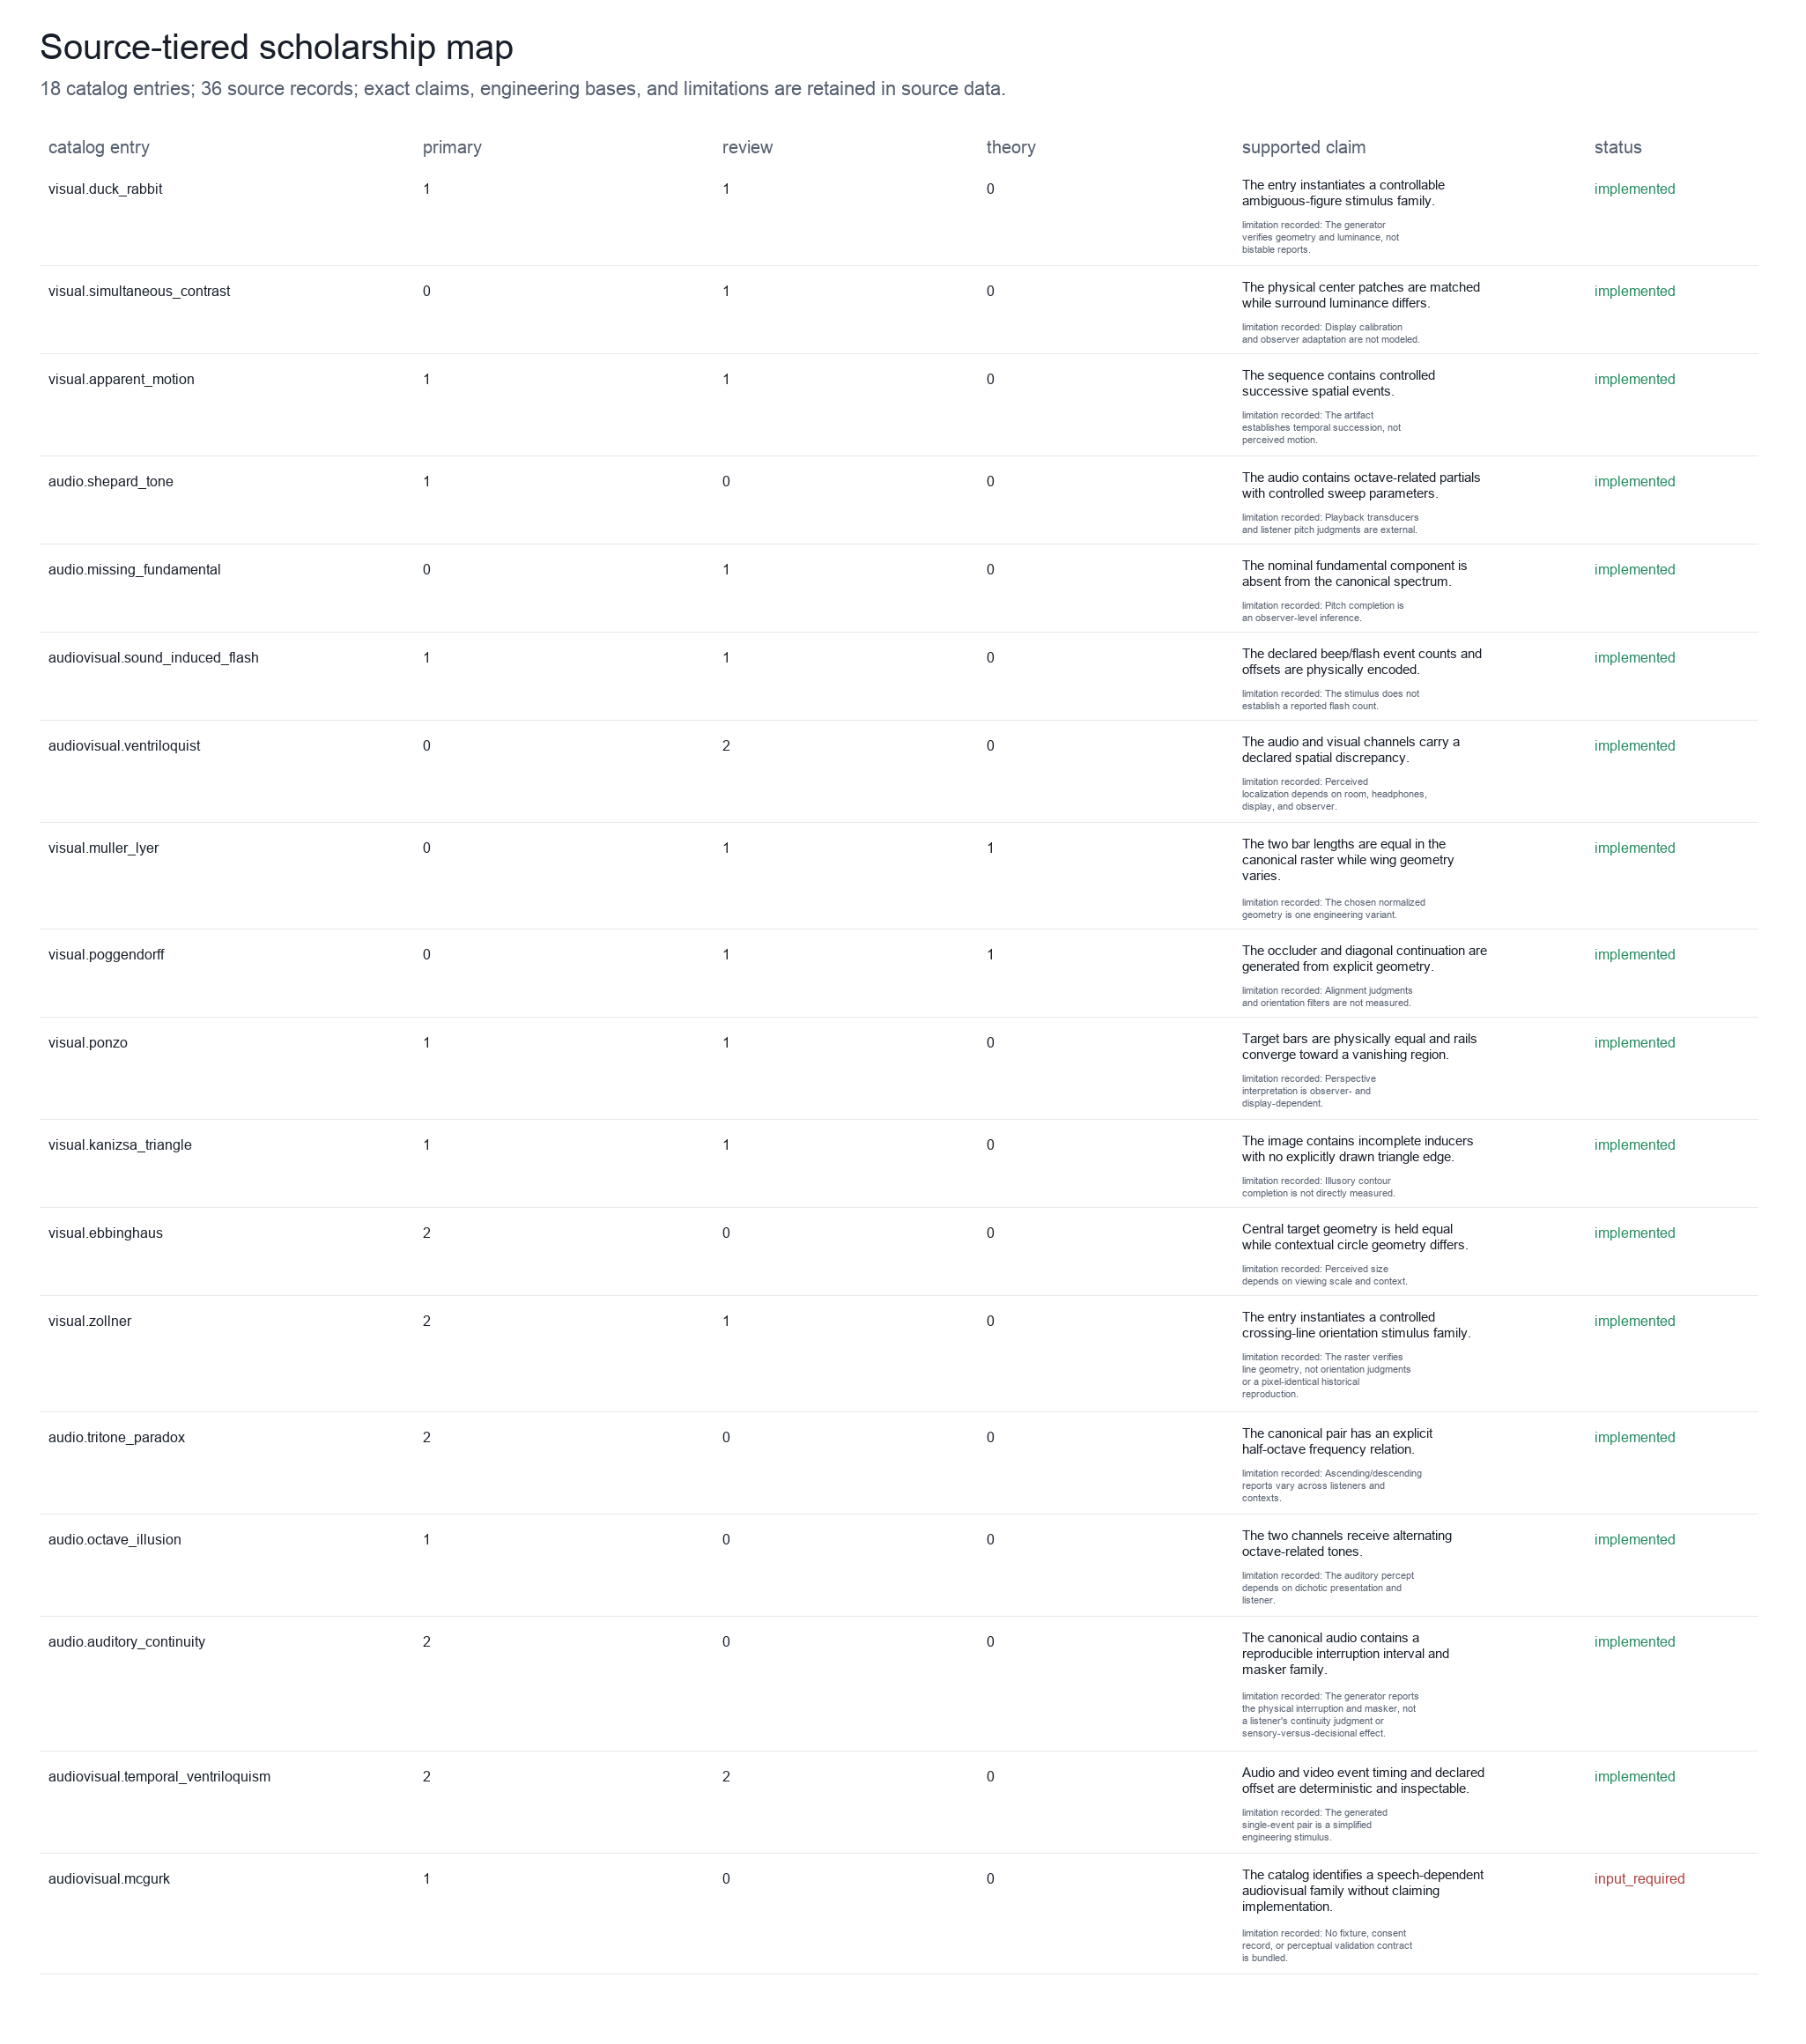
\includegraphics[keepaspectratio,alt={Rows map catalog entries to source tiers, exact supported claims, engineering bases, limitations, and implementation status.}]{../figures/scholarship_map.png}}
\caption{Rows map catalog entries to source tiers, exact supported
claims, engineering bases, limitations, and implementation
status.}\label{fig:scholarship_map}
\end{figure}

What this figure shows: Rows map catalog entries to source tiers, exact
supported claims, engineering bases, limitations, and implementation
status. The map links every catalog entry to its primary, review, and
theory records, then preserves the exact source-supported claim,
engineering departure, limitation, and implementation status. Source
data output/data/scholarship\_map.json are generated from the checked-in
evidence matrix; a source record supports only the statement written in
that record and does not certify pixel- or task-identical replication.
Controls: checked-in evidence matrix; source roles and entry statuses;
audit date recorded in data/evidence\_matrix.json. Objective facts: one
evidence row per catalog entry (18 entries); source-tier counts, exact
claim text, engineering basis, limitation, and gap status. Claim level:
source\_supported. Source data: output/data/scholarship\_map.json
(SHA-256 digest recorded in the figure registry). Evidence lineage:
gregory1997visual, brugger1999duckrabbit, yildiz2022ponzo,
hirst2020sound, bruns2019ventriloquist. Limitations: The offline
snapshot validates citation and lineage structure; live resolver status
is a separate audit, and classifications can remain contested. Boundary:
Scholarship coverage bounds the package's evidence record and does not
establish that any generated stimulus produces a universal percept.

The source map fig.~\ref{fig:scholarship_map} and
tbl.~\ref{tbl:evidence_audit} make five distinctions explicit: a primary
demonstration, a review, a theoretical account, DuckRabbit's engineering
basis, and an evidence limitation. Brugger's duck/rabbit study documents
variation across figure variants and observers; this supports a careful
ambiguity-family record, not a universal bistability claim
\citep{brugger1999duckrabbit}. Yildiz et al.~review competing
explanations of Ponzo-like illusions, so the catalog retains both a
geometric construction and an unresolved theoretical boundary
\citep{yildiz2022ponzo}. Repp's tritone analysis likewise motivates
listener- and context-sensitive limitations \citep{repp1997tritone}.

The audit also treats software and its metadata as part of the scholarly
record. FAIR guidance emphasizes machine-actionable provenance and
reuse, and software-citation principles emphasize crediting an
identifiable version rather than citing an undifferentiated project name
\citep{wilkinson2016fair, smith2016software}. Accordingly, the release
includes \texttt{CITATION.cff}, CodeMeta, Zenodo metadata, versioned
manifests, source-data sidecars, and resolver-linked bibliography
entries. These improve discoverability and attribution; they do not
increase the evidential level of any perceptual claim.

The public software identity is explicit: DuckRabbit is published and
citable at the \href{https://github.com/docxology/DuckRabbit}{DuckRabbit
public GitHub repository} under the authorship of Daniel Ari Friedman,
Active Inference Institute. The generated bundle in this repository
remains the authoritative release candidate until the external template
handoff is completed.

\subsection{Formal traceability and objective
metrics}\label{formal-traceability-and-objective-metrics}

\begin{figure}
\centering
\pandocbounded{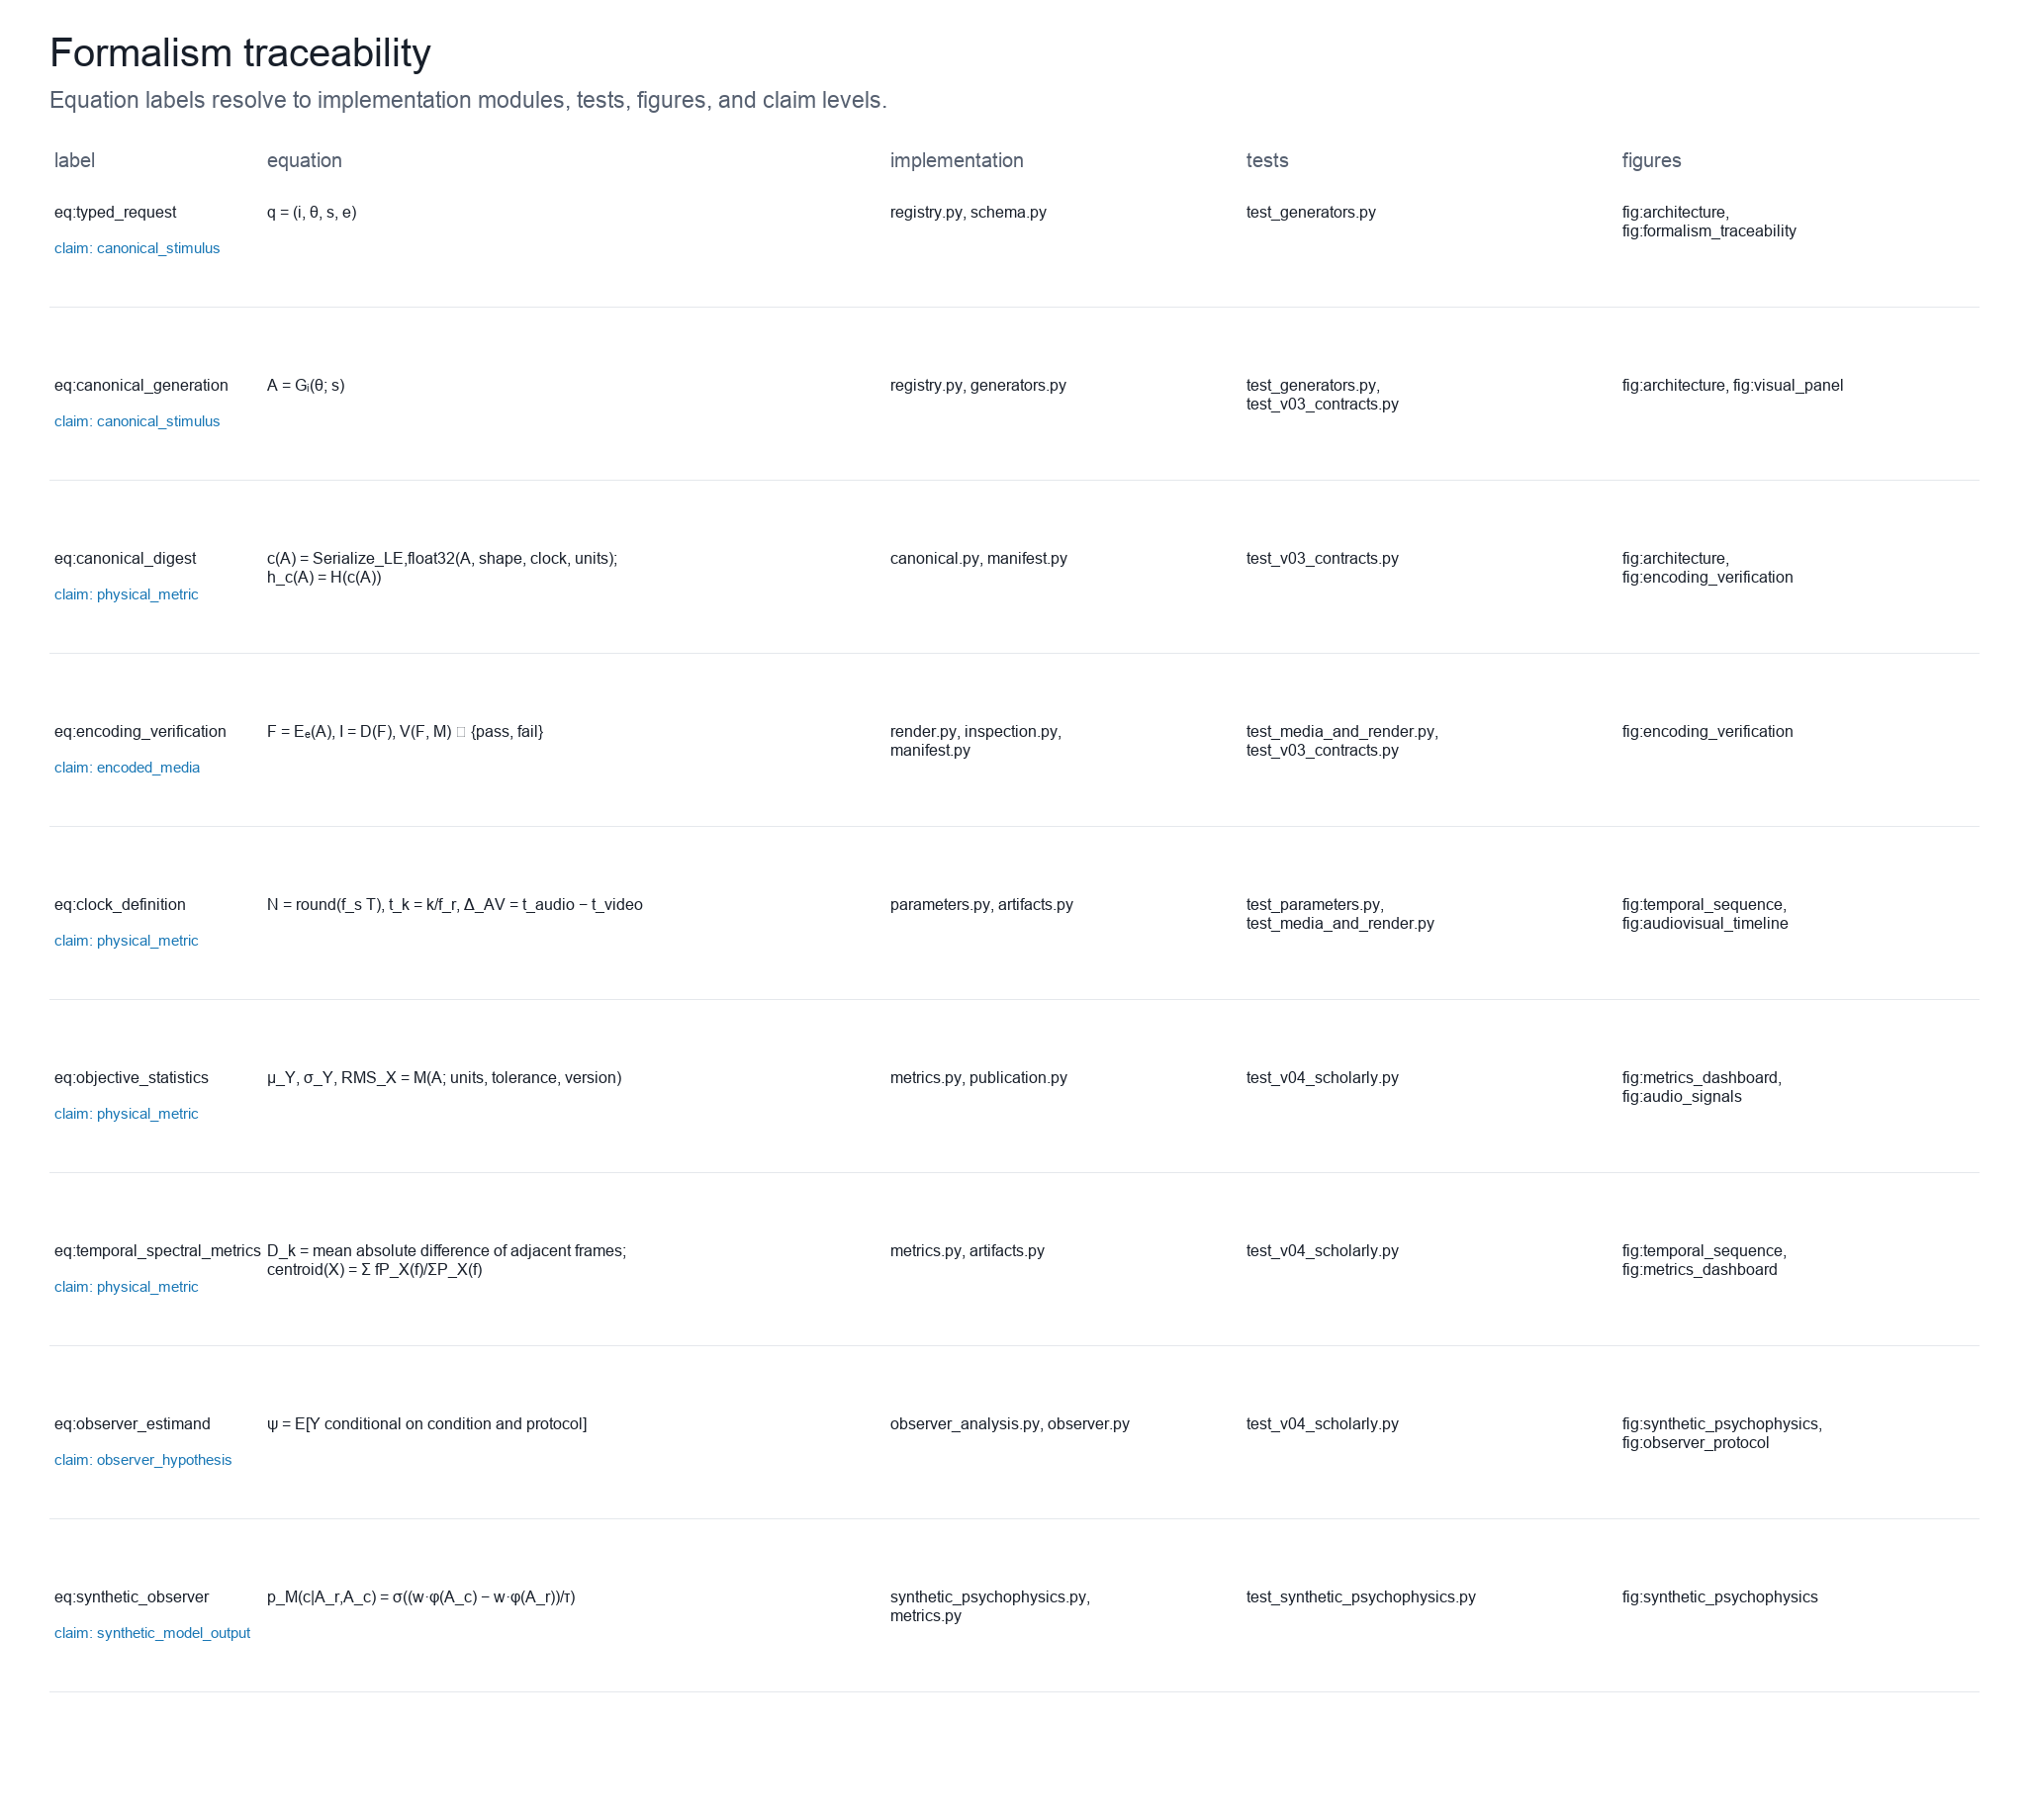
\includegraphics[keepaspectratio,alt={Rows connect equation labels to their mathematical definition, implementation paths, tests, figure labels, and claim levels.}]{../figures/formalism_traceability.png}}
\caption{Rows connect equation labels to their mathematical definition,
implementation paths, tests, figure labels, and claim
levels.}\label{fig:formalism_traceability}
\end{figure}

What this figure shows: Rows connect equation labels to their
mathematical definition, implementation paths, tests, figure labels, and
claim levels. The traceability registry connects the nine numbered
equations to symbols, implementation modules, tests, and registered
figures. Source data output/data/formalism\_traceability.json is the
machine-readable crosswalk used by the manuscript; it demonstrates
contract coverage and test linkage without converting formal notation
into empirical evidence. Controls: formalism registry version; seed not
applicable to the traceability diagram. Objective facts: nine equation
records with implementation, test, figure, and claim-level fields; no
unit-bearing measurement is plotted. Claim level: physical\_metric.
Source data: output/data/formalism\_traceability.json (SHA-256 digest
recorded in the figure registry). Evidence lineage:
formalism:eq:canonical\_digest, formalism:eq:clock\_definition,
formalism:eq:objective\_statistics. Limitations: Traceability records
documentation and verification scope; it does not establish the truth of
an observer-level theory. Boundary: A linked equation and test can show
an implemented contract, not a validated perceptual law.

The formalism registry fig.~\ref{fig:formalism_traceability} links
equations
eqns.~\ref{eq:typed_request}, \ref{eq:canonical_generation}, \ref{eq:canonical_digest}, \ref{eq:encoding_verification}, \ref{eq:clock_definition}, \ref{eq:objective_statistics}, \ref{eq:temporal_spectral_metrics}, \ref{eq:observer_estimand}, \ref{eq:synthetic_observer}
to implementation modules, tests, and figures. The contract is
intentionally auditable: equation labels point to code-owned records,
while empirical claims remain outside the generator's authority.

\begin{figure}
\centering
\pandocbounded{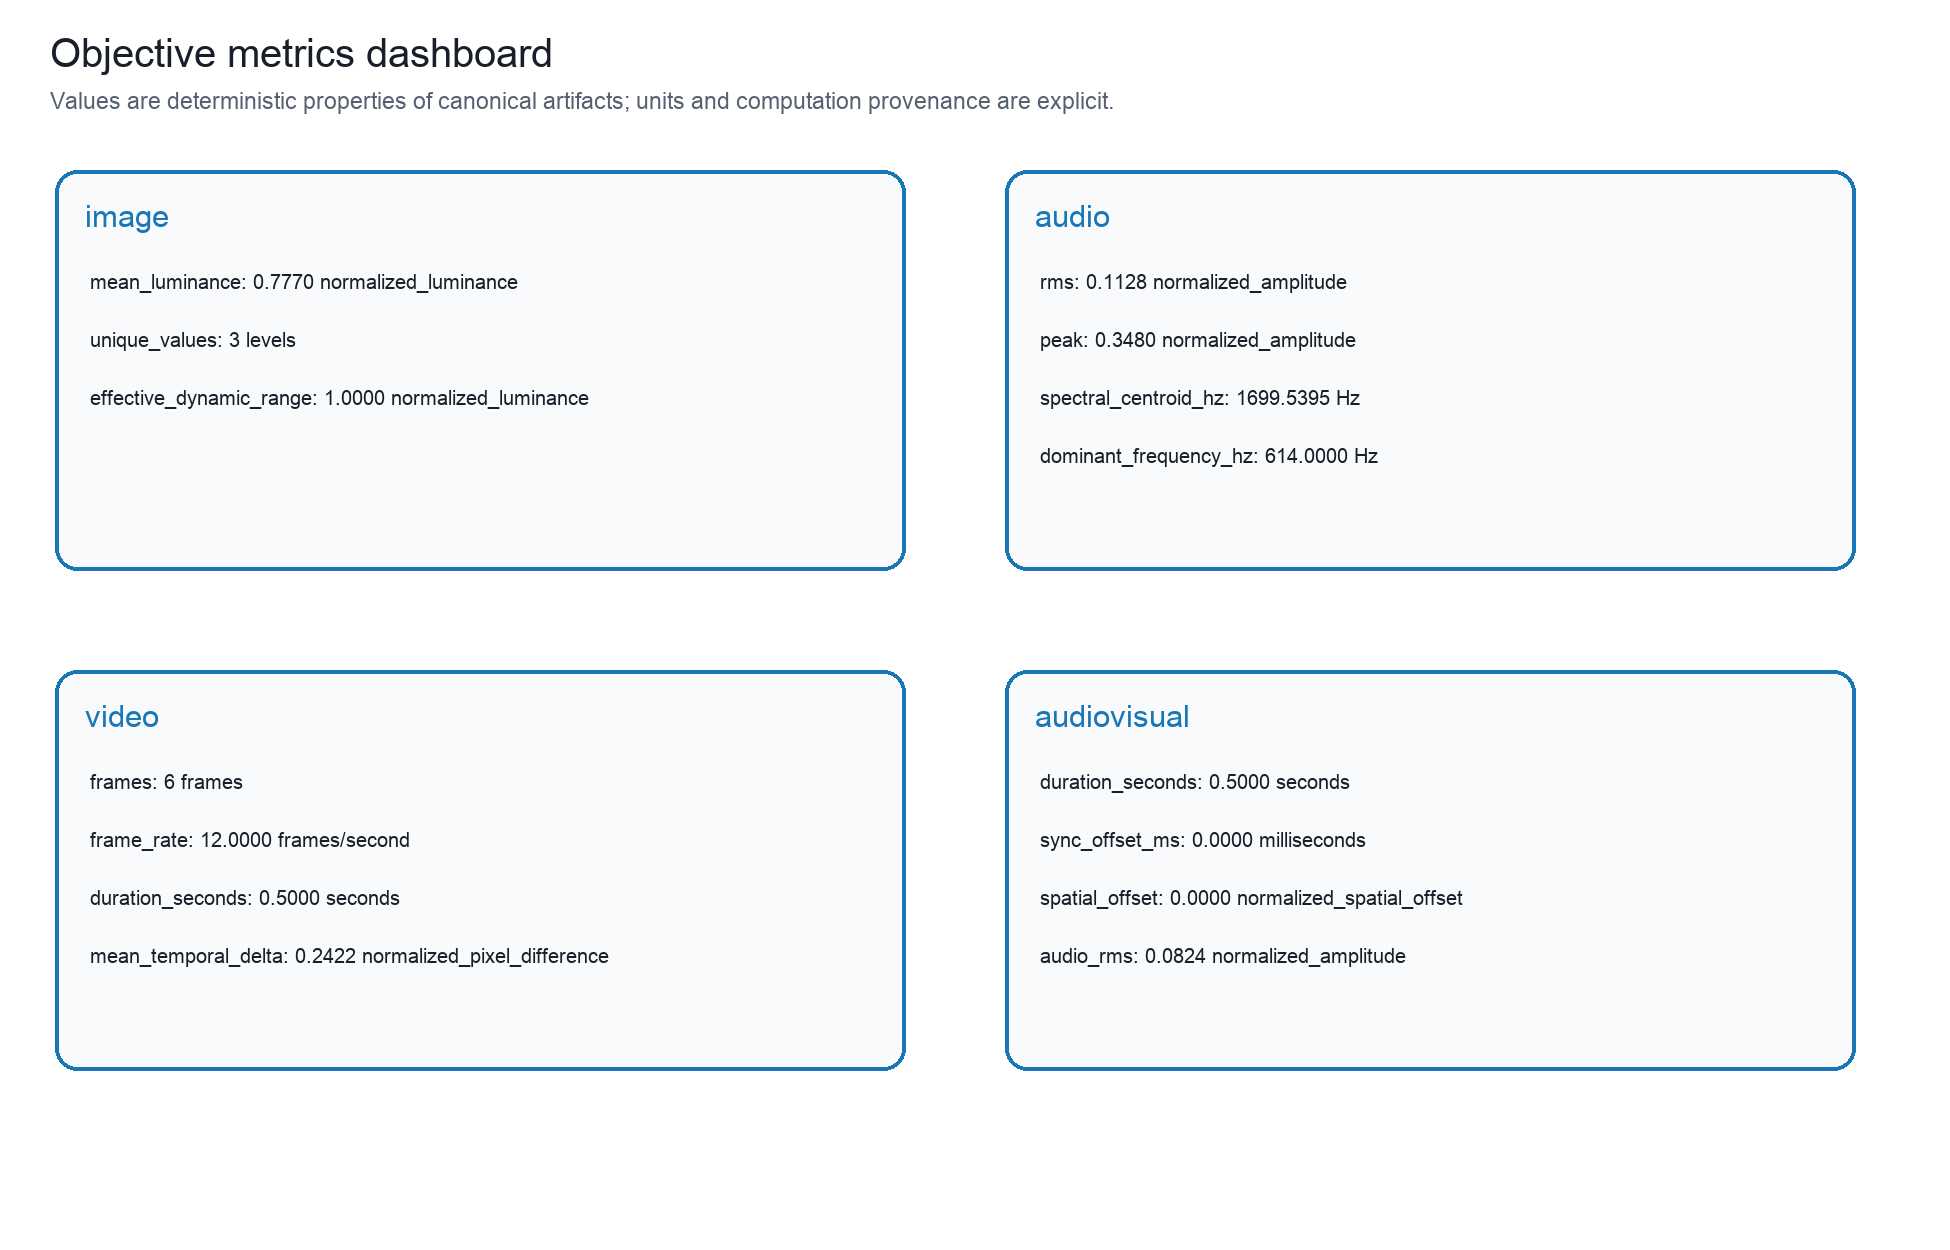
\includegraphics[keepaspectratio,alt={Four artifact cards list image, audio, video, and audiovisual metrics with units, computation provenance, and claim level.}]{../figures/metrics_dashboard.png}}
\caption{Four artifact cards list image, audio, video, and audiovisual
metrics with units, computation provenance, and claim
level.}\label{fig:metrics_dashboard}
\end{figure}

What this figure shows: Four artifact cards list image, audio, video,
and audiovisual metrics with units, computation provenance, and claim
level. The dashboard presents representative measurements from image,
audio, video, and audiovisual canonical artifacts. Source data
output/data/metrics\_dashboard.json retains metric name, value, unit,
computation version, tolerance, claim level, and canonical digest;
luminance is normalized, amplitude is normalized, spectra are in hertz,
frame differences are normalized pixel differences, and synchronization
is in milliseconds. Controls: default canonical artifacts; metric
computation version and tolerance recorded in the source-data sidecar;
seed s=0. Objective facts: finite objective values with units:
normalized luminance/amplitude, Hz, normalized pixel difference, ms,
counts, and durations. Claim level: physical\_metric. Source data:
output/data/metrics\_dashboard.json (SHA-256 digest recorded in the
figure registry). Evidence lineage: formalism:eq:objective\_statistics,
formalism:eq:temporal\_spectral\_metrics. Limitations: Metrics are media
properties and do not encode pitch, size, motion, localization, binding,
or other observer interpretations. Boundary: Metric reproducibility is a
package property; interpretation as perception requires a separate
observer design and data.

The metrics dashboard fig.~\ref{fig:metrics_dashboard} reports units,
computation version, and canonical digests. Luminance statistics are
normalized raster properties; RMS and peak are normalized-amplitude
properties; spectral values are in Hz; frame deltas are normalized pixel
differences; and synchronization offsets are in milliseconds. None is a
psychophysical score.

\begin{figure}
\centering
\pandocbounded{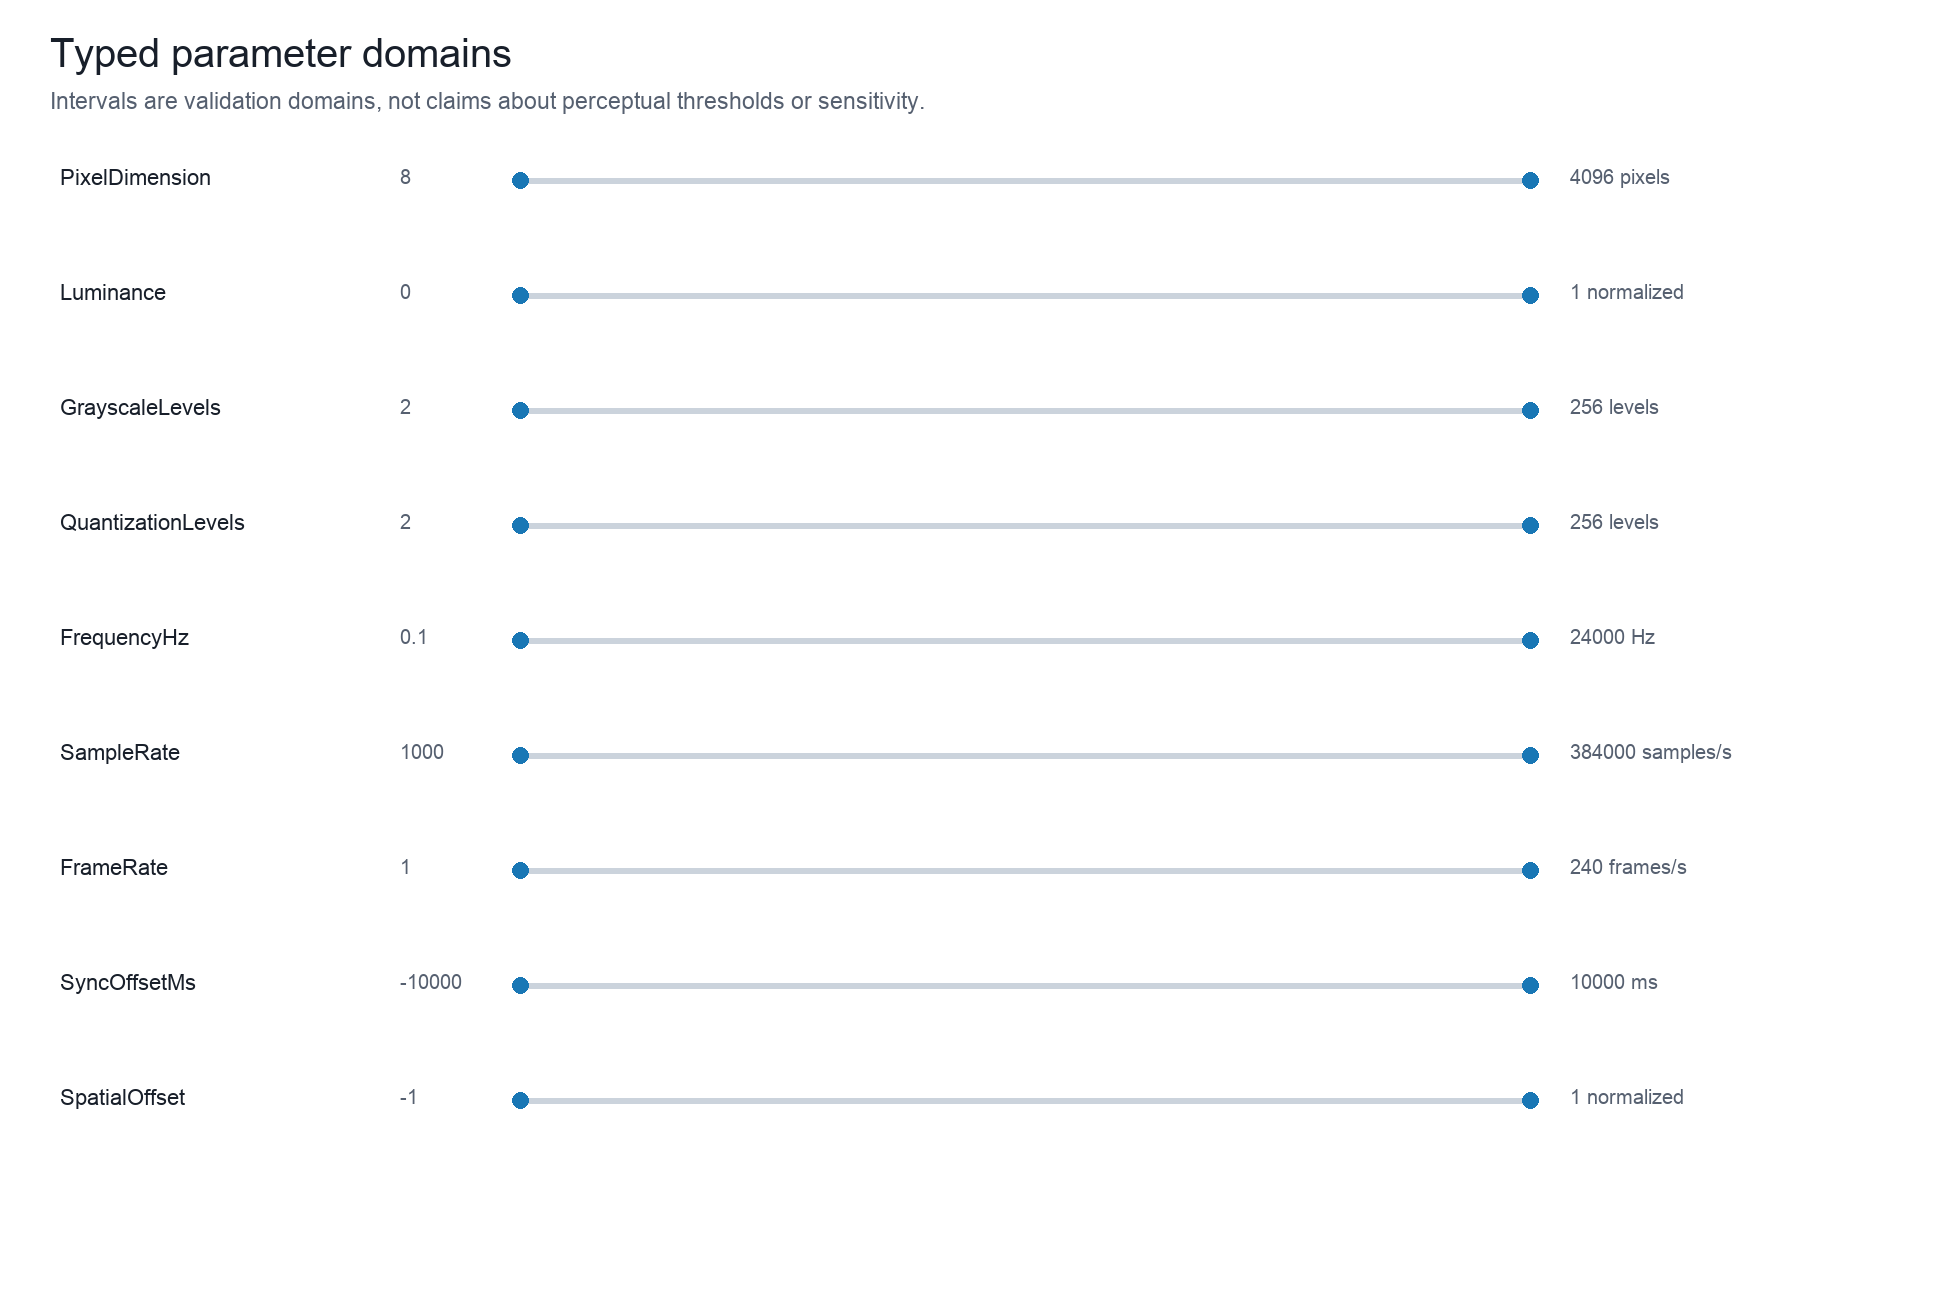
\includegraphics[keepaspectratio,alt={Horizontal interval markers show typed domains for dimensions, luminance, levels, frequency, sampling, frame rate, synchronization, and spatial discrepancy.}]{../figures/parameter_domains.png}}
\caption{Horizontal interval markers show typed domains for dimensions,
luminance, levels, frequency, sampling, frame rate, synchronization, and
spatial discrepancy.}\label{fig:parameter_domains}
\end{figure}

What this figure shows: Horizontal interval markers show typed domains
for dimensions, luminance, levels, frequency, sampling, frame rate,
synchronization, and spatial discrepancy. The domain map shows the
validated ranges for dimensions, luminance, grayscale and quantization
levels, frequency, sampling rate, frame rate, synchronization offset,
and spatial discrepancy. Source data output/data/parameter\_domains.json
records the type name, unit, interval, and engineering role; intervals
prevent malformed media and are not proposed as sensitivity thresholds.
Controls: parameter schema version and validated scalar domains; seed
not applicable to the domain diagram. Objective facts: dimensionless,
pixel, level, Hz, samples/s, frames/s, ms, and normalized spatial units
as listed per parameter. Claim level: canonical\_stimulus. Source data:
output/data/parameter\_domains.json (SHA-256 digest recorded in the
figure registry). Evidence lineage: formalism:eq:typed\_request.
Limitations: The intervals are software validation bounds and do not
encode safe listening levels, display limits, or psychophysical
thresholds. Boundary: A valid parameter is a reproducible construction
request, not evidence that the requested value is perceptually
effective.

The domain map fig.~\ref{fig:parameter_domains} is a validation
visualization. Bounds are chosen to prevent malformed media and unsafe
encodings, not to predict a viewer, listener, or participant's
sensitivity.

\subsection{Observer-design boundary}\label{observer-design-boundary}

\begin{figure}
\centering
\pandocbounded{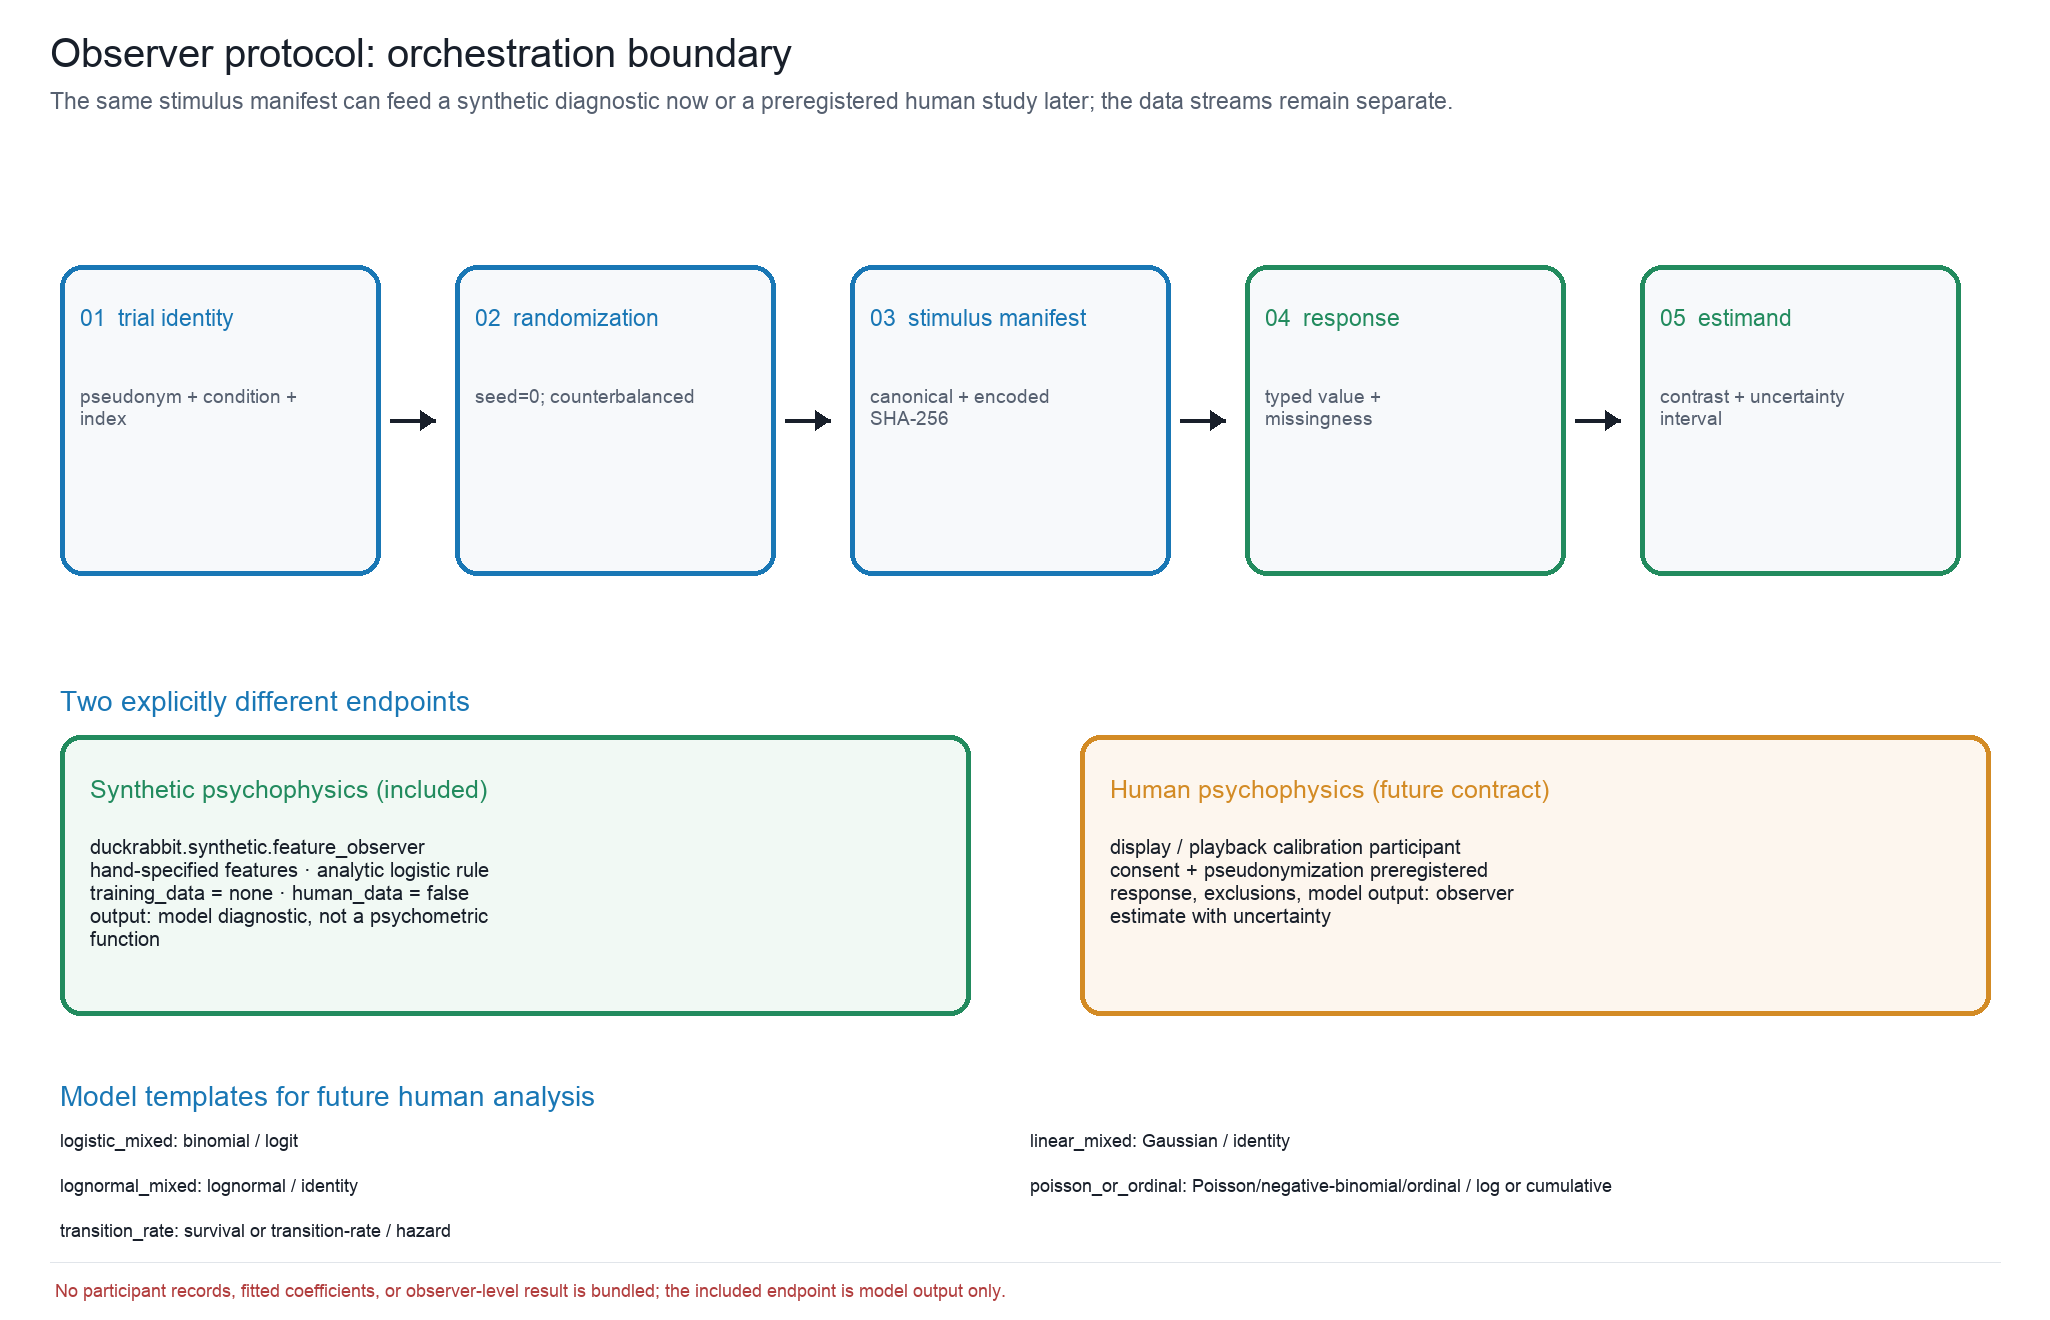
\includegraphics[keepaspectratio,alt={A flow diagram connects trial identity, randomization, stimulus manifest, response, aggregate estimand, and analysis-model templates, with a synthetic-only boundary.}]{../figures/observer_protocol.png}}
\caption{A flow diagram connects trial identity, randomization, stimulus
manifest, response, aggregate estimand, and analysis-model templates,
with a synthetic-only boundary.}\label{fig:observer_protocol}
\end{figure}

What this figure shows: A flow diagram connects trial identity,
randomization, stimulus manifest, response, aggregate estimand, and
analysis-model templates, with a synthetic-only boundary. The
study-ready scaffold moves from pseudonymous trial identity and
deterministic randomization to a stimulus manifest and encoded-file
hash, typed response or missingness, and a preregistered estimand.
Source data output/data/observer\_protocol.json records the study
design, randomization seed, model templates, and synthetic-only status;
no participant record is included. Controls: study design and
deterministic randomization seed recorded in the sidecar; synthetic
response generation is separate from human data. Objective facts: trial
counts, condition structure, estimand templates, response schemas, and
model families; participant outcomes are not applicable. Claim level:
observer\_hypothesis. Source data: output/data/observer\_protocol.json
(SHA-256 digest recorded in the figure registry). Evidence lineage:
observer:preregistered\_estimands. Limitations: The scaffold specifies
future data collection and analysis but supplies no participant
responses, fitted coefficients, power claim, or validated observer
effect. Boundary: The protocol is ready for ethical and preregistered
extension, not evidence that the proposed effect exists.

The observer scaffold fig.~\ref{fig:observer_protocol} starts with a
pseudonymous trial identity and deterministic randomization, binds the
stimulus manifest and encoded hash, records a typed response or
missingness state, and ends at a preregistered estimand. The companion
diagnostic fig.~\ref{fig:synthetic_psychophysics} is a deterministic,
hand-specified feature observer with \breaktt{training\_data=none} and
\breaktt{human\_data=false}; it is not a pretrained vision model,
psychometric function, or participant result. Human psychophysics
remains a future evidence layer requiring calibrated playback, consent,
preregistration, and observed responses.

\subsection{Generated audit tables}\label{generated-audit-tables}

\begin{longtable}[]{@{}
  >{\raggedright\arraybackslash}p{(\linewidth - 6\tabcolsep) * \real{0.2500}}
  >{\raggedright\arraybackslash}p{(\linewidth - 6\tabcolsep) * \real{0.2500}}
  >{\raggedright\arraybackslash}p{(\linewidth - 6\tabcolsep) * \real{0.2500}}
  >{\raggedright\arraybackslash}p{(\linewidth - 6\tabcolsep) * \real{0.2500}}@{}}
\caption{Code-owned caption, source-data, and accessibility
audit.}\label{tbl:caption_audit}\tabularnewline
\toprule\noalign{}
\begin{minipage}[b]{\linewidth}\raggedright
Figure / claim level
\end{minipage} & \begin{minipage}[b]{\linewidth}\raggedright
Source and evidence
\end{minipage} & \begin{minipage}[b]{\linewidth}\raggedright
Controls and objective facts
\end{minipage} & \begin{minipage}[b]{\linewidth}\raggedright
Limitations, boundary, and accessibility
\end{minipage} \\
\midrule\noalign{}
\endfirsthead
\toprule\noalign{}
\begin{minipage}[b]{\linewidth}\raggedright
Figure / claim level
\end{minipage} & \begin{minipage}[b]{\linewidth}\raggedright
Source and evidence
\end{minipage} & \begin{minipage}[b]{\linewidth}\raggedright
Controls and objective facts
\end{minipage} & \begin{minipage}[b]{\linewidth}\raggedright
Limitations, boundary, and accessibility
\end{minipage} \\
\midrule\noalign{}
\endhead
\bottomrule\noalign{}
\endlastfoot
fig:architecture; canonical stimulus & output/data/architecture.json;
formalism:eq:typed request, formalism:eq:canonical generation,
formalism:eq:encoding verification & Controls: typed request q=(i,\texorpdfstring{\ensuremath{\theta}}{theta},s,e)
with seed s=0; default generator and delivery-independent
canonicalization Objective: no unit-bearing objective quantity is
applicable to this architecture diagram; stage identities and provenance
fields are recorded in the sidecar & Limitations: The schematic
abstracts implementation boundaries and does not represent an observer
study or a causal theory of perception. Boundary: The pipeline verifies
reproducible media facts, not what a person experiences. Accessibility:
Stage names, mathematical symbols, and arrow direction are printed
directly; color is redundant. \\
fig:catalog matrix; source supported & output/data/catalog matrix.json;
gregory1997visual, hirst2020sound, bruns2019ventriloquist & Controls:
live taxonomy registry; evidence matrix snapshot; seed not applicable to
the catalog diagram Objective: 18 catalog rows; categorical facets and
statuses; no observer-level quantity is applicable & Limitations:
Taxonomy facets are engineering classifications and remain provisional
where the literature supports competing accounts. Boundary: Catalog
coverage is bounded to this registered package and does not enumerate
all known illusions. Accessibility: Every status and facet is written as
text; color only reinforces the printed status. \\
fig:visual panel; canonical stimulus & output/data/visual panel.json;
gregory1997visual, brugger1999duckrabbit, howe2005muller,
morgan1999poggendorff, fisher1967ponzo, yildiz2022ponzo,
kanizsa1976contours, mruczek2015ebbinghaus, earle1995zollner,
wertheimer1912motion, sekuler1996wertheimer & Controls: one default
typed parameter object per implemented visual entry; seed s=0;
dimensions, luminance bounds, grayscale, and quantization controls
remain in each generator schema; temporal entries display their first
frame but retain sequence metrics Objective: per tile: mean and
standard-deviation relative luminance, unique raster levels, and
canonical SHA-256 digest; temporal entries additionally retain frame
count, frame rate, and frame deltas; definitions and units are in the
source data JSON & Limitations: The gallery is complete for implemented
visual entries in this package, not a complete survey of visual
illusions; literature families, historical displays, and DuckRabbit
rasters are not pixel-identical by default. Viewing scale, display
calibration, viewing distance, and observer conditions can change the
relevance of a construction; the gallery does not measure an observer's
perceptual report. Boundary: The figure establishes coverage of the
package's implemented visual constructions and their deterministic
raster facts. It does not establish that any viewer will perceive the
named signature, nor that the set is exhaustive of the visual-illusion
literature. Accessibility: Each tile is labeled by stable illusion ID
and accompanied by printed luminance, level-count, and digest fields;
color only reinforces grouping and is not required to identify a
stimulus. \\
fig:visual sweep; physical metric & output/data/visual sweep.json;
brugger1999duckrabbit, gregory1997visual & Controls: duck weight \texorpdfstring{\ensuremath{\in}}{in}
\{0,.25,.5,.75,1\}; grayscale=quantization \texorpdfstring{\ensuremath{\in}}{in} \{2,4,8,16,32\}; seed s=0
Objective: 25 canonical rasters; unique levels, normalized mean
luminance, and effective dynamic range per cell & Limitations: The grid
is a sensitivity of the construction parameters, not a psychophysical
sensitivity curve or a validated observer effect. Boundary: The chosen
grid is an engineering sampling of the parameter domain and does not
imply an optimal or perceptually uniform spacing. Accessibility: Row and
column labels state the parameter values; numerical metrics and units
are available in the sidecar. \\
fig:temporal sequence; physical metric & output/data/temporal
sequence.json; wertheimer1912motion, sekuler1996wertheimer & Controls:
visual.apparent motion default typed parameters; frame rate and frame
count from the canonical sequence; seed s=0 Objective: timestamps in
seconds, frame rate in frames/s, frame count, rational timebase, and
adjacent-frame normalized pixel difference & Limitations: Frame
succession and frame deltas are physical file properties; playback
timing, display persistence, and motion reports require a controlled
observer task. Boundary: The figure documents temporal structure rather
than the presence, direction, or strength of perceived motion.
Accessibility: Frame index, seconds, frames per second, and
normalized-difference labels remain interpretable without color. \\
fig:audio signals; physical metric & output/data/audio signals.json;
shepard1984scale, zatorre2005missing, deutsch1986tritone,
repp1997tritone, deutsch1974octave, warren1970continuity,
riecke2011continuity & Controls: default typed audio parameters;
per-generator channel layout and sample rate; seed s=0; one-sided FFT
display with 48 sampled bins Objective: RMS and peak in normalized
amplitude; spectral centroid and bandwidth in Hz; sample rate in
samples/s; channel layout and canonical SHA-256 digest & Limitations:
Playback level, transducer response, dichotic separation, masker design,
and listener judgments are external to the canonical buffer. Boundary:
The figure compares generated signal properties and literature-linked
families; it does not establish pitch, continuity, or stream
organization for a listener. Accessibility: Waveform, spectral,
amplitude, and frequency labels are printed; bar color is not the sole
encoding. \\
fig:audiovisual timeline; physical metric & output/data/audiovisual
timeline.json; shams2000sifi, hirst2020sound, vroomen2004temporal,
hartcherobrien2011temporal & Controls: audiovisual.sound induced flash
default shared timeline; declared sync offset \texorpdfstring{\ensuremath{\Delta}}{Delta}AV and spatial offset;
seed s=0 Objective: video luminance and audio envelope on normalized
shared time; \texorpdfstring{\ensuremath{\Delta}}{Delta}AV in ms; spatial discrepancy in normalized units; frame
and sample clocks in the sidecar & Limitations: Display refresh, audio
hardware, event latency, and observer temporal binding are not measured
by this figure. Boundary: A shared-clock construction is not evidence
that observers bind the events at the declared or any other perceptual
time. Accessibility: The two channels, time axis, signed offset
convention, and normalized spatial discrepancy are labeled in text. \\
fig:encoding verification; encoded media & output/data/encoding
verification.json; engineering:typed media adapters & Controls: typed
encoding profile selected per artifact; overwrite and backend capability
checks; seed inherited from the stimulus request Objective: format
availability and verification scope are environment observations; NPZ is
exact while other formats are decoded and tolerance-checked &
Limitations: Backend availability, codec versions, container metadata,
and lossy tolerances are environment-dependent; playback software can
expose additional behavior. Boundary: A successful encode or decode does
not validate an observer effect or guarantee cross-device perceptual
equivalence. Accessibility: Format, backend, preserved fact, and
verification columns are textual and remain usable without color. \\
fig:synthetic psychophysics; synthetic model output &
output/data/synthetic psychophysics.json; observer:preregistered
estimands & Controls: duck weight comparison against fixed reference;
serialized feature weights and temperature; seed s=0 Objective: model
probability and score delta on the displayed model-output scale;
canonical stimulus digests; human data=false; training data=none &
Limitations: The model is hand-specified, has no training data, has not
been calibrated against observers, and does not estimate a human
threshold or effect size. Its probabilities are model outputs, not
participant responses or a psychometric function. Boundary: This
diagnostic tests deterministic orchestration and metamorphic
input-output behavior only; empirical psychophysics remains future work.
Accessibility: Model scale, reference line, model identity, and
\breaktt{human\ data=false} are printed; color is not needed to interpret
the curve. \\
fig:claim boundary; source supported & output/data/claim boundary.json;
formalism:eq:observer estimand, formalism:eq:canonical digest &
Controls: claim levels in the taxonomy and manifest; seed not applicable
to the explanatory diagram Objective: no unit-bearing objective quantity
is applicable; stage definitions and evidence boundaries are preserved
in the sidecar & Limitations: The diagram is a documentation contract
and does not replace a preregistered observer study or empirical data.
Boundary: A deterministic artifact can support a future hypothesis but
cannot supply the observer data required to test it. Accessibility: Each
stage is named, numbered, and described in text; the boundary rule is
readable without color. \\
fig:scholarship map; source supported & output/data/scholarship
map.json; gregory1997visual, brugger1999duckrabbit, yildiz2022ponzo,
hirst2020sound, bruns2019ventriloquist & Controls: checked-in evidence
matrix; source roles and entry statuses; audit date recorded in
data/evidence matrix.json Objective: one evidence row per catalog entry
(18 entries); source-tier counts, exact claim text, engineering basis,
limitation, and gap status & Limitations: The offline snapshot validates
citation and lineage structure; live resolver status is a separate
audit, and classifications can remain contested. Boundary: Scholarship
coverage bounds the package's evidence record and does not establish
that any generated stimulus produces a universal percept. Accessibility:
Source roles, claims, limitations, and statuses are printed or available
in the sidecar; no category is encoded by color alone. \\
fig:formalism traceability; physical metric & output/data/formalism
traceability.json; formalism:eq:canonical digest, formalism:eq:clock
definition, formalism:eq:objective statistics & Controls: formalism
registry version; seed not applicable to the traceability diagram
Objective: nine equation records with implementation, test, figure, and
claim-level fields; no unit-bearing measurement is plotted &
Limitations: Traceability records documentation and verification scope;
it does not establish the truth of an observer-level theory. Boundary: A
linked equation and test can show an implemented contract, not a
validated perceptual law. Accessibility: Equation labels, code paths,
tests, and figure labels are written as text. \\
fig:metrics dashboard; physical metric & output/data/metrics
dashboard.json; formalism:eq:objective statistics, formalism:eq:temporal
spectral metrics & Controls: default canonical artifacts; metric
computation version and tolerance recorded in the source-data sidecar;
seed s=0 Objective: finite objective values with units: normalized
luminance/amplitude, Hz, normalized pixel difference, ms, counts, and
durations & Limitations: Metrics are media properties and do not encode
pitch, size, motion, localization, binding, or other observer
interpretations. Boundary: Metric reproducibility is a package property;
interpretation as perception requires a separate observer design and
data. Accessibility: Every numerical value is paired with a printed unit
or an explicit dimensionless definition. \\
fig:parameter domains; canonical stimulus & output/data/parameter
domains.json; formalism:eq:typed request & Controls: parameter schema
version and validated scalar domains; seed not applicable to the domain
diagram Objective: dimensionless, pixel, level, Hz, samples/s, frames/s,
ms, and normalized spatial units as listed per parameter & Limitations:
The intervals are software validation bounds and do not encode safe
listening levels, display limits, or psychophysical thresholds.
Boundary: A valid parameter is a reproducible construction request, not
evidence that the requested value is perceptually effective.
Accessibility: Type names, endpoints, units, and roles are printed;
interval color is redundant. \\
fig:observer protocol; observer hypothesis & output/data/observer
protocol.json; observer:preregistered estimands & Controls: study design
and deterministic randomization seed recorded in the sidecar; synthetic
response generation is separate from human data Objective: trial counts,
condition structure, estimand templates, response schemas, and model
families; participant outcomes are not applicable & Limitations: The
scaffold specifies future data collection and analysis but supplies no
participant responses, fitted coefficients, power claim, or validated
observer effect. Boundary: The protocol is ready for ethical and
preregistered extension, not evidence that the proposed effect exists.
Accessibility: Every protocol step and the no-participant-data boundary
is stated in text; arrows and labels remain legible without color. \\
\end{longtable}

\begin{longtable}[]{@{}
  >{\raggedright\arraybackslash}p{(\linewidth - 8\tabcolsep) * \real{0.2000}}
  >{\raggedright\arraybackslash}p{(\linewidth - 8\tabcolsep) * \real{0.2000}}
  >{\raggedright\arraybackslash}p{(\linewidth - 8\tabcolsep) * \real{0.2000}}
  >{\raggedright\arraybackslash}p{(\linewidth - 8\tabcolsep) * \real{0.2000}}
  >{\raggedright\arraybackslash}p{(\linewidth - 8\tabcolsep) * \real{0.2000}}@{}}
\caption{Source-tiered evidence, DOI/URL verification, exact supported
claims, engineering departures, limitations, and explicit
planned/input-required gaps.}\label{tbl:evidence_audit}\tabularnewline
\toprule\noalign{}
\begin{minipage}[b]{\linewidth}\raggedright
Key
\end{minipage} & \begin{minipage}[b]{\linewidth}\raggedright
Record and citations
\end{minipage} & \begin{minipage}[b]{\linewidth}\raggedright
DOI and URL
\end{minipage} & \begin{minipage}[b]{\linewidth}\raggedright
Verification
\end{minipage} & \begin{minipage}[b]{\linewidth}\raggedright
Supported claim / engineering / limitation
\end{minipage} \\
\midrule\noalign{}
\endfirsthead
\toprule\noalign{}
\begin{minipage}[b]{\linewidth}\raggedright
Key
\end{minipage} & \begin{minipage}[b]{\linewidth}\raggedright
Record and citations
\end{minipage} & \begin{minipage}[b]{\linewidth}\raggedright
DOI and URL
\end{minipage} & \begin{minipage}[b]{\linewidth}\raggedright
Verification
\end{minipage} & \begin{minipage}[b]{\linewidth}\raggedright
Supported claim / engineering / limitation
\end{minipage} \\
\midrule\noalign{}
\endhead
\bottomrule\noalign{}
\endlastfoot
gregory 1997 visual & review; gregory 1997 visual & DOI: recorded; URL
host/path: pubmed.ncbi.nlm.nih.gov & snapshot validated; offline
snapshot & A non-exhaustive classification of visual illusion
families. \\
hirst 2020 sound & review; hirst 2020 sound & DOI: recorded; URL
host/path: www.sciencedirect.com & snapshot validated; offline snapshot
& A review of sound-induced flash paradigms and multisensory temporal
inference. \\
howe 2005 muller & theory; howe 2005 muller & DOI: recorded; URL
host/path: doi.org & snapshot validated; offline snapshot & A
statistical image-source account of Müller-Lyer geometry. \\
morgan 1999 poggendorff & theory; morgan 1999 poggendorff & DOI:
recorded; URL host/path: doi.org & snapshot validated; offline snapshot
& A mechanistic account of Poggendorff orientation estimation. \\
fisher 1967 ponzo & primary; fisher 1967 ponzo & DOI: recorded; URL
host/path: www.nature.com & snapshot validated; offline snapshot & A
primary investigation of identical targets embedded in an angular
context. \\
kanizsa 1976 contours & primary; kanizsa 1976 contours & DOI: recorded;
URL host/path: pubmed.ncbi.nlm.nih.gov & snapshot validated; offline
snapshot & Canonical illusory-contour inducer arrangements. \\
mruczek 2015 ebbinghaus & primary; mruczek 2015 ebbinghaus & DOI:
recorded; URL host/path: pmc.ncbi.nlm.nih.gov & snapshot validated;
offline snapshot & Context-dependent size judgments in Ebbinghaus-family
stimuli. \\
wertheimer 1912 motion & primary; wertheimer 1912 motion & DOI: not
recorded; URL host/path: bibbase.org & snapshot validated; offline
snapshot & Foundational apparent-motion experiments using successive
spatial events. \\
sekuler 1996 wertheimer & review; sekuler 1996 wertheimer & DOI:
recorded; URL host/path: journals.sagepub.com & snapshot validated;
offline snapshot & A review connecting Wertheimer's successive-event
findings to later apparent-motion research and clarifying their
historical scope. \\
shepard 1984 scale & primary; shepard 1984 scale & DOI: recorded; URL
host/path: doi.org & snapshot validated; offline snapshot & Auditory
scale and pitch-class organization in Shepard-like tones. \\
zatorre 2005 missing & review; zatorre 2005 missing & DOI: recorded; URL
host/path: doi.org & snapshot validated; offline snapshot & The
missing-fundamental problem as a pitch-inference phenomenon. \\
deutsch 1986 tritone & primary; deutsch 1986 tritone & DOI: recorded;
URL host/path: online.ucpress.edu & snapshot validated; offline snapshot
& The tritone paradox and dependence on pitch-class context and
listener. \\
deutsch 1974 octave & primary; deutsch 1974 octave & DOI: recorded; URL
host/path: doi.org & snapshot validated; offline snapshot & Dichotic
alternating high/low tone construction underlying the octave
illusion. \\
shams 2000 sifi & primary; shams 2000 sifi & DOI: recorded; URL
host/path: doi.org & snapshot validated; offline snapshot & The
one-flash/two-beep sound-induced flash contrast. \\
bruns 2019 ventriloquist & review; bruns 2019 ventriloquist & DOI:
recorded; URL host/path: pmc.ncbi.nlm.nih.gov & snapshot validated;
offline snapshot & Spatial audiovisual capture and multisensory
integration constraints. \\
vroomen 2004 temporal & primary; vroomen 2004 temporal & DOI: recorded;
URL host/path: pubmed.ncbi.nlm.nih.gov & snapshot validated; offline
snapshot & Sound timing can alter the apparent temporal structure of a
visual event. \\
mcgurk 1976 speech & primary; mcgurk 1976 speech & DOI: recorded; URL
host/path: doi.org & snapshot validated; offline snapshot &
Speech-dependent audiovisual categorical integration, requiring
validated fixtures. \\
warren 1970 continuity & primary; warren 1970 continuity & DOI:
recorded; URL host/path: doi.org & snapshot validated; offline snapshot
& Auditory continuity/restoration as a future calibrated masker
family. \\
brugger 1999 duckrabbit & primary; brugger 1999 duckrabbit & DOI:
recorded; URL host/path: pubmed.ncbi.nlm.nih.gov & snapshot validated;
offline snapshot & Variation in duck/rabbit ambiguity across figure
variants and observers. \\
yildiz 2022 ponzo & review; yildiz 2022 ponzo & DOI: recorded; URL
host/path: pubmed.ncbi.nlm.nih.gov & snapshot validated; offline
snapshot & Competing depth-based and non-depth-based explanations of
Ponzo-like illusions. \\
repp 1997 tritone & primary; repp 1997 tritone & DOI: recorded; URL
host/path: pubmed.ncbi.nlm.nih.gov & snapshot validated; offline
snapshot & Listener- and context-dependent effects of spectral envelope
and pitch-class structure in tritone judgments. \\
hartcherobrien 2011 temporal & primary; hartcherobrien 2011 temporal &
DOI: recorded; URL host/path: pubmed.ncbi.nlm.nih.gov & snapshot
validated; offline snapshot & Audiovisual timing can shift temporal
judgments in a purely temporal context without spatial grounding. \\
earle 1995 zollner & primary; earle 1995 zollner & DOI: recorded; URL
host/path: journals.sagepub.com & snapshot validated; offline snapshot &
Crossing oblique and long-line geometry used to measure orientation
interactions in the Zöllner family. \\
zoellner 1860 pseudoscopy & primary; zoellner 1860 pseudoscopy & DOI:
recorded; URL host/path: onlinelibrary.wiley.com & snapshot validated;
offline snapshot & The nineteenth-century primary description of the
crossing-line orientation family later known as the Zöllner illusion. \\
riecke 2011 continuity & primary; riecke 2011 continuity & DOI:
recorded; URL host/path: doi.org & snapshot validated; offline snapshot
& Interrupted sounds with masking context and the separation of sensory
and decisional contributions. \\
wagemans 2012 gestalt & review; wagemans 2012 gestalt & DOI: recorded;
URL host/path: pubmed.ncbi.nlm.nih.gov & snapshot validated; offline
snapshot & Contemporary perceptual-grouping, contour-completion, and
figure-ground accounts relevant to Kanizsa-type constructions. \\
weintraub 1979 ebbinghaus & primary; weintraub 1979 ebbinghaus & DOI:
recorded; URL host/path: pubmed.ncbi.nlm.nih.gov & snapshot validated;
offline snapshot & A classic contextual-size experiment varying surround
geometry and comparison conditions in Ebbinghaus-family displays. \\
noppeney 2018 causal & review; noppeney 2018 causal & DOI: recorded; URL
host/path: doi.org & snapshot validated; offline snapshot &
Causal-inference and temporal-prediction accounts of audiovisual
integration and segregation. \\
alhazen 1989 optics & primary; alhazen 1989 optics & DOI: not recorded;
URL host/path: www.cca.qc.ca & snapshot validated; offline snapshot &
The English translation and commentary preserves Ibn al-Haytham's
eleventh-century Arabic optics as a historical source on direct vision
and geometrical image formation. \\
mozi 2023 canons & review; mozi 2023 canons & DOI: recorded; URL
host/path: link.springer.com & snapshot validated; offline snapshot & A
modern translation and commentary documents Mohist Canon sections on
knowledge, optics, and mechanics, providing a Chinese Warring
States-period context for early technical reasoning about vision. \\
ptolemy 1996 optics & primary; ptolemy 1996 optics & DOI: not recorded;
URL host/path: sites.dlib.nyu.edu & snapshot validated; offline snapshot
& The scholarly translation makes Ptolemy's second-century Optics
available as an early work on visual perception and mathematical visual
theory. \\
berkeley 1709 vision & primary; berkeley 1709 vision & DOI: not
recorded; URL host/path: www.maths.tcd.ie & snapshot validated; offline
snapshot & Berkeley's 1709 essay treats visual distance and space as
mediated by learned associations rather than as a simple direct readout
of visual geometry. \\
kircher 1646 light & primary; kircher 1646 light & DOI: not recorded;
URL host/path: collections.st-andrews.ac.uk & snapshot validated;
offline snapshot & The digitized record anchors Kircher's 1646 Ars magna
lucis et umbrae as an early-modern work on light, shadow, and optical
display. \\
molyneux 2020 problem & review; molyneux 2020 problem & DOI: not
recorded; URL host/path: plato.stanford.edu & snapshot validated;
offline snapshot & The historical account documents Molyneux's 1688
question separating tactile learning from visual recognition and its
long cross-sensory afterlife. \\
cheselden 1728 sight & primary; cheselden 1728 sight & DOI: not
recorded; URL host/path: archive.org & snapshot validated; offline
snapshot & The digitized Philosophical Transactions record preserves
Cheselden's 1728 case report as a historical observation relevant to
visual access and the separation of observer evidence from stimulus
description. \\
dai 2015 chinesescience & review; dai 2015 chinesescience & DOI:
recorded; URL host/path: link.springer.com & snapshot validated; offline
snapshot & A history of Chinese science and technology surveys ancient
Chinese physics and records optical phenomena as part of a non-European
history of visual science. \\
entry / visual.duck rabbit & engineering / limitation / gap; brugger
1999 duckrabbit; gregory 1997 visual & DOI: n/a; URL host/path:
data/evidence\_matrix.json & snapshot validated; offline snapshot & The
entry instantiates a controllable ambiguous-figure stimulus family.
Engineering basis: Parameterized ambiguous silhouette; not a
pixel-identical reproduction of a historical plate. Limitation: The
generator verifies geometry and luminance, not bistable reports. Missing
contract: none \\
entry / visual.simultaneous contrast & engineering / limitation / gap;
gregory 1997 visual & DOI: n/a; URL host/path:
data/evidence\_matrix.json & snapshot validated; offline snapshot & The
physical center patches are matched while surround luminance differs.
Engineering basis: Equal central patches on unequal luminance surrounds.
Limitation: Display calibration and observer adaptation are not modeled.
Missing contract: none \\
entry / visual.apparent motion & engineering / limitation / gap;
wertheimer 1912 motion; sekuler 1996 wertheimer & DOI: n/a; URL
host/path: data/evidence\_matrix.json & snapshot validated; offline
snapshot & The sequence contains controlled successive spatial events.
Engineering basis: Alternating rectangular masks at a fixed rational
frame rate. Limitation: The artifact establishes temporal succession,
not perceived motion. Missing contract: none \\
entry / audio.shepard tone & engineering / limitation / gap; shepard
1984 scale & DOI: n/a; URL host/path: data/evidence\_matrix.json &
snapshot validated; offline snapshot & The audio contains octave-related
partials with controlled sweep parameters. Engineering basis: Additive
octave-spaced partials with a deterministic envelope. Limitation:
Playback transducers and listener pitch judgments are external. Missing
contract: none \\
entry / audio.missing fundamental & engineering / limitation / gap;
zatorre 2005 missing & DOI: n/a; URL host/path:
data/evidence\_matrix.json & snapshot validated; offline snapshot & The
nominal fundamental component is absent from the canonical spectrum.
Engineering basis: Harmonic components are synthesized while the nominal
fundamental is omitted. Limitation: Pitch completion is an
observer-level inference. Missing contract: none \\
entry / audiovisual.sound induced flash & engineering / limitation /
gap; shams 2000 sifi; hirst 2020 sound & DOI: n/a; URL host/path:
data/evidence\_matrix.json & snapshot validated; offline snapshot & The
declared beep/flash event counts and offsets are physically encoded.
Engineering basis: One flash paired with one or two timed beeps on a
shared clock. Limitation: The stimulus does not establish a reported
flash count. Missing contract: none \\
entry / audiovisual.ventriloquist & engineering / limitation / gap;
bruns 2019 ventriloquist; noppeney 2018 causal & DOI: n/a; URL
host/path: data/evidence\_matrix.json & snapshot validated; offline
snapshot & The audio and visual channels carry a declared spatial
discrepancy. Engineering basis: Stereo panning and visual displacement
encode a spatial discrepancy. Limitation: Perceived localization depends
on room, headphones, display, and observer. Missing contract: none \\
entry / visual.muller lyer & engineering / limitation / gap; gregory
1997 visual; howe 2005 muller & DOI: n/a; URL host/path:
data/evidence\_matrix.json & snapshot validated; offline snapshot & The
two bar lengths are equal in the canonical raster while wing geometry
varies. Engineering basis: Equal bars with controlled arrow-wing
geometry. Limitation: The chosen normalized geometry is one engineering
variant. Missing contract: none \\
entry / visual.poggendorff & engineering / limitation / gap; gregory
1997 visual; morgan 1999 poggendorff & DOI: n/a; URL host/path:
data/evidence\_matrix.json & snapshot validated; offline snapshot & The
occluder and diagonal continuation are generated from explicit geometry.
Engineering basis: A diagonal continuation is separated by a rectangular
occluder. Limitation: Alignment judgments and orientation filters are
not measured. Missing contract: none \\
entry / visual.ponzo & engineering / limitation / gap; fisher 1967
ponzo; yildiz 2022 ponzo & DOI: n/a; URL host/path:
data/evidence\_matrix.json & snapshot validated; offline snapshot &
Target bars are physically equal and rails converge toward a vanishing
region. Engineering basis: Equal target bars are placed inside
converging rails. Limitation: Perspective interpretation is observer-
and display-dependent. Missing contract: none \\
entry / visual.kanizsa triangle & engineering / limitation / gap;
kanizsa 1976 contours; wagemans 2012 gestalt & DOI: n/a; URL host/path:
data/evidence\_matrix.json & snapshot validated; offline snapshot & The
image contains incomplete inducers with no explicitly drawn triangle
edge. Engineering basis: Three incomplete circular inducers are
rasterized around a triangular gap. Limitation: Illusory contour
completion is not directly measured. Missing contract: none \\
entry / visual.ebbinghaus & engineering / limitation / gap; mruczek 2015
ebbinghaus; weintraub 1979 ebbinghaus & DOI: n/a; URL host/path:
data/evidence\_matrix.json & snapshot validated; offline snapshot &
Central target geometry is held equal while contextual circle geometry
differs. Engineering basis: Equal central targets are surrounded by
different context-circle sizes. Limitation: Perceived size depends on
viewing scale and context. Missing contract: none \\
entry / visual.zollner & engineering / limitation / gap; zoellner 1860
pseudoscopy; earle 1995 zollner; gregory 1997 visual & DOI: n/a; URL
host/path: data/evidence\_matrix.json & snapshot validated; offline
snapshot & The entry instantiates a controlled crossing-line orientation
stimulus family. Engineering basis: Vertical long lines crossed by short
oblique inducers with explicit normalized spacing and angle. Limitation:
The raster verifies line geometry, not orientation judgments or a
pixel-identical historical reproduction. Missing contract: none \\
entry / audio.tritone paradox & engineering / limitation / gap; deutsch
1986 tritone; repp 1997 tritone & DOI: n/a; URL host/path:
data/evidence\_matrix.json & snapshot validated; offline snapshot & The
canonical pair has an explicit half-octave frequency relation.
Engineering basis: Two octave-complex tones are separated by a
half-octave interval. Limitation: Ascending/descending reports vary
across listeners and contexts. Missing contract: none \\
entry / audio.octave illusion & engineering / limitation / gap; deutsch
1974 octave & DOI: n/a; URL host/path: data/evidence\_matrix.json &
snapshot validated; offline snapshot & The two channels receive
alternating octave-related tones. Engineering basis: Alternating high
and low tones are assigned to opposite stereo channels. Limitation: The
auditory percept depends on dichotic presentation and listener. Missing
contract: none \\
entry / audio.auditory continuity & engineering / limitation / gap;
warren 1970 continuity; riecke 2011 continuity & DOI: n/a; URL
host/path: data/evidence\_matrix.json & snapshot validated; offline
snapshot & The canonical audio contains a reproducible interruption
interval and masker family. Engineering basis: An interrupted sinusoidal
carrier is replaced during a declared gap by a deterministic tone or
white-noise masker with typed amplitude. Limitation: The generator
reports the physical interruption and masker, not a listener's
continuity judgment or sensory-versus-decisional effect. Missing
contract: none \\
entry / audiovisual.temporal ventriloquism & engineering / limitation /
gap; vroomen 2004 temporal; hartcherobrien 2011 temporal; hirst 2020
sound; noppeney 2018 causal & DOI: n/a; URL host/path:
data/evidence\_matrix.json & snapshot validated; offline snapshot &
Audio and video event timing and declared offset are deterministic and
inspectable. Engineering basis: A visual flash and audio click share a
clock with explicit offset. Limitation: The generated single-event pair
is a simplified engineering stimulus. Missing contract: none \\
entry / audiovisual.mcgurk & engineering / limitation / gap; mcgurk 1976
speech & DOI: n/a; URL host/path: data/evidence\_matrix.json & snapshot
validated; offline snapshot & The catalog identifies a speech-dependent
audiovisual family without claiming implementation. Engineering basis:
Requires validated speech audio/video fixtures and licensing records.
Limitation: No fixture, consent record, or perceptual validation
contract is bundled. Missing contract: A licensed or consented
checksummed speech audio/video fixture, synchronization contract, and
preregistered perceptual validation protocol are required. \\
\end{longtable}

\begin{longtable}[]{@{}
  >{\raggedright\arraybackslash}p{(\linewidth - 6\tabcolsep) * \real{0.2500}}
  >{\raggedright\arraybackslash}p{(\linewidth - 6\tabcolsep) * \real{0.2500}}
  >{\raggedright\arraybackslash}p{(\linewidth - 6\tabcolsep) * \real{0.2500}}
  >{\raggedright\arraybackslash}p{(\linewidth - 6\tabcolsep) * \real{0.2500}}@{}}
\caption{Formal equation-to-code
traceability.}\label{tbl:formalism}\tabularnewline
\toprule\noalign{}
\begin{minipage}[b]{\linewidth}\raggedright
Label
\end{minipage} & \begin{minipage}[b]{\linewidth}\raggedright
Definition and symbols
\end{minipage} & \begin{minipage}[b]{\linewidth}\raggedright
Implementation and tests
\end{minipage} & \begin{minipage}[b]{\linewidth}\raggedright
Figures and claim level
\end{minipage} \\
\midrule\noalign{}
\endfirsthead
\toprule\noalign{}
\begin{minipage}[b]{\linewidth}\raggedright
Label
\end{minipage} & \begin{minipage}[b]{\linewidth}\raggedright
Definition and symbols
\end{minipage} & \begin{minipage}[b]{\linewidth}\raggedright
Implementation and tests
\end{minipage} & \begin{minipage}[b]{\linewidth}\raggedright
Figures and claim level
\end{minipage} \\
\midrule\noalign{}
\endhead
\bottomrule\noalign{}
\endlastfoot
eq:typed request & q = (i, \texorpdfstring{\ensuremath{\theta}}{theta}, s, e) Symbols: i, \texorpdfstring{\ensuremath{\theta}}{theta}, s, e & Code:
registry.py, schema.py; Tests: test generators.py & Figures:
fig:architecture, fig:formalism traceability; Level: canonical
stimulus \\
eq:canonical generation & A = G\texorpdfstring{\textsubscript{i}}{i}(\texorpdfstring{\ensuremath{\theta}}{theta}; s) Symbols: A, G\texorpdfstring{\textsubscript{i}}{i}, \texorpdfstring{\ensuremath{\theta}}{theta}, s & Code:
registry.py, generators.py; Tests: test generators.py, test v03
contracts.py & Figures: fig:architecture, fig:visual panel; Level:
canonical stimulus \\
eq:canonical digest & c(A) = Serialize\_LE,float32(A, shape, clock,
units); h\_c(A) = H(c(A)) Symbols: c(A), h\_c, H & Code: canonical.py,
manifest.py; Tests: test v03 contracts.py & Figures: fig:architecture,
fig:encoding verification; Level: physical metric \\
eq:encoding verification & F = E\texorpdfstring{\textsubscript{e}}{e}(A), I = D(F), V(F, M) \texorpdfstring{\ensuremath{\in}}{in} \{pass, fail\}
Symbols: F, E\texorpdfstring{\textsubscript{e}}{e}, D, I, V, M & Code: render.py, inspection.py,
manifest.py; Tests: test media and render.py, test v03 contracts.py &
Figures: fig:encoding verification; Level: encoded media \\
eq:clock definition & N = round(f\_s T), t\_k = k/f\_r, \texorpdfstring{\ensuremath{\Delta}}{Delta}\_AV = t\_audio
\texorpdfstring{\ensuremath{-}}{-} t\_video Symbols: N, f\_s, T, t\_k, f\_r, \texorpdfstring{\ensuremath{\Delta}}{Delta}\_AV & Code: parameters.py,
artifacts.py; Tests: test parameters.py, test media and render.py &
Figures: fig:temporal sequence, fig:audiovisual timeline; Level:
physical metric \\
eq:objective statistics & \texorpdfstring{\ensuremath{\mu}}{mu}\_Y, \texorpdfstring{\ensuremath{\sigma}}{sigma}\_Y, RMS\_X = M(A; units, tolerance,
version) Symbols: \texorpdfstring{\ensuremath{\mu}}{mu}\_Y, \texorpdfstring{\ensuremath{\sigma}}{sigma}\_Y, RMS\_X, M & Code: metrics.py,
publication.py; Tests: test v04 scholarly.py & Figures: fig:metrics
dashboard, fig:audio signals; Level: physical metric \\
eq:temporal spectral metrics & D\_k = mean absolute difference of
adjacent frames; centroid(X) = \texorpdfstring{\ensuremath{\Sigma}}{Sigma} fP\_X(f)/\texorpdfstring{\ensuremath{\Sigma}}{Sigma}P\_X(f) Symbols: D\_k, P\_X,
f & Code: metrics.py, artifacts.py; Tests: test v04 scholarly.py &
Figures: fig:temporal sequence, fig:metrics dashboard; Level: physical
metric \\
eq:observer estimand & \texorpdfstring{\ensuremath{\psi}}{psi} = E{[}Y conditional on condition and
protocol{]} Symbols: \texorpdfstring{\ensuremath{\psi}}{psi}, Y, condition, protocol & Code: observer
analysis.py, observer.py; Tests: test v04 scholarly.py & Figures:
fig:synthetic psychophysics, fig:observer protocol; Level: observer
hypothesis \\
eq:synthetic observer & p\_M(c given A\_r,A\_c) = \texorpdfstring{\ensuremath{\sigma}}{sigma}((w\texorpdfstring{\ensuremath{\cdot}}{.}\texorpdfstring{\ensuremath{\varphi}}{phi}(A\_c) \texorpdfstring{\ensuremath{-}}{-}
w\texorpdfstring{\ensuremath{\cdot}}{.}\texorpdfstring{\ensuremath{\varphi}}{phi}(A\_r))/\texorpdfstring{\ensuremath{\tau}}{tau}) Symbols: p\_M, c, A\_r, A\_c, w, \texorpdfstring{\ensuremath{\varphi}}{phi}, \texorpdfstring{\ensuremath{\tau}}{tau} & Code: synthetic
psychophysics.py, metrics.py; Tests: test synthetic psychophysics.py &
Figures: fig:synthetic psychophysics; Level: synthetic model output \\
\end{longtable}

\begin{longtable}[]{@{}
  >{\raggedright\arraybackslash}p{(\linewidth - 6\tabcolsep) * \real{0.2500}}
  >{\raggedright\arraybackslash}p{(\linewidth - 6\tabcolsep) * \real{0.2500}}
  >{\raggedright\arraybackslash}p{(\linewidth - 6\tabcolsep) * \real{0.2500}}
  >{\raggedright\arraybackslash}p{(\linewidth - 6\tabcolsep) * \real{0.2500}}@{}}
\caption{Claim ledger separating code-derived facts, scholarship,
engineering departures, limitations, scope, and observer
hypotheses.}\label{tbl:claim_ledger}\tabularnewline
\toprule\noalign{}
\begin{minipage}[b]{\linewidth}\raggedright
Claim ID
\end{minipage} & \begin{minipage}[b]{\linewidth}\raggedright
Claim and level
\end{minipage} & \begin{minipage}[b]{\linewidth}\raggedright
Basis
\end{minipage} & \begin{minipage}[b]{\linewidth}\raggedright
Lineage and limitation
\end{minipage} \\
\midrule\noalign{}
\endfirsthead
\toprule\noalign{}
\begin{minipage}[b]{\linewidth}\raggedright
Claim ID
\end{minipage} & \begin{minipage}[b]{\linewidth}\raggedright
Claim and level
\end{minipage} & \begin{minipage}[b]{\linewidth}\raggedright
Basis
\end{minipage} & \begin{minipage}[b]{\linewidth}\raggedright
Lineage and limitation
\end{minipage} \\
\midrule\noalign{}
\endhead
\bottomrule\noalign{}
\endlastfoot
catalog:count & The catalog contains 18 entries. Level:
canonical\_stimulus & derived\_from\_code & Lineage: taxonomy entries()
Limitation: Catalog membership is not a completeness claim about all
known illusions. Manuscript: manuscript/09 appendix catalog.md \\
evidence:source count & The checked-in evidence matrix contains 36
source records. Level: source\_supported & checked\_in\_scholarship &
Lineage: data/evidence matrix.json::sources Limitation: The offline
snapshot does not imply that every URL is currently reachable or that a
source supports more than its exact record. Manuscript: manuscript/06
scope and related work.md \\
scope:no participant data & No participant data are bundled with the
package. Level: observer\_hypothesis & derived\_from\_code & Lineage:
experiments/observer protocol.md; output/data/synthetic
psychophysics.json Limitation: Future observer studies require
preregistration, consent, calibrated presentation, and separate data
governance. Manuscript: manuscript/07 publication audit.md \\
synthetic:diagnostic boundary & The synthetic observer is a
deterministic model-output diagnostic, not human psychophysics. Level:
synthetic\_model\_output & synthetic\_model\_output & Lineage:
src/duckrabbit/synthetic psychophysics.py; output/data/synthetic
psychophysics.json Limitation: The hand-specified model has no training
data and has not been calibrated against observers. Manuscript:
manuscript/02 methodology.md \\
cover:editorial boundary & The cover is a publication illustration, not
an experimental stimulus or observer result. Level:
publication\_illustration & publication\_illustration & Lineage:
output/reports/cover visualization.json Limitation: The editorial asset
is not part of the deterministic scientific stimulus registry.
Manuscript: manuscript/07 publication audit.md \\
evidence:visual.duck rabbit & The entry instantiates a controllable
ambiguous-figure stimulus family. Level: source\_supported &
checked\_in\_scholarship & Lineage: sources=brugger1999duckrabbit;
gregory1997visual; data/evidence matrix.json; engineering=Parameterized
ambiguous silhouette; not a pixel-identical reproduction of a historical
plate.; limitation=The generator verifies geometry and luminance, not
bistable reports.; missing contract=none Limitation: The generator
verifies geometry and luminance, not bistable reports. Manuscript:
manuscript/06 scope and related work.md \\
evidence:visual.simultaneous contrast & The physical center patches are
matched while surround luminance differs. Level: source\_supported &
checked\_in\_scholarship & Lineage: sources=gregory1997visual;
data/evidence matrix.json; engineering=Equal central patches on unequal
luminance surrounds.; limitation=Display calibration and observer
adaptation are not modeled.; missing contract=none Limitation: Display
calibration and observer adaptation are not modeled. Manuscript:
manuscript/06 scope and related work.md \\
evidence:visual.apparent motion & The sequence contains controlled
successive spatial events. Level: source\_supported &
checked\_in\_scholarship & Lineage: sources=wertheimer1912motion;
sekuler1996wertheimer; data/evidence matrix.json;
engineering=Alternating rectangular masks at a fixed rational frame
rate.; limitation=The artifact establishes temporal succession, not
perceived motion.; missing contract=none Limitation: The artifact
establishes temporal succession, not perceived motion. Manuscript:
manuscript/06 scope and related work.md \\
evidence:audio.shepard tone & The audio contains octave-related partials
with controlled sweep parameters. Level: source\_supported &
checked\_in\_scholarship & Lineage: sources=shepard1984scale;
data/evidence matrix.json; engineering=Additive octave-spaced partials
with a deterministic envelope.; limitation=Playback transducers and
listener pitch judgments are external.; missing contract=none
Limitation: Playback transducers and listener pitch judgments are
external. Manuscript: manuscript/06 scope and related work.md \\
evidence:audio.missing fundamental & The nominal fundamental component
is absent from the canonical spectrum. Level: source\_supported &
checked\_in\_scholarship & Lineage: sources=zatorre2005missing;
data/evidence matrix.json; engineering=Harmonic components are
synthesized while the nominal fundamental is omitted.; limitation=Pitch
completion is an observer-level inference.; missing contract=none
Limitation: Pitch completion is an observer-level inference. Manuscript:
manuscript/06 scope and related work.md \\
evidence:audiovisual.sound induced flash & The declared beep/flash event
counts and offsets are physically encoded. Level: source\_supported &
checked\_in\_scholarship & Lineage: sources=shams2000sifi;
hirst2020sound; data/evidence matrix.json; engineering=One flash paired
with one or two timed beeps on a shared clock.; limitation=The stimulus
does not establish a reported flash count.; missing contract=none
Limitation: The stimulus does not establish a reported flash count.
Manuscript: manuscript/06 scope and related work.md \\
evidence:audiovisual.ventriloquist & The audio and visual channels carry
a declared spatial discrepancy. Level: source\_supported &
checked\_in\_scholarship & Lineage: sources=bruns2019ventriloquist;
noppeney2018causal; data/evidence matrix.json; engineering=Stereo
panning and visual displacement encode a spatial discrepancy.;
limitation=Perceived localization depends on room, headphones, display,
and observer.; missing contract=none Limitation: Perceived localization
depends on room, headphones, display, and observer. Manuscript:
manuscript/06 scope and related work.md \\
evidence:visual.muller lyer & The two bar lengths are equal in the
canonical raster while wing geometry varies. Level: source\_supported &
checked\_in\_scholarship & Lineage: sources=gregory1997visual;
howe2005muller; data/evidence matrix.json; engineering=Equal bars with
controlled arrow-wing geometry.; limitation=The chosen normalized
geometry is one engineering variant.; missing contract=none Limitation:
The chosen normalized geometry is one engineering variant. Manuscript:
manuscript/06 scope and related work.md \\
evidence:visual.poggendorff & The occluder and diagonal continuation are
generated from explicit geometry. Level: source\_supported &
checked\_in\_scholarship & Lineage: sources=gregory1997visual;
morgan1999poggendorff; data/evidence matrix.json; engineering=A diagonal
continuation is separated by a rectangular occluder.;
limitation=Alignment judgments and orientation filters are not
measured.; missing contract=none Limitation: Alignment judgments and
orientation filters are not measured. Manuscript: manuscript/06 scope
and related work.md \\
evidence:visual.ponzo & Target bars are physically equal and rails
converge toward a vanishing region. Level: source\_supported &
checked\_in\_scholarship & Lineage: sources=fisher1967ponzo;
yildiz2022ponzo; data/evidence matrix.json; engineering=Equal target
bars are placed inside converging rails.; limitation=Perspective
interpretation is observer- and display-dependent.; missing
contract=none Limitation: Perspective interpretation is observer- and
display-dependent. Manuscript: manuscript/06 scope and related
work.md \\
evidence:visual.kanizsa triangle & The image contains incomplete
inducers with no explicitly drawn triangle edge. Level:
source\_supported & checked\_in\_scholarship & Lineage:
sources=kanizsa1976contours; wagemans2012gestalt; data/evidence
matrix.json; engineering=Three incomplete circular inducers are
rasterized around a triangular gap.; limitation=Illusory contour
completion is not directly measured.; missing contract=none Limitation:
Illusory contour completion is not directly measured. Manuscript:
manuscript/06 scope and related work.md \\
evidence:visual.ebbinghaus & Central target geometry is held equal while
contextual circle geometry differs. Level: source\_supported &
checked\_in\_scholarship & Lineage: sources=mruczek2015ebbinghaus;
weintraub1979ebbinghaus; data/evidence matrix.json; engineering=Equal
central targets are surrounded by different context-circle sizes.;
limitation=Perceived size depends on viewing scale and context.; missing
contract=none Limitation: Perceived size depends on viewing scale and
context. Manuscript: manuscript/06 scope and related work.md \\
evidence:visual.zollner & The entry instantiates a controlled
crossing-line orientation stimulus family. Level: source\_supported &
checked\_in\_scholarship & Lineage: sources=zoellner1860pseudoscopy;
earle1995zollner; gregory1997visual; data/evidence matrix.json;
engineering=Vertical long lines crossed by short oblique inducers with
explicit normalized spacing and angle.; limitation=The raster verifies
line geometry, not orientation judgments or a pixel-identical historical
reproduction.; missing contract=none Limitation: The raster verifies
line geometry, not orientation judgments or a pixel-identical historical
reproduction. Manuscript: manuscript/06 scope and related work.md \\
evidence:audio.tritone paradox & The canonical pair has an explicit
half-octave frequency relation. Level: source\_supported &
checked\_in\_scholarship & Lineage: sources=deutsch1986tritone;
repp1997tritone; data/evidence matrix.json; engineering=Two
octave-complex tones are separated by a half-octave interval.;
limitation=Ascending/descending reports vary across listeners and
contexts.; missing contract=none Limitation: Ascending/descending
reports vary across listeners and contexts. Manuscript: manuscript/06
scope and related work.md \\
evidence:audio.octave illusion & The two channels receive alternating
octave-related tones. Level: source\_supported &
checked\_in\_scholarship & Lineage: sources=deutsch1974octave;
data/evidence matrix.json; engineering=Alternating high and low tones
are assigned to opposite stereo channels.; limitation=The auditory
percept depends on dichotic presentation and listener.; missing
contract=none Limitation: The auditory percept depends on dichotic
presentation and listener. Manuscript: manuscript/06 scope and related
work.md \\
evidence:audio.auditory continuity & The canonical audio contains a
reproducible interruption interval and masker family. Level:
source\_supported & checked\_in\_scholarship & Lineage:
sources=warren1970continuity; riecke2011continuity; data/evidence
matrix.json; engineering=An interrupted sinusoidal carrier is replaced
during a declared gap by a deterministic tone or white-noise masker with
typed amplitude.; limitation=The generator reports the physical
interruption and masker, not a listener's continuity judgment or
sensory-versus-decisional effect.; missing contract=none Limitation: The
generator reports the physical interruption and masker, not a listener's
continuity judgment or sensory-versus-decisional effect. Manuscript:
manuscript/06 scope and related work.md \\
evidence:audiovisual.temporal ventriloquism & Audio and video event
timing and declared offset are deterministic and inspectable. Level:
source\_supported & checked\_in\_scholarship & Lineage:
sources=vroomen2004temporal; hartcherobrien2011temporal; hirst2020sound;
noppeney2018causal; data/evidence matrix.json; engineering=A visual
flash and audio click share a clock with explicit offset.;
limitation=The generated single-event pair is a simplified engineering
stimulus.; missing contract=none Limitation: The generated single-event
pair is a simplified engineering stimulus. Manuscript: manuscript/06
scope and related work.md \\
evidence:audiovisual.mcgurk & The catalog identifies a speech-dependent
audiovisual family without claiming implementation. Level:
source\_supported & checked\_in\_scholarship & Lineage:
sources=mcgurk1976speech; data/evidence matrix.json;
engineering=Requires validated speech audio/video fixtures and licensing
records.; limitation=No fixture, consent record, or perceptual
validation contract is bundled.; missing contract=A licensed or
consented checksummed speech audio/video fixture, synchronization
contract, and preregistered perceptual validation protocol are required.
Limitation: No fixture, consent record, or perceptual validation
contract is bundled. Manuscript: manuscript/06 scope and related
work.md \\
publication:figure count & The publication atlas contains 15 registered
scientific figures. Level: physical\_metric & derived\_from\_code &
Lineage: publication caption specs() Limitation: The count is a
package-state fact, not evidence of empirical validity. Manuscript:
manuscript/07 publication audit.md \\
publication:table count & The publication appendix contains the
generated table set defined by the publication table payload registry.
Level: physical\_metric & derived\_from\_code & Lineage: publication
table payloads() Limitation: Generated tables summarize package state
and do not replace source or observer evidence. Manuscript:
manuscript/07 publication audit.md \\
\end{longtable}

The source-tiered evidence table tbl.~\ref{tbl:evidence_audit}, caption
audit tbl.~\ref{tbl:caption_audit}, formalism registry
tbl.~\ref{tbl:formalism}, and claim ledger tbl.~\ref{tbl:claim_ledger}
are generated sidecars. They provide a publication appendix without
duplicating mutable counts or silently converting literature statements
into package results.

The publication artifacts have two distinct provenance boundaries.
Scientific figures are deterministic PNG renders whose source-data JSON
and SHA-256 digests are checked against the code-owned registry. The
cover is an editorial charcoal illustration: its selected candidate,
prompt fingerprint, source asset digest, dimensions, variants, and
provenance boundary are recorded in
\breaktt{output/reports/cover\_visualization.json}. Neither boundary is
an observer result, and neither substitutes for display calibration or
behavioral data.

The publication audit additionally resolves every formalism edge to a
real package module, test file, manuscript equation label, and
registered figure. Figure source-data sidecars use a versioned schema
with figure identity, generator, seed, and nested data payload; the
registry verifies this identity and hash independently of the renderer.
This makes a visually plausible but stale or relabeled figure fail the
same provenance gate as a tampered stimulus.

\newpage

\section{Discussion and Conclusion}\label{sec:discussion}

DuckRabbit's principal result is a reproducibility boundary rather than
a new psychophysical finding. The same typed request can be regenerated,
hashed, encoded, decoded, and audited, while the evidence graph and
observer layer remain explicit about what the package cannot infer. This
makes the atlas useful for stimulus construction, source comparison, and
preregistration without treating a rendered image or sound as behavioral
evidence.

The scholarly contribution is correspondingly modest but operational.
Rather than flattening visual, auditory, temporal, and multisensory
families into a single ``illusion'' label, the package keeps mechanism,
perceptual signature, requirements, evidence role, engineering basis,
and implementation status separate. A primary demonstration, a review, a
theoretical account, and a source describing the DuckRabbit
implementation answer different questions. The appendix and source-data
sidecars make those distinctions inspectable at the same time as the
generated media.

The work is best understood as a research-software artifact with a
bounded methods contribution. Its novelty claim is not that it discovers
a new illusion or resolves a disputed mechanism; it is that a
heterogeneous stimulus catalog can be represented as typed,
reproducible, source-linked, and release-audited objects. This framing
is consistent with software-citation and FAIR guidance, which treats
versioned software, metadata, provenance, and reuse conditions as part
of the research record
\citep{smith2016software, wilkinson2016fair, lamprecht2020fairsoftware}.

The release is authored by Daniel Ari Friedman of the Active Inference
Institute and is published and citable at
\href{https://github.com/docxology/DuckRabbit}{the DuckRabbit public
GitHub repository}. The generated bundle in this repository remains the
authoritative release candidate until the external template handoff is
completed.

\subsection{Conclusion}\label{sec:conclusion}

DuckRabbit v0.5.0 turns multimodal illusion generation into an auditable
typed pipeline. A request produces a canonical artifact, objective
metrics, optional delivery files, decoded inspection, and a versioned
evidence-bounded manifest. The catalog now records not only what is
implemented, but also what the literature supports and what remains
unvalidated.

The main scientific contribution is a boundary: deterministic stimulus
facts are reproducible software outputs, while perceptual effects are
hypotheses that require observer conditions and data. This boundary
permits broad generator coverage without overclaiming. Future additions
should contribute a typed parameter contract, a literature record, an
engineering-fidelity statement, objective invariants, generated
documentation, and tests before entering the implemented registry.
Promotion is a release decision about software readiness, not a verdict
on whether a perceptual phenomenon is real.

The synthetic-psychophysics layer extends this boundary without crossing
it. A transparent feature observer makes model inputs, weights,
calibration, and output hashes inspectable, so the full orchestration
can be tested today. Its small curve is a diagnostic of that specified
model, not evidence that humans share its feature map or response
function. Empirical observer work remains a separate, ethically and
methodologically governed stage.

\newpage

\section{Appendix A. Complete catalog, source tiers, and
evidence/implementation boundaries}\label{sec:appendix_catalog}

This appendix is the authoritative rendered snapshot of DuckRabbit's
live catalog. It is generated from the taxonomy registry and evidence
matrix during the publication build; the table is not hand-maintained.
The snapshot records the package's current scope, not a claim to
enumerate every illusion described in the literature.

\subsection{How to read the matrix}\label{how-to-read-the-matrix}

Each row identifies a registered illusion family and separates five
questions that are often collapsed in informal catalogs:

\begin{enumerate}
\def\labelenumi{\arabic{enumi}.}
\tightlist
\item
  What modality, mechanism, and signature does the package assign to the
  construction?
\item
  What evidence and implementation status does the checked-in record
  support?
\item
  Which sources support the exact statement written in the row?
\item
  What physical claim is supported by the row?
\item
  What full source role, resolver, DOI status, and claim level are
  retained in the machine-readable record?
\end{enumerate}

\texttt{implemented} means that DuckRabbit has a deterministic generator
and a validated canonical artifact contract. It does not mean that the
generated stimulus is a pixel-identical reproduction of a historical
experiment or that an observer effect has been re-established.
\texttt{input\_required} means that the family remains catalogued but
lacks a lawful, checksummed input fixture and/or the validation contract
required for deterministic generation. Evidence status and
implementation status are deliberately independent.

The source column is a compact citation-key view. The full source role,
resolver or DOI status, exact supported claim, engineering departure,
and limitation are retained in the machine-readable evidence matrix and
in the generated evidence audit tbl.~\ref{tbl:evidence_audit}. A source
supports only the narrow claim recorded for it; a review or theory
record is not evidence that a DuckRabbit rendering produces a universal
perceptual effect.

\begin{longtable}[]{@{}
  >{\raggedright\arraybackslash}p{(\linewidth - 8\tabcolsep) * \real{0.2000}}
  >{\raggedright\arraybackslash}p{(\linewidth - 8\tabcolsep) * \real{0.2000}}
  >{\raggedright\arraybackslash}p{(\linewidth - 8\tabcolsep) * \real{0.2000}}
  >{\raggedright\arraybackslash}p{(\linewidth - 8\tabcolsep) * \real{0.2000}}
  >{\raggedright\arraybackslash}p{(\linewidth - 8\tabcolsep) * \real{0.2000}}@{}}
\caption{DuckRabbit catalog entries, source tiers, and
evidence/implementation boundaries.}\label{tbl:catalog}\tabularnewline
\toprule\noalign{}
\begin{minipage}[b]{\linewidth}\raggedright
ID
\end{minipage} & \begin{minipage}[b]{\linewidth}\raggedright
Construction
\end{minipage} & \begin{minipage}[b]{\linewidth}\raggedright
Evidence / status
\end{minipage} & \begin{minipage}[b]{\linewidth}\raggedright
Sources
\end{minipage} & \begin{minipage}[b]{\linewidth}\raggedright
Supported claim
\end{minipage} \\
\midrule\noalign{}
\endfirsthead
\toprule\noalign{}
\begin{minipage}[b]{\linewidth}\raggedright
ID
\end{minipage} & \begin{minipage}[b]{\linewidth}\raggedright
Construction
\end{minipage} & \begin{minipage}[b]{\linewidth}\raggedright
Evidence / status
\end{minipage} & \begin{minipage}[b]{\linewidth}\raggedright
Sources
\end{minipage} & \begin{minipage}[b]{\linewidth}\raggedright
Supported claim
\end{minipage} \\
\midrule\noalign{}
\endhead
\bottomrule\noalign{}
\endlastfoot
visual.duck rabbit & visual; ambiguity; bistability & literature backed
engineering entry; implemented & brugger 1999 duckrabbit; gregory 1997
visual & The entry instantiates a controllable ambiguous-figure stimulus
family. \\
visual.simultaneous contrast & visual; contrast and context; contrast
distortion & literature backed engineering entry; implemented & gregory
1997 visual & The physical center patches are matched while surround
luminance differs. \\
visual.apparent motion & visual; temporal motion; illusory motion &
literature backed engineering entry; implemented & wertheimer 1912
motion; sekuler 1996 wertheimer & The sequence contains controlled
successive spatial events. \\
audio.shepard tone & auditory; spectral harmonic; continuity &
literature backed engineering entry; implemented & shepard 1984 scale &
The audio contains octave-related partials with controlled sweep
parameters. \\
audio.missing fundamental & auditory; spectral harmonic; filling in &
literature backed engineering entry; implemented & zatorre 2005 missing
& The nominal fundamental component is absent from the canonical
spectrum. \\
audiovisual.sound induced flash & audio\_visual; crossmodal temporal;
fusion or fission & review backed engineering entry; implemented & shams
2000 sifi; hirst 2020 sound & The declared beep/flash event counts and
offsets are physically encoded. \\
audiovisual.ventriloquist & audio\_visual; crossmodal spatial; spatial
capture & review backed engineering entry; implemented & bruns 2019
ventriloquist; noppeney 2018 causal & The audio and visual channels
carry a declared spatial discrepancy. \\
visual.muller lyer & visual; geometric alignment; geometric distortion &
literature backed engineering entry; implemented & gregory 1997 visual;
howe 2005 muller & The two bar lengths are equal in the canonical raster
while wing geometry varies. \\
visual.poggendorff & visual; geometric alignment; geometric distortion &
literature backed engineering entry; implemented & gregory 1997 visual;
morgan 1999 poggendorff & The occluder and diagonal continuation are
generated from explicit geometry. \\
visual.ponzo & visual; geometric alignment; geometric distortion &
literature backed engineering entry; implemented & fisher 1967 ponzo;
yildiz 2022 ponzo & Target bars are physically equal and rails converge
toward a vanishing region. \\
visual.kanizsa triangle & visual; contrast and context, geometric
alignment; filling in & literature backed engineering entry; implemented
& kanizsa 1976 contours; wagemans 2012 gestalt & The image contains
incomplete inducers with no explicitly drawn triangle edge. \\
visual.ebbinghaus & visual; contrast and context, geometric alignment;
geometric distortion & literature backed engineering entry; implemented
& mruczek 2015 ebbinghaus; weintraub 1979 ebbinghaus & Central target
geometry is held equal while contextual circle geometry differs. \\
visual.zollner & visual; geometric alignment; geometric distortion &
literature backed engineering entry; implemented & zoellner 1860
pseudoscopy; earle 1995 zollner; gregory 1997 visual & The entry
instantiates a controlled crossing-line orientation stimulus family. \\
audio.tritone paradox & auditory; spectral harmonic; categorical
recoding & literature backed engineering entry; implemented & deutsch
1986 tritone; repp 1997 tritone & The canonical pair has an explicit
half-octave frequency relation. \\
audio.octave illusion & auditory; stream segregation; fusion or fission
& literature backed engineering entry; implemented & deutsch 1974 octave
& The two channels receive alternating octave-related tones. \\
audio.auditory continuity & auditory; stream segregation; continuity &
literature backed engineering entry; implemented & warren 1970
continuity; riecke 2011 continuity & The canonical audio contains a
reproducible interruption interval and masker family. \\
audiovisual.temporal ventriloquism & audio\_visual; crossmodal temporal;
temporal binding or recalibration & review backed engineering entry;
implemented & vroomen 2004 temporal; hartcherobrien 2011 temporal; hirst
2020 sound; noppeney 2018 causal & Audio and video event timing and
declared offset are deterministic and inspectable. \\
audiovisual.mcgurk & audio\_visual; speech categorization; categorical
recoding & literature backed input dependent entry; input required &
mcgurk 1976 speech & The catalog identifies a speech-dependent
audiovisual family without claiming implementation. \\
\end{longtable}

\subsection{Evidence boundary and future
expansion}\label{evidence-boundary-and-future-expansion}

The matrix is intentionally a living registry snapshot. New families may
be added when the package can state a typed parameter contract,
deterministic canonicalization rule, validation invariant, and evidence
boundary. Planned or input-dependent families are not silently promoted
because a source exists: promotion requires an implementable contract,
reproducible fixtures where needed, and an explicit statement of what
remains unvalidated. McGurk therefore remains \texttt{input\_required}
pending a consented or licensed, checksummed speech/ video fixture and a
study-ready validation protocol. The candidate-future catalog is
documented separately from this live matrix so that absence is not
misread as a claim that a phenomenon is unknown or unimportant.

\newpage



\clearpage

\bibliography{references}
\end{document}
